% Compilation instructions: 
% ------------------------------------------------------------------
% Use pdflatex to compile! Input images are expected as PDF files.
% Example compilation:
% ------------------------------------------------------------------
% > pdflatex thesis-example.tex
% > bibtex thesis-example
% > pdflatex thesis-example.tex
% > pdflatex thesis-example.tex
% ------------------------------------------------------------------
% You need to run pdflatex multiple times so that all the cross-references
% are fixed. pdflatex will tell you if you need to re-run it (a warning
% will be issued)  
% ------------------------------------------------------------------
% Compilation has been tested to work in ukk.cs.hut.fi and kosh.hut.fi
% - if you have problems of missing .sty -files, then the local LaTeX
% environment does not have all the required packages installed.
% For example, when compiling in vipunen.hut.fi, you get an error that
% tikz.sty is missing - in this case you must either compile somewhere
% else, or you cannot use TikZ graphics in your thesis and must therefore
% remove or comment out the tikz package and all the tikz definitions. 
% ------------------------------------------------------------------

\documentclass[12pt,a4paper,oneside,pdftex]{report}
% The input files (tex files) are encoded with the latin-1 encoding 
% (ISO-8859-1 works). Change the latin1-option if you use UTF8 
% (at some point LaTeX did not work with UTF8, but I'm not sure
% what the current situation is) 
%\usepackage[latin1]{inputenc}
\usepackage[utf8]{inputenc}
% OT1 font encoding seems to work better than T1. Check the rendered
% PDF file to see if the fonts are encoded properly as vectors (instead
% of rendered bitmaps). You can do this by zooming very close to any letter 
% - if the letter is shown pixelated, you should change this setting 
% (try commenting out the entire line, for example).  
\usepackage[OT1]{fontenc}
\usepackage[english]{babel}

% Natbib allows you to select the format of the bibliography references.
% The first example uses numbered citations: 
\usepackage[square,sort&compress,numbers]{natbib}
% The second example uses author-year citations.
% If you use author-year citations, change the bibliography style (below); 
% acm style does not work with author-year citations.
% Also, you should use \citet (cite in text) when you wish to refer
% to the author directly (\citet{blaablaa} said blaa blaa), and 
% \citep when you wish to refer similarly than with numbered citations
% (It has been said that blaa blaa~\citep{blaablaa}).
% \usepackage[square]{natbib}


\usepackage{eurosym} 
\usepackage{longtable}
\usepackage{multirow} % multi row in tables
%\usepackage{pifont} % ding symbols
%\usepackage{pdfpages} % import pdf pages
\usepackage{subfigure}
%\usepackage{systeme}
\usepackage{verbatim}

% The TikZ package allows you to create professional technical figures.
% The learning curve is quite steep, but it is definitely worth it if 
% you wish to have really good-looking technical figures. 
\usepackage{tikz}
% You also need to specify which TikZ libraries you use
\usetikzlibrary{positioning}
\usetikzlibrary{calc}
\usetikzlibrary{arrows}
\usetikzlibrary{decorations.pathmorphing,decorations.markings}
\usetikzlibrary{shapes}
\usetikzlibrary{patterns}

\usepackage[mydraft,twosupervisors,doublenumbering]{aalto-thesis}

% Hyperref
% ------------------------------------------------------------------
% Hyperref creates links from URLs, for references, and creates a
% TOC in the PDF file.
% This package must be the last one you include, because it has
% compatibility issues with many other packages and it fixes
% those issues when it is loaded.   
%\RequirePackage[pdftex]{hyperref}
\RequirePackage[pdfa]{hyperref}
% Setup hyperref so that links are clickable but do not look 
% different
\hypersetup{colorlinks=false,raiselinks=false,breaklinks=true}
\hypersetup{pdfborder={0 0 0}}
\hypersetup{bookmarksnumbered=true}
% The following line suggests the PDF reader that it should show the 
% first level of bookmarks opened in the hierarchical bookmark view. 
\hypersetup{bookmarksopen=true,bookmarksopenlevel=1}
% Hyperref can also set up the PDF metadata fields. These are
% set a bit later on, after the thesis setup.   

% Thesis setup
% ==================================================================
% Change these to fit your own thesis.
% \COMMAND always refers to the English version;
% \FCOMMAND refers to the Finnish version; and
% \SCOMMAND refers to the Swedish version.
% You may comment/remove those language variants that you do not use
% (but then you must not include the abstracts for that language)
% ------------------------------------------------------------------
% If you do not find the command for a text that is shown in the cover page or
% in the abstract texts, check the aalto-thesis.sty file and locate the text
% from there. 
% All the texts are configured in language-specific blocks (lots of commands
% that look like this: \renewcommand{\ATCITY}{Espoo}.
% You can just fix the texts there. Just remember to check all the language
% variants you use (they are all there in the same place). 
% ------------------------------------------------------------------
\newcommand{\TITLE}{Structured light assisted real time stereo photogrammetry for robotics and automation} 
\newcommand{\SUBTITLE}{Novel implementation of stereo matching}
\newcommand{\DATE}{\date}

% Supervisors and instructors
% ------------------------------------------------------------------
% Usually thesis have one supervisor and one advisor. Sometimes you
% may have two advisors and, in double degree
% programs, you may have two supervisors. 
% If you have two supervisors, write both names here, separate them with a 
% double-backslash (see below for an example)
% Also remember to add the package option ``twosupervisors'' or
% ``twoinstructors'' to the aalto-thesis package (aalto-thesis.sty
% file line 72), so that the titles are in plural.

% Example of twosupervisors:
\newcommand{\SUPERVISOR}{Professor Juho Kannala\\
  Professor Nicola Conci}

% If you have only one instructor, just write one name here
\newcommand{\INSTRUCTOR}{Sami Ruuskanen M.Sc. (Tech.)}

% If you have two supervisors, it is common to write the schools
% of the supervisors in the cover page. If the following command is defined,
% then the supervisor names shown here are printed in the cover page. Otherwise,
% the supervisor names defined above are used.
\newcommand{\COVERSUPERVISOR}{Professor Juho Kannala, Aalto University\\
  Professor Nicola Conci, University of Trento}

% The same option is for the instructors, if you have multiple instructors.
% \newcommand{\COVERINSTRUCTOR}{Oili Ohjaaja M.Sc. (Tech.), Aalto University\\
%  Elli Opas M.Sc. (Tech), Aalto SCI}


% Other stuff
% ------------------------------------------------------------------
\newcommand{\PROFESSORSHIP}{Autonomous Systems}
% Professorship code is the same in all languages
\newcommand{\PROFCODE}{}
\newcommand{\KEYWORDS}{stereo vision; matching cost; census transform; hamming distance; binary pattern; semi-global matching}
\newcommand{\LANGUAGE}{English}

% Author is the same for all languages
\newcommand{\AUTHOR}{Jacopo Losi}


% Currently the English versions are used for the PDF file metadata
% Set the PDF title
\hypersetup{pdftitle={\TITLE\ \SUBTITLE}}
% Set the PDF author
\hypersetup{pdfauthor={\AUTHOR}}
% Set the PDF keywords
\hypersetup{pdfkeywords={\KEYWORDS}}
% Set the PDF subject
\hypersetup{pdfsubject={Master's Thesis}}


% Layout settings
% ------------------------------------------------------------------

% When you write in English, you should use the standard LaTeX 
% paragraph formatting: paragraphs are indented, and there is no 
% space between paragraphs.

% If you write your thesis Finnish, uncomment these lines; if 
% you write in English, leave these lines commented! 
% \setlength{\parindent}{0pt}
% \setlength{\parskip}{1ex}

% Use this to control how much space there is between each line of text.
% 1 is normal (no extra space), 1.3 is about one-half more space, and
% 1.6 is about double line spacing.  
% \linespread{1} % This is the default
% \linespread{1.3}

% Bibliography style
% acm style gives you a basic reference style. It works only with numbered
% references.
\bibliographystyle{ieeetr}
% Plainnat is a plain style that works with both numbered and name citations.
% \bibliographystyle{plainnat}


% Extra hyphenation settings
% ------------------------------------------------------------------
% You can list here all the files that are not hyphenated correctly.
% You can provide many \hyphenation commands and/or separate each word
% with a space inside a single command. Put hyphens in the places where
% a word can be hyphenated.
% Note that (by default) LaTeX will not hyphenate words that already
% have a hyphen in them (for example, if you write ``structure-modification 
% operation'', the word structure-modification will never be hyphenated).
% You need a special package to hyphenate those words.
% \hyphenation{di-gi-taa-li-sta yksi-suun-tai-sta}



% The preamble ends here, and the document begins. 
% Place all formatting commands and such before this line.
% ------------------------------------------------------------------
\begin{document}
% This command adds a PDF bookmark to the cover page. You may leave
% it out if you don't like it...
\pdfbookmark[0]{Cover page}{bookmark.0.cover}
% This command is defined in aalto-thesis.sty. It controls the page 
% numbering based on whether the doublenumbering option is specified
\startcoverpage

% Cover page
% ------------------------------------------------------------------
% Options: finnish, english, and swedish
% These control in which language the cover-page information is shown
\coverpage{english}


% Abstracts
% ------------------------------------------------------------------
% Include an abstract in the language that the thesis is written in,
% and if your native language is Finnish or Swedish, one in that language.

% Abstract in English
% ------------------------------------------------------------------
\thesisabstract{english}{
The abstract provides goal, motivation, background, and conclusions of
the work. It has to fit to one page together with the bibliographical
information. 

If the thesis is in English and the language of school
education is Finnish or Swedish, the abstract is written in English
and in Finnish or in Swedish. If the language of school education is
other than Finnish or Swedish, the abstract is written in English only.

The thesis example file (\texttt{thesis-example.tex}), all the chapter content
files (\texttt{1introduction.tex} and so on), and the Aalto style file
(\texttt{aalto-thesis.sty}) are commented with explanations on how the Aalto
thesis works. The files also contain some examples on how to customize various
details of the thesis layout, and of course the example text works as an
example in itself. Please read the comments and the example text; that should
get you well on your way!

In the thesis template, you can find the text of the abstract in the
abstract in the \texttt{thesis-example.tex}
file, together with the bibliographical information of the abstract tables.
\fixme{This is an example how to use fixme: add your abstract here.} 
Fixme is a command that helps you identify parts of your thesis that still
require some work. When compiled in the custom \texttt{mydraft} mode, text
parts tagged with fixmes are shown in bold and with fixme tags around them. When
compiled in normal mode, the fixme-tagged text is shown normally (without
special formatting). The draft mode also causes the ``Draft'' text to appear on
the front page, alongside with the document compilation date. The custom
\texttt{mydraft} mode is selected by the \texttt{mydraft} option given for the
package \texttt{aalto-thesis}, near the top of the \texttt{thesis-example.tex}
file.
}



% Acknowledgements
% ------------------------------------------------------------------
% Select the language you use in your acknowledgements
\selectlanguage{english}

% Uncomment this line if you wish acknoledgements to appear in the 
% table of contents
%\addcontentsline{toc}{chapter}{Acknowledgements}

% The star means that the chapter isn't numbered and does not 
% show up in the TOC
\chapter*{Acknowledgements}

I wish to thank all students who use \LaTeX\ for formatting their theses,
because theses formatted with \LaTeX\ are just so nice.

Thank you, and keep up the good work!
\vskip 10mm

\noindent Espoo, \DATE
\vskip 5mm
\noindent\AUTHOR

% Acronyms
% ------------------------------------------------------------------
% Use \cleardoublepage so that IF two-sided printing is used 
% (which is not often for masters theses), then the pages will still
% start correctly on the right-hand side.
\cleardoublepage
% Example acronyms are placed in a separate file, acronyms.tex
\addcontentsline{toc}{chapter}{Abbreviations and Acronyms}
\chapter*{Abbreviations and Acronyms}

% The longtable environment should break the table properly to multiple pages, 
% if needed

\noindent
\begin{longtable}{@{}p{0.25\textwidth}p{0.7\textwidth}@{}}
SGM & Semi-Global Matching. Stereo matching algorithm developed by Heiko Hirschm\"{u}ller \\
SGBM & Semi-Global Box Matching. Area-based version of the previous algorithm. The main changing stands in the aggregation cost phase that here is performed over a certain subregion for every pixel and not over the entire image dimensions.\\
MRF & Markov Random Field. Set of random variables having Markov property, described by undirected graph. \\ 
CNN & Convolutional Neural Network \\
MI & Mutual Information \\
DP & Dynamic Programming \\
PKR & Peak Ratio \\
LiDAR & Light detection and ranging \\
\end{longtable}


% Table of contents
% ------------------------------------------------------------------
\cleardoublepage
% This command adds a PDF bookmark that links to the contents.
% You can use \addcontentsline{} as well, but that also adds contents
% entry to the table of contents, which is kind of redundant.
% The text ``Contents'' is shown in the PDF bookmark. 
\pdfbookmark[0]{Contents}{bookmark.0.contents}
\tableofcontents

% List of tables
% ------------------------------------------------------------------
% You only need a list of tables for your thesis if you have very 
% many tables. If you do, uncomment the following two lines.
% \cleardoublepage
% \listoftables

% Table of figures
% ------------------------------------------------------------------
% You only need a list of figures for your thesis if you have very 
% many figures. If you do, uncomment the following two lines.
% \cleardoublepage
% \listoffigures

% The following label is used for counting the prelude pages
\label{pages-prelude}
\cleardoublepage

%%%%%%%%%%%%%%%%% The main content starts here %%%%%%%%%%%%%%%%%%%%%
% ------------------------------------------------------------------
% This command is defined in aalto-thesis.sty. It controls the page 
% numbering based on whether the doublenumbering option is specified
\startfirstchapter

% Add headings to pages (the chapter title is shown)
\pagestyle{headings}

% The contents of the thesis are separated to their own files.
% Edit the content in these files, rename them as necessary.
% ------------------------------------------------------------------
\chapter{Introduction}
\label{chapter:intro}

%Introduction tells the motivation, scope, goal and the outcome of the
%work. Anyone should be able to understand it. The preferred order of
%writing your master's thesis is about the same as the outline of the
%thesis: you first discover your problem and write about that, then you
%find out what methods you should use and write about that.  Then you
%do your implementation, and document that, and so on.  However, the
%abstract and introduction are often easiest to write last.  This is
%because these really cover the entire thesis, and there is no way you
%could know what to put in your abstract before you have actually done
%your implementation and evaluation. This means that you have to
%rewrite them in the end of your work.

%By the way, rarely anyone write the thesis from the beginning to the
%end just one time, but the writing is more like process, where every
%piece of text is written at least twice. Be also prepared to delete
%your own text. In the first phase, you can hide it into comments that
%are started with \% but during the writing, the many comments should
%be visible for your helpers, the advisor(s) and supervisor.

%Read the information from the university master's thesis
%pages~\cite{ThesisInstructions} before starting the thesis.  You
%should also go through the thesis grading
%instructions~\cite{ThesisGrading} together with your advisor and/or
%supervisor in the beginning of your work.

%The introduction in itself is rarely very long; two to five pages
%often suffice. It usually has two subsections with titles Problem
%statement and Structure of the Thesis, as follows next.


\section{Problem statement}
\label{sec:problemstat}

Dense and accurate disparity maps are the key factor for obtaining correct depth estimations for many computer vision applications such as autonomous driving, 3D reconstruction, object detection and robotics.  
Therefore, stereo matching and disparity estimation can be identified as fundamental problems in the current developments of computer vision \citep{Seki2017}.\\
Multiple methods for disparity estimation has been developed for many years \citep{Seki2017}. 
Specifically, older strategies are focused on local-based or global-based methods. On the contrary, deep learning based strategies applied to local or global methods has been recently proposed. 
The latter approach aims to a precise local correspondence exploiting deep learning and applying Semi-global matching (SGM) as the regularization step of the pipeline. 
Therefore, deep learning techniques such as FlowNet and DispNet \citep{Seki2017} are used as the end-to-end part of the pipeline.
According to the current benchmark database ranks for stereo matching algorithms, e.g. the one published in the KITTI website, the state of the art implementations are based on deep learning methods. 
However, these strategies lack in accuracy compared to the standard pipelines. 
This is probably due to the difference between real environment and the training database as underlined in \citep{Seki2017} \citep{Poggi2019}.\\
As aforementioned, the state of the art methods to recover dense disparity maps from stereo pairs are focused on deep convolutional neural networks trained end-to-end \citep{Tonioni2020}. 
Most of these techniques, which will be subsequently described, exploit as regularization phase the Semi-global matching (SGM) method.
Actually, among local and global approaches, the Hirschmuller's algorithm \citep{Hirschmuller2008} appears to be the best performing in terms of computational cost and accuracy. 
For this reason, it is the preferred trade-off for most real time applications.\\
Considering the multiple algorithm for stereo correspondence, they can be conventionally classified \citep{Scharstein2001} into two general categories, local and global approaches.
Specifically, the local-based methods tend to estimate the disparity image trough a comparison of the matching cost from left and right views of the scene. 
In order to recover from low accuracy proper of the previous strategy, global-based methods try to calculate the disparity values by minimizing an energy function.
In this context, Semi-Global Matching (SGM) combines strong factors of global and local approaches allowing to obtain a good trade-off between computational cost and accuracy. \\
Technically speaking, SGM applies a pixelwise, Mutual Information (MI) based matching cost for analysing pixel intensity value differences of input images \citep{Hirschmuller2008}.
Moreover, pixelwise matching is enhanced with a smoothness constraint, which leads to a global cost function. 
Then, post-processing techniques are applied to remove outliers and filter the image.\\
Referring to the analysis performed by Scharstein and Szeliski \citep{Scharstein2001}, SGM carries out four main steps, as well as most of the stereo matching algorithms. 
These are defined as: matching cost computation, cost aggregation, disparity computation and disparity refinement. \\
Considering the former, it is usually based on absolute, squared or sampling insensitive difference between pixel intensities \citep{Hirschmuller2008}. Although those methods allow to reach a reliable accuracy, they are sensitive to radiometric difference. 
Thus, cost based on image gradients or window-based methods, such as rank and census transform \citep{Ko2017}, became an optimal choice. 
Furthermore, Mutual Information results as a good trade-off for dealing with complex radiometric relationships between images.\\
In the second phase, cost aggregation collects the matching costs considering multiple directions and the disparity levels. 
Following, disparity evaluation is defined for each pixel, as the one with the lowest cost. This is the approach typically used for local methods. 
Global algorithms, rather, used to get rid of the aggregation step and define a global energy function. 
Over that function, pixel similarity and disparity smoothness are enforced with different strategies. In this latter case, the best disparity is identified finding the minimum of the cost function. This is achieved with multiple techniques such as: Dynamic Programming (DP) \citep{Birchfield1999}, Belief Propagation \citep{Klaus2006} or Graph Cuts \citep{Kolmogorov2001}.\\
Disparity refinement tends to differ more among the different methods. Usually, post-processing techniques such as filtering, outlier removal and consistency check are in general applied.\\
As anticipated above, among the top-ranked stereo matching algorithms, SGM results to be the best performing in terms of computational time and accuracy. 
Its benefits stand in the hierarchical computation of the matching cost, which exploit Mutual Information. 
Cost aggregation is achieved taking into account a global energy function and a pathwise pixel optimization. 
The final disparity is chosen with a winner takes all strategy. 
Disparity refinement is completed by consistency check between left and right disparity images. \\
Besides the challenge of building up the optimal algorithm for recovering a disparity image from a stereo image pair, it is necessary to develop an analysis of the basis of stereo correspondence and its importance for multiple applications such as: autonomous driving, robotics, object detection and 3D reconstruction. \\
First of all, stereo matching is defined as the process of estimating a 3D model of a scene, starting from two or more images. 
Therefore, the matching pixel between the images are found and their 2D positions are converted into 3D depths. 
Thus, how this operation of building a dense depth map, assigning relatives depth to the input image pixels, is achieved. 
This is based on the disparity, defined as the amount of horizontal motion between two properly configured images of a stereo pair. 
This one is then inversely proportional to the distance from the observer, i.e. the camera. 
Although this concepts are relatively simple to understand, the challenging task within this process stands in establishing dense and accurate inter-image correspondences\citep{Szeliski2011}.
As already underlined, stereo matching is one of the most widely studied topic in computer vision from years and it continues to be one of the most active research in that field. 
In fact, modelling of human visual systems, robotic navigation and manipulation and autonomous driving \citep{Poggi2019} and 3D model building are some of the possible applications.\\
The explanations of the fundamental principles of stereo matching, such as epipolar geometry, rectification and disparity map, follows.\\

\subsection{Stereo geometry}
\label{subsection:stereogeom}
\begin{figure}[t]
	\begin{center}
		{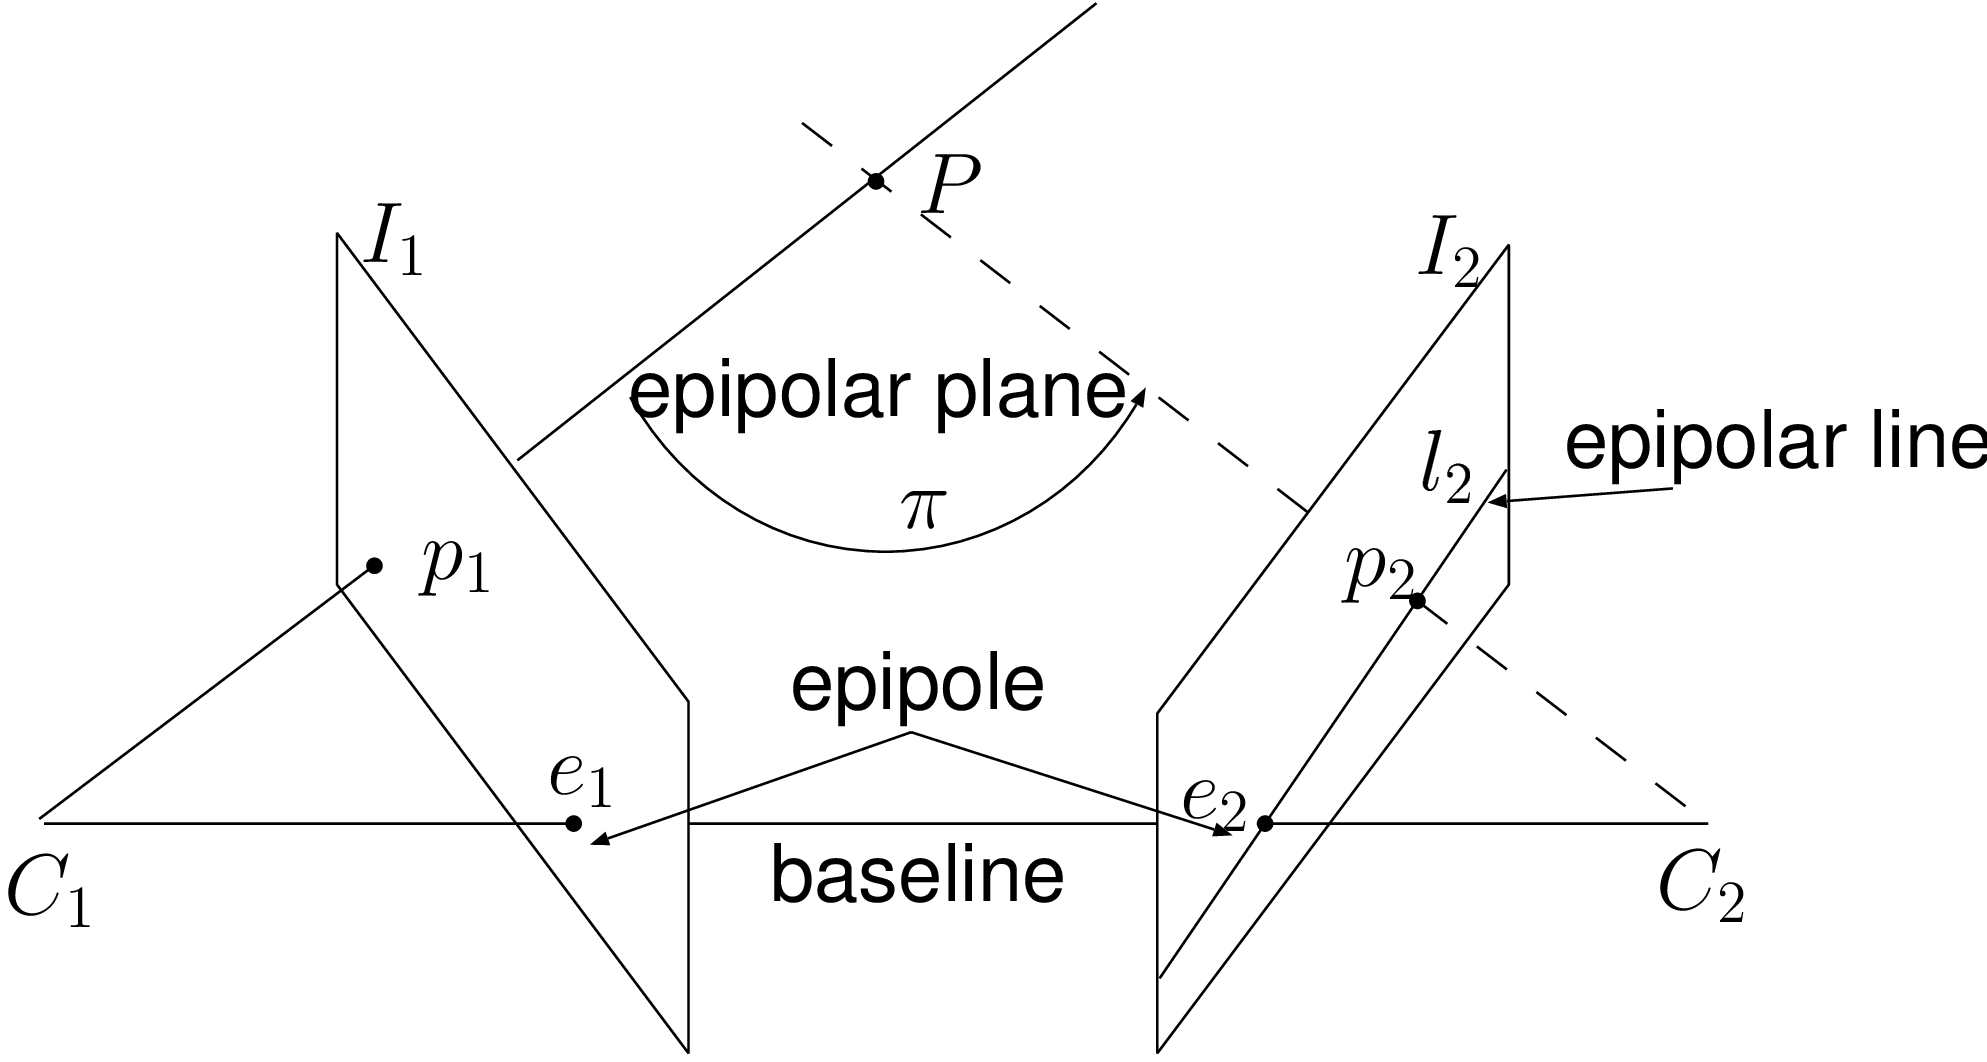
\includegraphics[width=.8\textwidth]{images/epipolar-geometry}}
\caption{Epipolar geometry}
\label{fig:epipolargeom}
	\end{center}
\end{figure}
Main goal of epipolar geometry is the computation of pixels correspondences among the input images. 
Neighbouring pixels information, cameras positions and their calibration data are fundamental to achieve that.
Figure \ref{fig:epipolargeom} demonstrate a pixel in one image $\mathbf{p}_1$ projected to its correspondent epipolar line segment in the other image, which is lower bounded by the projection of the first camera center into the second camera plane, i.e. the epipole $\mathbf{e}_2$. 
Projecting the epipolar line in the second image back to the first, another line would be obtained, bounded by the correspondent epipole $\mathbf{e}_1$. 
The extensions to infinity of these two segment are identified as the epipolar lines, which are defined by the intersection of the two image planes with the epipolar plane.
A fundamental property is that the epipolar plane passes through both camera centers $\mathbf{C}_1$ and $\mathbf{C}_2$, as well as point $\mathbf{P}$. 
Therefore, they lie in the same plane. \\

\subsection{Rectification}
\label{subsection:rectification}
\begin{figure}[t]
	\begin{center}
		{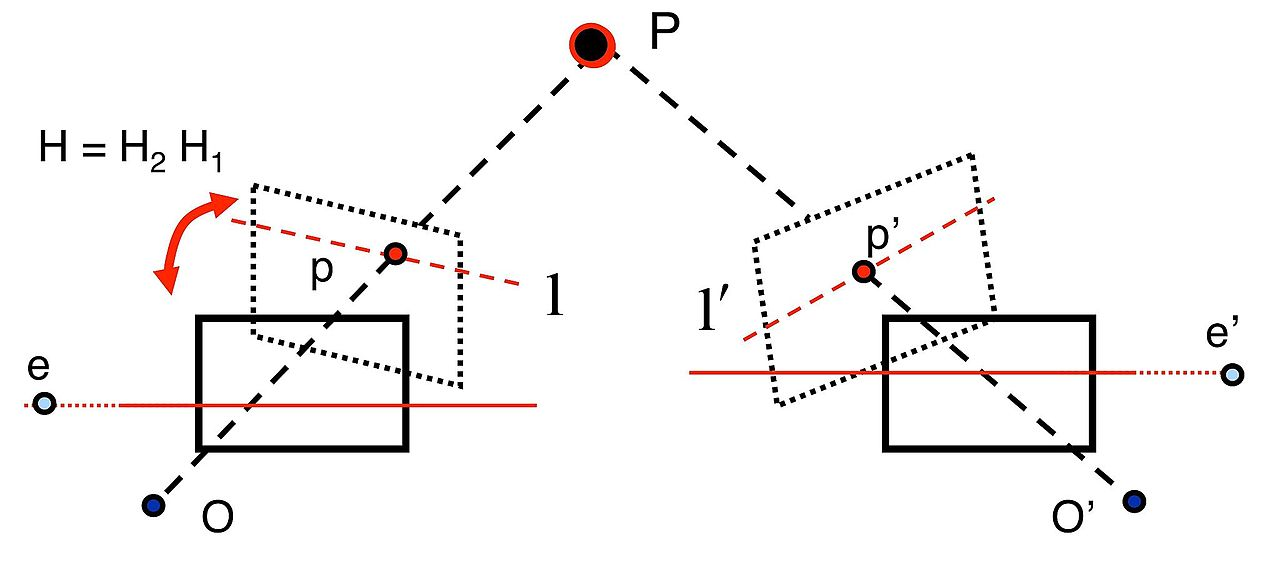
\includegraphics[width=.8\textwidth]{images/rectification}}
\caption{Image rectification -- Source: L. Lebeznik}
\label{fig:rectification}
	\end{center}
\end{figure}

Epipolar geometry for a pair of cameras is relative to pose and calibration of the camera and can be computed using the fundamental matrix, which can be obtained applying the eight point algorithm \citep{hartley2004multiple}.
Computing this geometry allows, then, to find the correspondent pixels between the two images using the constraint of the epipolar lines.
This is possible, because, as explained in \ref{subsection:stereogeom}, considered a pixel in one image, the correspondent one lies on the relative epipolar line.\\
Beside that, pixels correlations can be more efficiently performed by rectifying the input images \citep{hartley2004multiple}.
In Figure \ref{fig:rectification} is clearly visible the outcome of this process and its advantages.
As shown, corresponding horizontal scanlines are epipolar lines. 
The essential importance of this standard rectified geometry is clearly explained by the following equation,
\begin{equation} \label{eqn:disparity-depth}
	d = f \frac{B}{Z}
\end{equation}

that leads to a linear relationship between 3D depth $Z$ and disparity $d$, where $f$ is the focal length (in pixel) and $B$ the baseline.
Moreover, the relationship between the corresponding pixels in the left and right images can be defined as follows:
\begin{equation} \label{eqn:corresponding-pixel}
	x' = x + d(x, y), \; y' = y
\end{equation}

Thus, the main step for recovering a depth image of a scene is the estimation of the disparity map $d(x,y)$.\\
As introduced at the beginning, the best disparity map is estimated after the rectification process. 
This is performed by comparing the similarity of corresponding pixels, as defined in equation \ref{eqn:corresponding-pixel}, and storing them in a disparity space image $C(x,y,d)$, which is then processed with multiple algorithms. 

\subsection{Stereo methods and dense correspondence}
\label{stereomethods}
In this section a brief delineation of the general pipeline implemented in most of the stereo matching method is presented. 
Moreover, as a theoretical completion of what introduced above, some generic algorithm are further explained.\\
Stereo algorithm follows in general a subspace of the following methods: matching cost computation, cost aggregation, disparity computation and optimization and disparity refinement \citep{Scharstein2001}.\\
A preliminary distinction, based on those phases, separates stereo methods between local or window-base global methods.\\
In local methods, the disparity computation in a certain region depends on the pixel intensities within a limited window.\\
On the contrary, global algorithms, are based on an energy function.
In this one smoothness assumptions are defined and then a global optimization problem is solved. 
These algorithm are mainly distinguished considering the minimization strategy, such that, simulated annealing, graph cuts or belief propagation.\\
Between these two classes there are iterative and hierarchical algorithms. 
The latter aim to constraint gradually the disparity estimation from the coarser to the finer levels \citep{Hirschmuller2008}.\\
Considering the first general step of stereo matching algorithms, the matching cost, there are multiple measures to define it.
Among the most prevalent pixel-based algorithm can be included square intensity differences, absolute intensity differences, mean-squared error and mean absolute difference.\\
Other common matching cost comprehend normalized cross-correlation, which is similar to sum-of-squared-difference (SSD), and binary methods. 
However, the latter tend to not be used any longer. \\
On the other hand, lately, more robust algorithms are used for their insensitivity to non-stationary exposure and illumination changes. 
Entropy measures and non-parametric functions such as, rank and census transform \citep{Zabih1994}, sampling insensitive difference\citep{Birchfield1999} and hierarchical mutual information \citep{Hirschmuller2008}, are some examples.
In particular, they allow to obtain accurate performance when considerable exposure or appearance variations are present. \\
Drawing up some conclusion regarding the local methods, the core steps are the matching cost calculation and the aggregation phase. 
Disparity estimation, then, becomes trivial. Each pixel takes the disparity levels whose cost value is the minimum. 
This approach is said to be a local \textit{winner-take-all} optimization. 
A drawback of this approach is that the matches are imposed for the reference image. 
While points is the support image might have multiple correct matches. 
For this reason, cross-checking and post-processing become more relevant here.\\
Summarizing the general pipeline of global stereo matching methods, they often get rid of the aggregation step. 
They usually perform sort of optimization steps after disparity estimation, exploiting the smoothness constraints as aggregation part. \\
Goal of this approach is to find the solution to a global energy function, i.e. the disparity $d$ that minimizes the energy,
\begin{equation}\label{eqn:energyfct}
	E(d) = E_d(d) + \lambda E_s(d)
\end{equation}
where $E_d(d)$ is the data term and $E_s(d)$ the smoothness term.
Adopting the aforementioned disparity space image (DSI) matching cost, the data energy is calculated as:
\begin{equation}\label{dataterm}
	E_d(d) = \sum_{(x,y)} C(x, y, d(x, y))
\end{equation}
where $C$ is the DSI.
Then, the smoothness term is usually defined as:
\begin{equation}\label{smoothterm}
	E_s(d) = \sum_{(x,y)} \rho (d(x,y) - d(x + 1, y)) + \rho (d(x,y) - d(x, y + 1))
\end{equation}
where $\rho$ is some monotonically increasing function of disparity difference. 
For some implementations, the smoothness energy term can also be based on intensity differences,
\begin{equation}\label{smoothtermintensity}
	\rho_d(d(x,y) - d(x + 1, y)) \cdot \rho_I(\Vert I(x,y) - I(x + 1,y) \Vert)
\end{equation}
where $\rho_I$ is a monotonically decreasing function, which depends on the intensity differences and makes the smoothness costs lower at high-intensity gradients.\\
After the energy function has been clearly identified, different categories of algorithms can be exploited to recover a (local) minimum.
Graph cut, belief propagation and Markov random field (MRF) based methods have been proved to give the most accurate results. \\
Mentioning some hybrid methods, there are cooperative algorithms and others based on coarse to fine incremental steps.
Cooperative algorithms were some of the earliest proposed for disparity estimation. They are influenced by human stereo vision processing models. 
They operate by iteratively improve disparity evaluations using non-linear calculations, leading to a result similar to the one of the global methods.
Iterative algorithms are, instead among the current best algorithms.
The main idea is to successively choose the best disparity among all of the possible ones. 
A coarse-to-fine framework is usually used to speed up the computations.\\
Dealing with global optimization methods, it is worth to mention dynamic programming (DP) technique.
Unlike solutions based on equation \ref{eqn:energyfct}, dynamic programming allows to reach global minimum exploiting independent scanlines.
This approach works over a slice of the DSI, i.e. the matching cost cube, finding the path associated to the minimum cost.
The generic implementation of DP along a scanline $y$ and for each input state in a 2D cost matrix $D(m, n)$ leads to combine its DSI value with its previous cost values as follows,
\begin{equation}\label{eqn:dynamicprog}
	C'(m,n) = C(m + n, m - n, y)
\end{equation}
Correct cost selection in presence of occluded pixels and difficulties with scanline consistency are some of the weakness of DP.
Multiple algorithms have been proposed to recover from these problems. 
Scharstein and Szeliski \citep{Scharstein2001} proposed an alternative to standard DP, improving recursively independent scanlines in the global energy function,
\begin{equation}\label{eqn:DPoptimization}
	D(x,y,d) = C(x,y,d) + \min_{d'}\{ D(x - 1, y, d') + \rho_{d} (d - d') \}
\end{equation}
An upgrade of this scanline optimization is the aggregation cost approach used in semi-global matching \citep{Hirschmuller2008}.
In this case, a cumulative cost function is evaluated from at least eight directions.
Intuitively, this approach accesses accurate results and it is highly efficient. \\
Considering more recent improvements to stereo matching, segmentation-based techniques hold a prominent position.
In this case, an initial segmentation of the reference image is performed.
Then, disparities are estimated pixelwise using local methods.
Citing couple of recent approaches, Klaus, Sormann and Karner \citep{Klaus2006} segment the image with mean shift, to get initial disparity estimations. 
Then they apply re-fitting with global planes, and perform final MRF with loopy belief propagation. \\
Wang and Zheng \citep{Wang2008} built a similar top ranked algorithm.
They segment the image with local plane fits. 
Then run cooperative optimization of neighbouring plane fit parameters. 
Others developed similar approaches exploiting color correlation and left-right consistency check for occlusion detection \citep{yang2008stereo} or focusing on alpha mattes fractional pixel extraction \citep{bleyer2009stereo}.\\
As explained in section \ref{sec:problemstat} the area of stereo matching and disparity estimation is one of the most extensively researched topic in computer vision.
Nowadays approaches based on convolutional neural networks and deep learning are going to be the highly ranked in the standard database.
Although, their performance in accuracy tends to decrease a lot when moving from dataset images to real ones.\\
Therefore, novel strategies based on standard stereo geometry algorithms could reach consistent accuracy even in real time \citep{Hernandez-Juarez2016}.
Thus, as described above, after the structure of the cost volume or DSI has been delineated, the actual pixelwise photoconsistency measures are computed.
Multiple methods to achieve this has been proposed during years and already explained in the previous paragraphs.
Then, depth computation is obtained with different form of optimizations. 
These ranges among local, global or hybrid frameworks. \\
Consequently, starting from classical stereo-based methods and building up a novel pipeline, accurate real time depth map estimations can be achieved.
 
\section{Structure of the Thesis}
\label{section:structure} 

You should use transition in your text, meaning that you should help
the reader follow the thesis outline. Here, you tell what will be in
each chapter of your thesis. Often the thesis does not have as many
chapters as is in this template. For example, environment and
implementation can be combined as well as chapters of evaluation and
discussion.  The rest of this thesis is organized as
follows. Chapter~\ref{chapter:background} gives the background, etc.


%
\chapter{Theoretical Background and Related Work}
\label{chapter:background} 

In Chapter~\ref{chapter:intro} a general overview of the project has been proposed and the main purposes of the developed work have been outlined.\\
In this chapter an exhaustive revision of the theoretical basis of most of the stereo-matching methods is presented. 
Then, epipolar geometry, camera calibration and disparity estimation algorithms are specifically described. 
Starting from the necessary mathematical fundamentals, the discussion moves on the disparity estimation algorithms. 
Then, the chapter focus on the main benefits and drawbacks of standard and novel approaches in depths computation.
Comparison between photogrammetry based and deep learning based algorithms is proposed, to provide a clear explanation of the decisions implemented.
At the end a relevant discussion about the main image processing techniques is carried out, thus to analyse some of the algorithms that have been used in the pre and post processing phase of the algorithm. \\
Taking into account the standard algorithms for stereo correspondence, which are mainly based on photogrammetry related operations that fully exploit the mathematical principles of stereo geometry.
They can be conventionally classified into two general categories, local and global approaches~\cite{Scharstein2001}.
Specifically, the local-based methods tend to estimate the disparity image through the analysis of the corresponding pixels between the left and right views of the scene, concerning a particular area. 
Then, the matching cost related to all the potential matches defined for that area is evaluated and employed in the exact disparity estimation.
In order to recover from low accuracy proper of the previous strategies, global-based methods try to calculate the disparity values by minimizing an energy function.
In this context, Semi-Global Matching (SGM) combines strong factors of global and local approaches allowing to obtain a good trade-off between computational cost and accuracy. \\
Technically speaking, SGM applies a pixelwise, Mutual Information (MI) based matching cost for analysing pixel intensity value differences of input images \cite{Hirschmuller2008}.
Moreover, pixelwise matching is enhanced with a smoothness constraint, which leads to a global cost function. 
Then, post-processing techniques are applied to remove outliers and filter the image.\\
Referring to the analysis performed by Scharstein and Szeliski \cite{Scharstein2001}, SGM carries out four main steps, as well as most of the stereo matching algorithms. 
These are defined as: \textit{matching cost computation}, \textit{cost aggregation}, \textit{disparity computation} and \textit{disparity refinement}. \\
Considering the former, it is usually based an absolute, squared or sampling insensitive difference between pixel intensities \cite{Hirschmuller2008}. 
Although those methods allow to reach a reliable accuracy, they are sensitive to radiometric difference. 
Thus, cost based on image gradients or window-based methods, such as Rank and Census transform \cite{Ko2017}, became an optimal choice. 
Furthermore, Mutual Information results as a good trade-off for dealing with complex radiometric relationships between images.\\
In the second phase, cost aggregation accumulate the matching costs coming from multiple directions and along the considered disparity levels. 
Subsequently, disparity evaluation is defined for each pixel, as the one with the lowest cost.
This is the approach typically used for local methods. 
Global algorithms, contrarily, used to get rid of the aggregation step and define a global energy function. 
Over that function, pixel similarity and disparity smoothness are enforced with different strategies. 
In this latter case, the best disparity is identified finding the minimum of the cost function. 
This is achieved with multiple techniques such as: Dynamic Programming (DP) \cite{Birchfield1999}, Belief Propagation \cite{Klaus2006} or Graph Cuts \cite{Kolmogorov2001}.\\
Disparity refinement tends to differ more among the different methods. 
Post-processing techniques such as filtering, outlier removal and consistency check are applied in general.\\
As aforementioned, among the top-ranked stereo matching algorithms, SGM results to be the best performing in terms of computational time and accuracy. 
Its benefits stand in the hierarchical computation of the matching cost, which mainly exploits Mutual Information. 
Cost aggregation is achieved considering a global energy function and a pathwise pixel optimization. 
The final disparity is chosen with a winner takes all strategy. 
Disparity refinement is completed by consistency check between left and right disparity images. \\
Therefore, this brief introduction presents the general concepts of most of the standard stereo matching algorithms.
However, an analysis of the basis of stereo correspondence is equally important in this context, thus to highlight its relevance for multiple applications such as: autonomous driving, robotics, object detection and 3D reconstruction.

\section{Stereo matching and pixel correspondence}
\label{section:stereo-match-and-corr}

First of all, stereo matching is defined as the process of estimating a 3D model of a scene, starting from two or more images. 
Therefore, the matching pixels between the images are found and their 2D positions are converted into 3D depths. 
This procedure and the definition of a dense depth map, generally obtained by assigning the relative depth to the input pixels, is going to be properly described in the following sections.\\
Nonetheless, essential is the concept of disparity, defined as the amount of horizontal motion between two properly configured images of a stereo pair. 
It is inversely proportional to the distance from the observer, i.e. the camera. 
Although these ideas are relatively simple to understand, the challenging task within this process stands in establishing dense and accurate inter-image correspondences \cite{Szeliski2011}.\\
As already underlined, stereo matching is one of the most widely studied topic in computer vision since years and it continues to be one of the most active research in that field. 
In fact, modelling of human visual systems, robotic navigation and manipulation, autonomous driving~\cite{Poggi2019} and 3D model building are only some of the possible applications.\\
Therefore, it worth to explain the fundamental principles of stereo matching, such as epipolar geometry, rectification and disparity map, in order to provide a comprehensive outline of the techniques and the algorithms handled in this project.

\subsection{Concepts of stereo geometry}
\label{subsection:stereo-geometry-basics}

\begin{figure}[t]
	\begin{center}
		{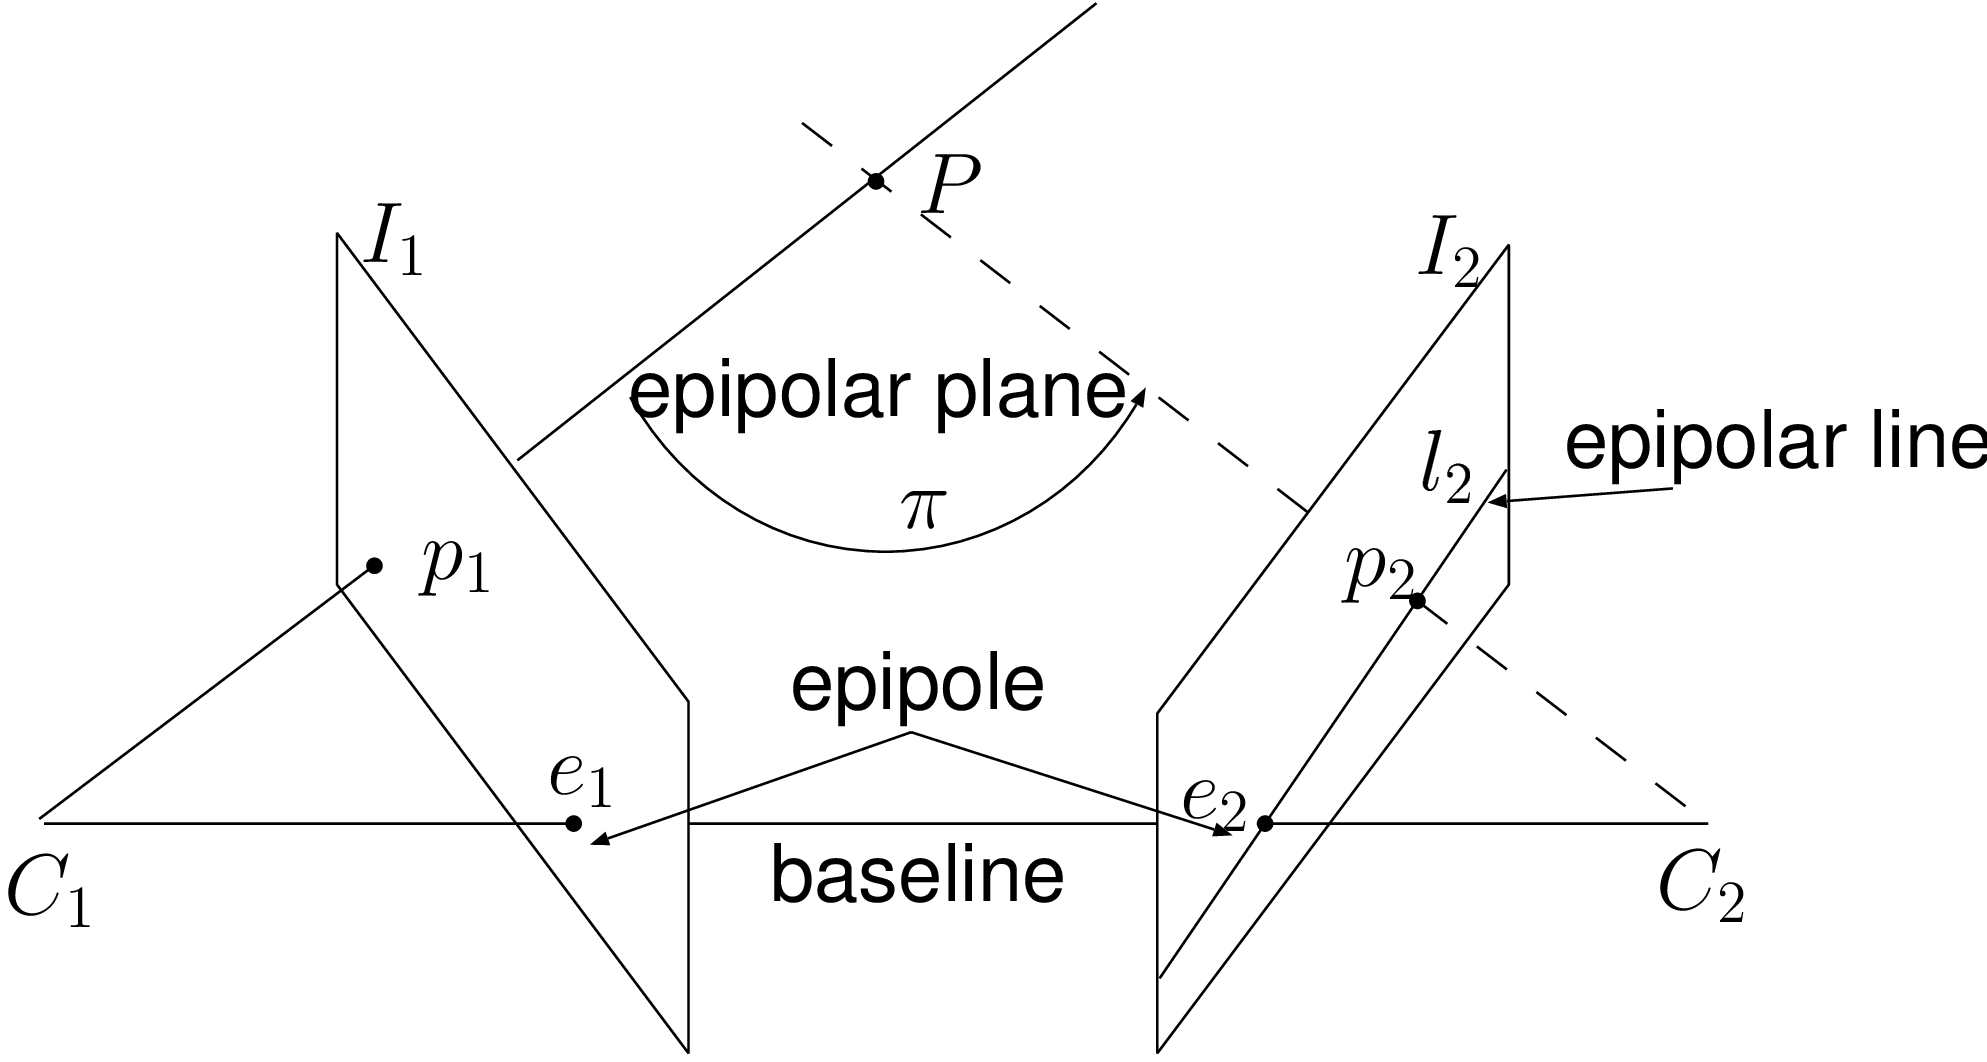
\includegraphics[width=.8\textwidth, height=5cm, keepaspectratio]{images/epipolar-geometry}}
\caption{Epipolar geometry}
\label{fig:epipolargeom}
	\end{center}
\end{figure}

In this section, a generic introduction to the main concepts of stereo geometry is proposed. 
This will be, then, further extended in the following sections, where the different aspects of epipolar geometry and pixel correspondence will be specifically explained.\\
Main goal of epipolar geometry is the computation of pixels correspondences among the input images. 
Neighboring pixels information, cameras positions and their calibration data are fundamental to achieve that.
Figure \ref{fig:epipolargeom} displays a pixel in one image $\mathbf{p}_1$ projected to its correspondent epipolar line segment in the other image, $\mathbf{l}_2$, which is lower bounded by the projection of the first camera center into the second camera plane, i.e. the epipole $\mathbf{e}_2$. 
Projecting the epipolar line in the second image back to the first, another line is obtained, bounded by the correspondent epipole $\mathbf{e}_1$. 
The extensions to infinity of these two segment are identified as the epipolar lines, which are defined by the intersection of the two image planes with the epipolar plane.
A fundamental property is that the epipolar plane passes through both camera centers $\mathbf{C}_1$ and $\mathbf{C}_2$, as well as point $\mathbf{P}$. 
Therefore, they all lie in the same plane.

\subsection{Concepts of rectification}
\label{subsection:rectification-basics}

\begin{figure}[t]
	\begin{center}
		{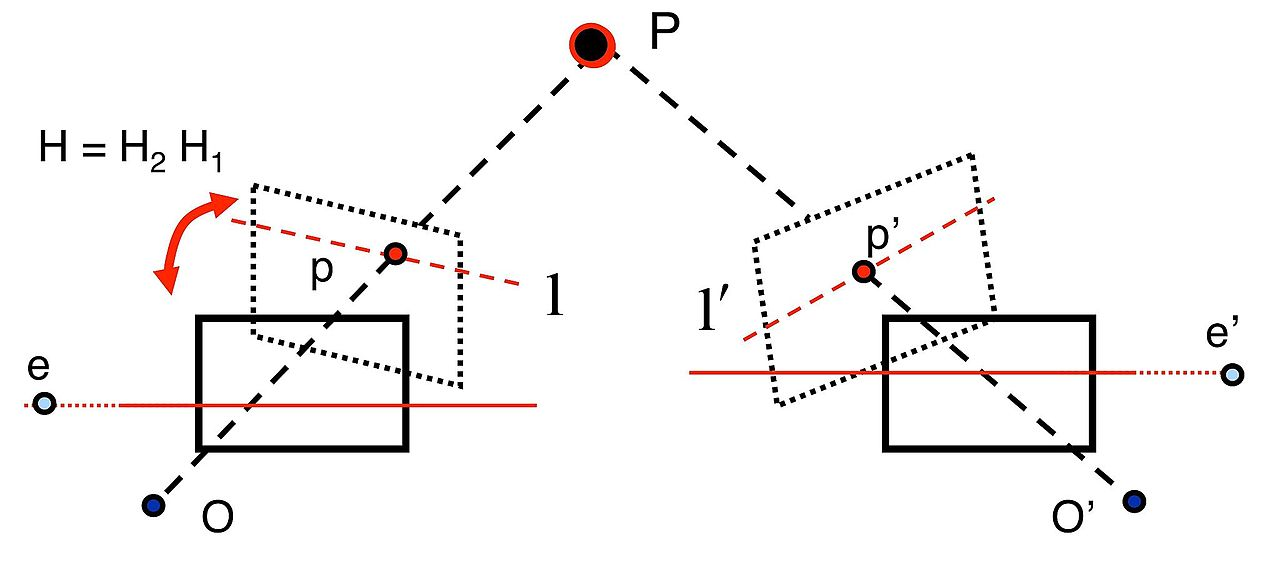
\includegraphics[width=.8\textwidth, height=5cm, keepaspectratio]{images/rectification}}
\caption{Image rectification}
\label{fig:rectification}
	\end{center}
\end{figure}

Epipolar geometry for a pair of cameras is relative to pose and calibration of the camera and can be computed using the fundamental matrix, which can be obtained applying the eight point algorithm \cite{hartley2004multiple}.
This geometry allows, then, to find the correspondent pixels between the two images using the constraint of the epipolar lines.
This is possible, because, as explained in \ref{subsection:stereo-geometry-basics}, considered a pixel in one image, the correspondent one lies on the relative epipolar line, in the other image plane.\\
Beside that, pixels correlations can be more efficiently performed by rectifying the input images \cite{hartley2004multiple}.
In Figure \ref{fig:rectification} is clearly visible the outcome of this process and its advantages.
In fact, it is not difficult to notice that corresponding horizontal scanlines are epipolar lines. 
The essential importance of this standard rectified geometry is clearly explained by the following equation,

\begin{equation} 
\label{eqn:disparity-depth}
	d = f \frac{B}{Z}
\end{equation}

that leads to a linear relationship between 3D depth $Z$ and disparity $d$, where $f$ is the focal length (in pixel) and $B$ the baseline.
Moreover, the relationship between the corresponding pixels in the left and right images can be defined as follows:

\begin{equation} 
\label{eqn:corresponding-pixel}
	x' = x + d(x, y), \; y' = y
\end{equation}

Thus, the main step for recovering a depth image of a scene is the estimation of the disparity map $d(x,y)$.\\
As introduced at the beginning, the best disparity map is estimated after the rectification process. 
This is performed by comparing the similarity of corresponding pixels, as defined in equation~\ref{eqn:corresponding-pixel}, and storing them in a disparity space image (DSI)~\cite{yang1993local}, in general labelled with $C(x,y,d)$, which is then processed with multiple algorithms. 
Specifically, the concept of DSI can be described as any image or function established over a continuous or discretized representation of a disparity space $(x, y, d)$.
Basically, it denotes the cost, as log likelihood or confidence measure, of a specific match related to $d(x, y)$.
Therefore, the main task of any stereo matching algorithm is to determine the specific surface included in the DSI that has some optimal property, as can be lowest cost and finest smoothness.
This procedure can be more simply described as the finding of the univalued function, contained in $d(x, y)$, that best approximate the structure of the surfaces in the scene.

\section{Epipolar geometry and Rectification}
\label{sec:eipolarandrect}

Fundamental problem of stereo vision is the estimation of 3D locations of points from at least two corresponding input images.
This process, which comprises concurrent computation of both 3D geometry and camera pose, is generally known as structure from motion~\cite{Szeliski2011}.\\
In the explanation of these topics it is necessary to start discussing about the triangulation.
Then, the concept of epipolar geometry is outlined and after that the notions of camera calibration and rectification. 

\subsection{Triangulation}
\label{subsection:triangulation}

\begin{figure}[t]
	\begin{center}
		{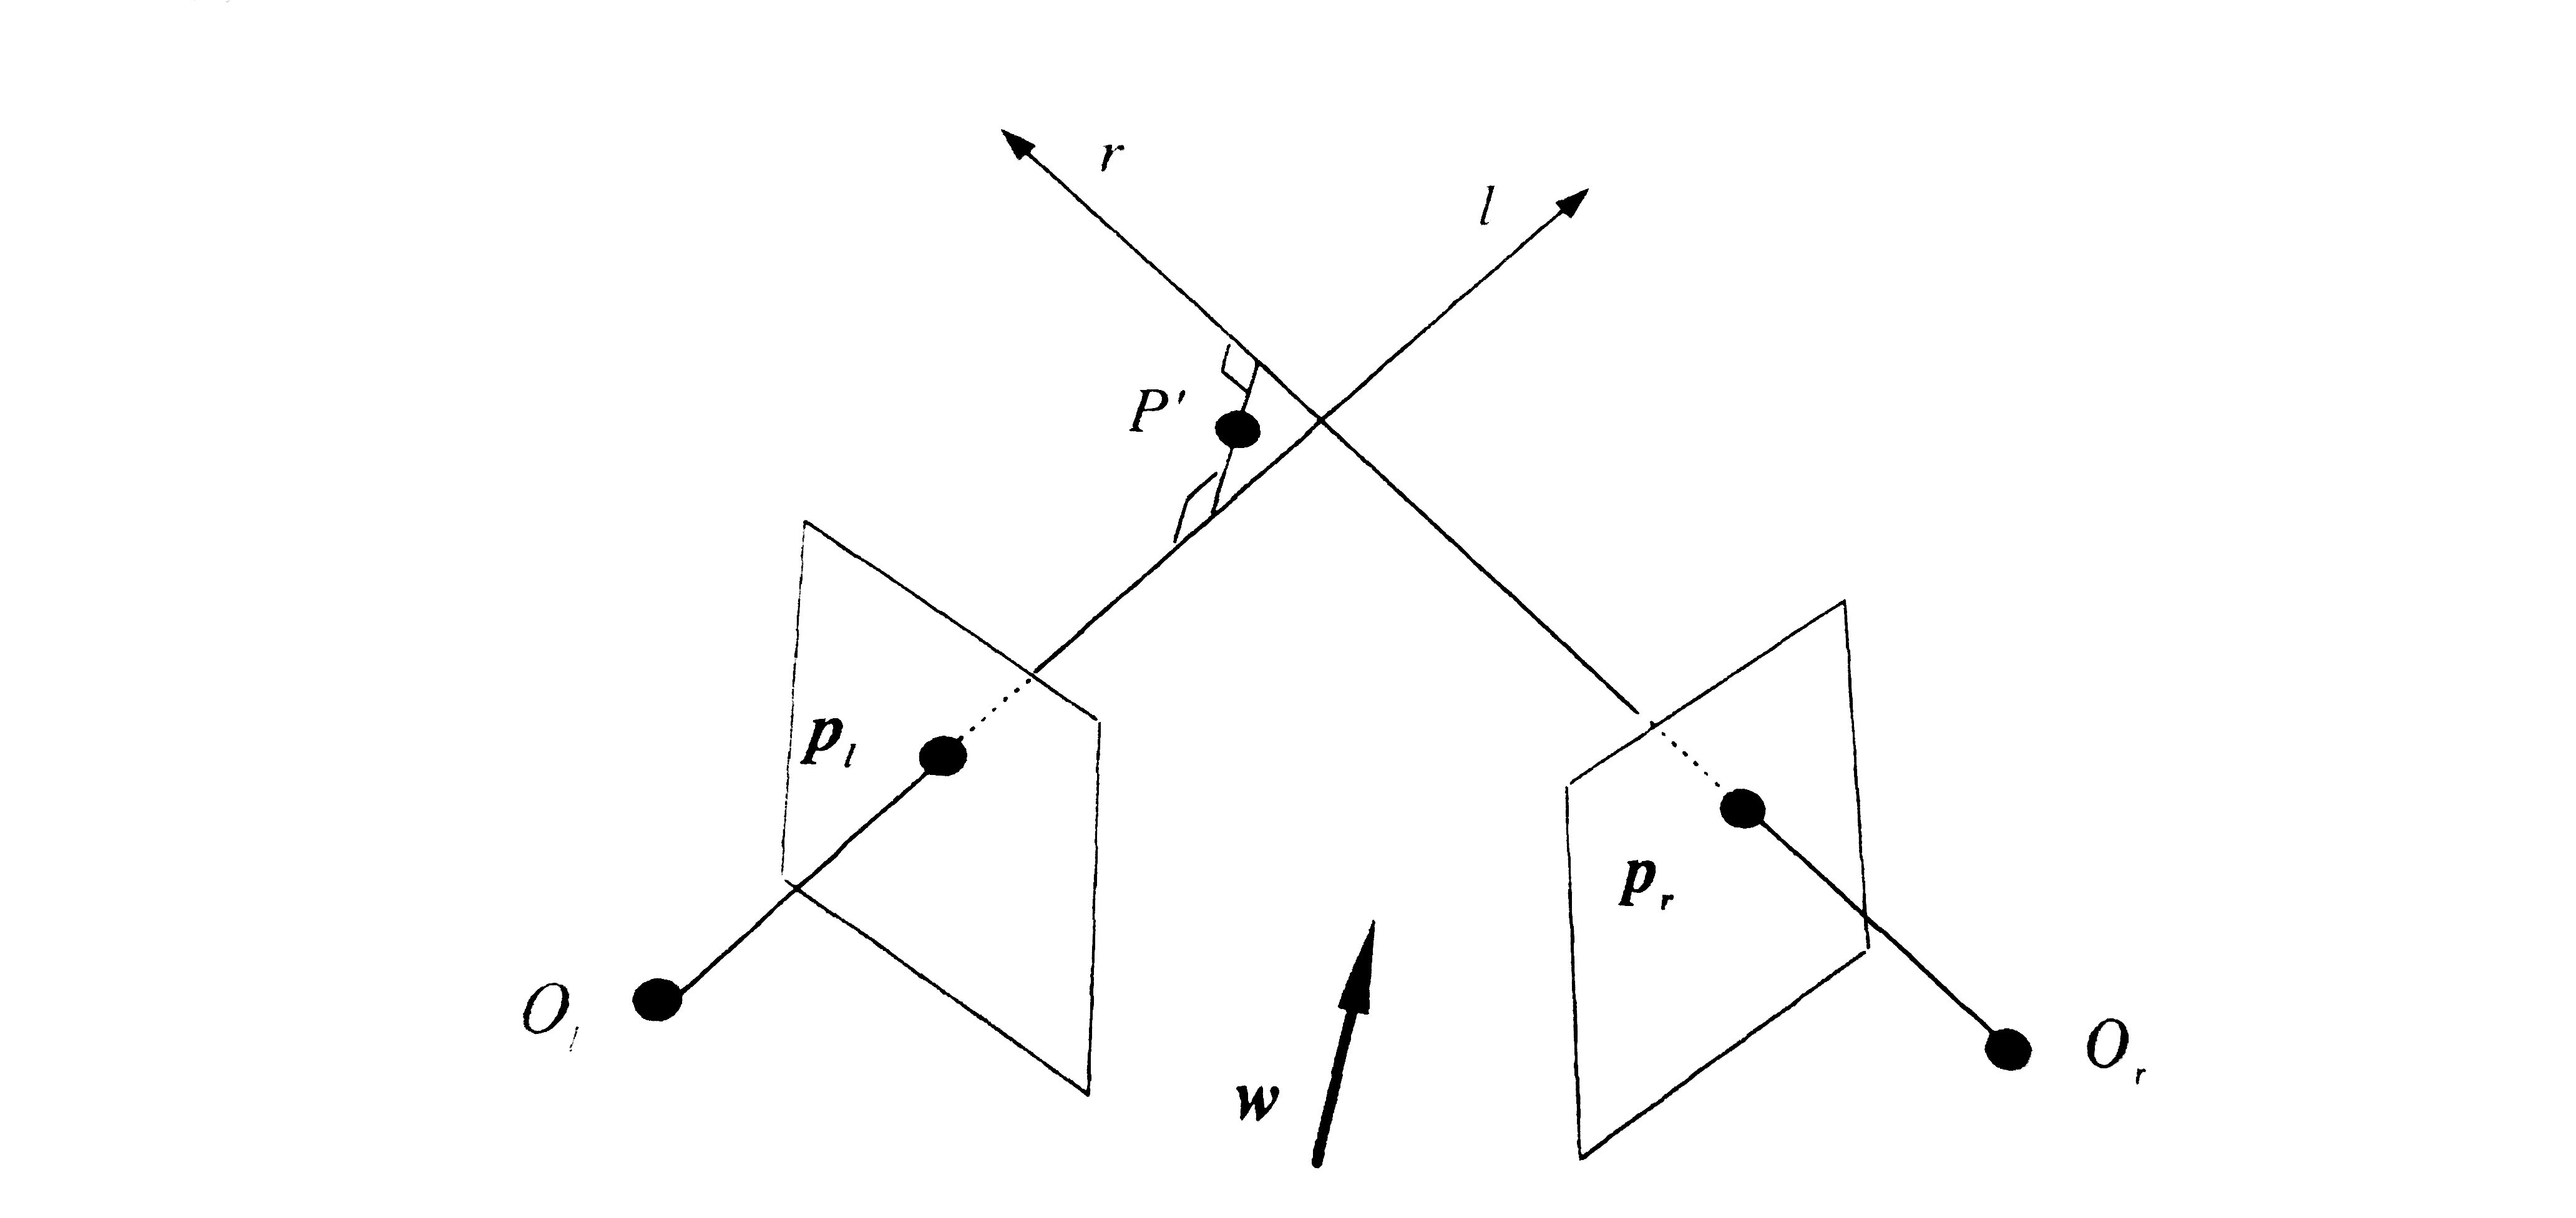
\includegraphics[width=.8\textwidth, height=5cm, keepaspectratio]{images/triangulation}}
\caption{3D triangulation by finding point $P'$ that lies nearest to all of the optical rays}
\label{fig:triangulation}
	\end{center}
\end{figure}

Triangulation is the problem of detecting 3D point positions from a collection of corresponding 2D image locations, assuming that camera poses are known.
Figure~\ref{fig:triangulation} shows one of the easiest methods to tackle this problem. 
Objective is to evaluate the 3D position of $P'$ that have the smallest error to all of the 3D optical rays coming from the camera centers, which identify the 2D point locations in the image plane, i.e. $P_r$ and $P_l$.
As shown in Figure~\ref{fig:triangulation}, the rays starts from the camera centers, $O_l$ and $O_r$, and go in direction of $l$ and $r$, which can be defined using the camera matrix, usually identified with $ P_j = K_j [ R_j | t_j ] $.
The closest point to $P$ on this ray minimizes the distance,

\begin{equation}
\label{eqn:mindist}
	\Vert O_j + d_j \hat{v}_j - P \Vert^2
\end{equation}

Therefore, because of the minimum is $d_j = \hat{v}_j \cdot (p - c_j)$, the nearest points are calculated as:

\begin{equation}\label{eqn:closestpoint}
	q_j = O_j + (\hat{v}_j \hat{v}_j^\top)(P - O_j) = O_j + (P - O_j)_{\Vert}
\end{equation}

Hence, the optimal value for $P$, obtained solving a least square problem, becomes,

\begin{equation}\label{eqn:solP}
	P = \Big[ \sum_j (I - \hat{v}_j \hat{v}_j^\top ) \Big]^{-1} = \Big[ \sum_j (I - \hat{v}_j \hat{v}_j^\top )O_j \Big]
\end{equation}

\subsection{Epipolar geometry}
\label{subsection:epipolar-geometry}

\begin{figure}[t]
	\begin{center}
		{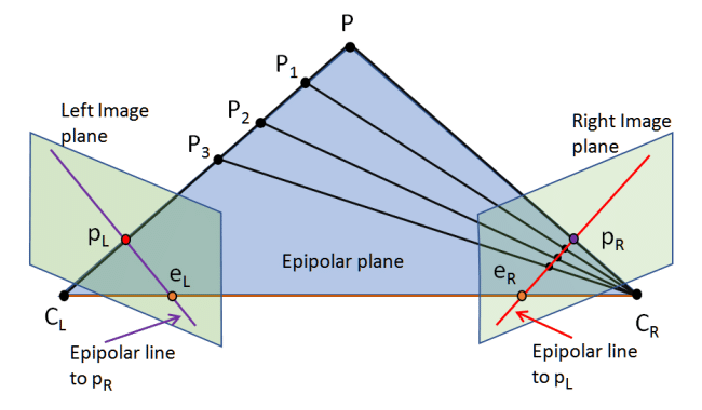
\includegraphics[width=.8\textwidth, height=5cm, keepaspectratio]{images/epipolar-geometry-2}}
\caption{Epipolar geometry. Image point $p_L$ back-projects to a ray in a 3D space defined by $C$ and $p_L$. This ray becomes a line, the epipolar line to $p_L$, in the second view. The image of $P$, i.e. $p_R$, must lie on this line}
\label{fig:epipolargeom-2}
	\end{center}
\end{figure}

The intrinsic projective geometry between two views is known as epipolar geometry.
It is only dependent on the cameras' internal parameters and pose.
The $3 \times 3$ rank 2 matrix that defines this geometry is the fundamental matrix $F$.\\
The epipolar geometry is the basis for finding corresponding points in stereo matching. 
It is basically defined by the intersection between image planes and the one on which the cameras baseline lies.\\
A fundamental property, that makes this geometry extremely useful, is that image points, space point and camera centers are coplanar. 
Considering Figure~\ref{fig:epipolargeom-2} and assuming that only $p_L$ is known, that geometry allows to constraint the corresponding point $p_R$. 
The epipolar plane is defined by the baseline and the ray that comes from $p_L$. 
Hence, knowing that $p_R$ lies on the same plane, that point belongs to $l_R$, i.e. the intersection between the epipolar plane and the second image plane, knows as the epipolar line to $p_L$.
Therefore, exploiting this property, the searching of corresponding points is constrained to only one line inside the image.\\
Mathematical definition of the epipolar geometry is the fundamental matrix $F$.
As already demonstrated through Figure~\ref{fig:epipolargeom-2}, for each point $p_L$ in one image, the corresponding epipolar line $l_R$ to that point belongs to the other image plane. 
Moreover, any point $p_R$ in the second image, which is related to point $p_L$, lies on $l_R$.
Hence, the epipolar line is described as the projection in the second image of the ray that comes from the point in the first image, passing through its camera center.
This defines a map, $p_L \rightarrow l_R$, which relates the points in one image with the corresponding epipolar lines in the second image.
This correlation, between points and lines, is represented by the fundamental matrix $F$.\\
Considering the aforementioned map $p_L \rightarrow l_R$ described by $F$, an important property of the fundamental matrix is defined,

\begin{equation}
\label{eqn:fundmatprop}
	p_R^\top F p_L = 0
\end{equation}

Therefore, assuming two corresponding points $p_L$ and $p_R$, it is known that $p_R$ lies on the epipolar line $l_R = F p_L$. 
Thus, the mathematical correlation is,

\begin{equation}
	0 = p_R^\top l_R = p_R^\top F p_L
\end{equation}

Reciprocally, if image points comply the relation \ref{eqn:fundmatprop}, then the rays identified by these points are coplanar. 
For corresponding points this is a necessary condition.
Equation \ref{eqn:fundmatprop} is extremely important because it allows to characterize the fundamental matrix without reference to the camera matrices \cite{hartley2004multiple}.
Thus, using at least 7 correspondences, it is possible to recover the fundamental matrix $F$. 
This estimation is known as \textit{weak calibration}.\\

\subsection{Rectification}
\label{subsection:rectification}

As introduced in section~\ref{subsection:rectification-basics}, image rectification is defined as the process of obtaining a pair of \textit{matched epipolar projections} from a pair of stereo images, which are taken from generally differing viewpoints.
In the rectified projections the epipolar lines become parallel with respect to the x-axis. 
Thus, they match between the stereo pair and so the disparities are in the x-direction only.\\
In order to obtain a rectified stereo pair, 2D projective transformations are employed to the images, so that the epipolar lines can match.
Using this method, the transformations are built up in a way that the corresponding points have almost the same x-coordinate.
Actually, this strategy leads to a minimal distortion on the images, being the two transformations arbitrary. 
However, working on rectified images, the matching problem is highly simplified, being correlated only to epipolar geometry and near-correspondence. \\
Core problem of this section is to find the appropriate projective transformation $H$. 
Indeed, to get epipolar lines parallel with x-axis, the epipole should be mapped to an infinite point. 
This, has to be done correctly, otherwise intensive projective distortion of the image can happen.
For this reason, constraints are set on the definition of $H$.\\
First of all, restricting $H$ to be a rigid transformation in the neighborhood of a given point\footnote{this means that to first-order, the neighbourhood of the point may be subjected to rotation and translation only}, the errors are reduced.\\
Once the epipole has been mapped to infinity, it is then necessary define a map to match the corresponding epipolar lines.
This resampling is build up in such a way that, being $l_L$ and $l_R$ any pair of epipolar lines, then,

\begin{equation}
	H^{-\top} l_L = H'^{-\top} l_R
\end{equation}

Satisfying the condition above, a matched pair of transformations is recovered.\\
Specifically, at first $H'$ is chosen, so that it can map the epipole $e_R$ to infinity. 
Then the matching transformation $H$ is defined minimizing the sum-of-square distances,

\begin{equation}
\label{eqn:match-transf-constr}
	\sum_i d(H p_{L_i}, H'p_{R_i})^2
\end{equation}

Therefore, the full algorithm can be summarized as follows.\\
The outcome of this resampling process is a pair of stereo images whose epipolar lines are horizontal.
Hence, the disparities are calculated along the epipolar lines. 
First of all, at least seven corresponding matches are defined.
This allows to compute the fundamental matrix $F$, applying the so called eight-point algorithm, and after that the two epipoles are found.
After that, there is the selection of the projective transformation $H'$, that maps the epipole of the support image to infinity.
The corresponding transformation $H$ is found solving the least-square problem.
Finally both of the input images are resampled according to $H$ and $H'$.

\section{Standard stereo methods and dense correspondence}
\label{section:stereo-methods}

In this section a brief delineation of the general pipeline implemented in most of the stereo matching method is presented. 
Moreover, as a theoretical completion of what introduced above, some generic algorithms are further explained.

\subsection{Standard stereo matching algorithms}
\label{subsection:standard-methods}

Standard stereo matching algorithm follows in general a subspace of the following methods: matching cost computation, cost aggregation, disparity computation and optimization and disparity refinement \cite{Scharstein2001}.\\
A preliminary distinction, based on those phases, separates stereo methods between local or window-base and global methods.\\
In local methods, the disparity computation depends on the pixel intensities within a limited window, considering a specific region of the image.\\
On the contrary, global algorithms, are based on an energy function.
In the latter smoothness assumptions are defined and then a global optimization problem is solved. 
These algorithm are mainly distinguished considering the minimization strategy, such that, simulated annealing, graph cuts or belief propagation.\\
Between these two classes there are iterative and hierarchical algorithms. 
The latter aim to constraint gradually the disparity estimation from the coarser to the finer level \cite{Hirschmuller2008}.\\
Considering the first general step of stereo matching algorithms, the matching cost, there are multiple measures to define it.
Among the most prevalent pixel-based algorithm can be included square intensity differences, absolute intensity differences, mean-squared error and mean absolute difference.\\
Other common matching cost comprehend normalized cross-correlation, which is similar to sum-of-squared-difference (SSD), and binary methods, which, however, tend to not be used any longer. \\
On the other hand, more robust algorithms are generally used for their insensitivity to non-stationary exposure and illumination changes. 
Entropy measures and non-parametric functions such as, rank and census transform \cite{Zabih1994}, sampling insensitive difference\cite{Birchfield1999} and hierarchical mutual information \cite{Hirschmuller2008}, are some examples.
In particular, they allow to obtain accurate performance when considerable exposure or appearance variations are present. \\
Drawing up some conclusion regarding the local methods, the core steps are the matching cost calculation and the aggregation phase. 
Disparity estimation, then, becomes trivial. 
Each pixel takes the disparity level whose cost value is the minimum. 
This approach is said to be a local \textit{winner-take-all} optimization. 
A drawback of this approach is that the matches are imposed for the reference image. 
While points in the support image might have multiple correct matches. 
For this reason, cross-checking and post-processing become more relevant here.\\
Summarizing the general pipeline of global stereo matching methods, they often get rid of the aggregation step. 
They usually perform some sort of optimization steps after disparity estimation, exploiting the smoothness constraints as aggregation part. \\
Goal of this approach is to find the solution to a global energy function, i.e. the disparity $d$ that minimizes the energy,

\begin{equation}
\label{eqn:energyfct}
	E(d) = E_d(d) + \lambda E_s(d)
\end{equation}

where $E_d(d)$ is the data term and $E_s(d)$ the smoothness term.
Adopting the definition of disparity space image (DSI) matching cost, introduced in Section~\ref{subsection:rectification-basics}, the data energy is calculated as:

\begin{equation}
\label{eqn:dataterm}
	E_d(d) = \sum_{(x,y)} C(x, y, d(x, y))
\end{equation}

where $C$ is the DSI.
Then, the smoothness term is usually defined as:

\begin{equation}
\label{eqn:smoothterm}
	E_s(d) = \sum_{(x,y)} \rho (d(x,y) - d(x + 1, y)) + \rho (d(x,y) - d(x, y + 1))
\end{equation}

where $\rho$ is some monotonically increasing function of disparity difference. 
For some implementations, the smoothness energy term can also be based on intensity differences,

\begin{equation}
\label{eqn:smoothtermintensity}
	\rho_d(d(x,y) - d(x + 1, y)) \cdot \rho_I(\Vert I(x,y) - I(x + 1,y) \Vert)
\end{equation}

where $\rho_I$ is a monotonically decreasing function, which depends on the intensity differences and makes the smoothness costs lower at high-intensity gradients.\\
After the energy function has been clearly identified, different categories of algorithms can be exploited to recover a (local) minimum.
Graph cut, belief propagation and Markov random field (MRF) based methods have been proved to give the most accurate results. \\
Mentioning some hybrid methods, there are cooperative algorithms and others based on coarse to fine incremental steps.
Cooperative algorithms were some of the earliest proposed for disparity estimation. 
They are influenced by human stereo vision processing models. 
They operate by iteratively improve disparity evaluations using non-linear calculations, leading to a result similar to the one of the global methods.
Iterative algorithms are among the current best algorithms.
The main idea is to successively choose the best disparity among all of the possible ones. 
A coarse-to-fine framework is usually used to speed up the computations.\\
Dealing with global optimization methods, it is worth to mention dynamic programming (DP) technique.
Unlike solutions based on equation~\ref{eqn:energyfct}, dynamic programming allows to reach global minimum exploiting independent scanlines.
This approach works over a slice of the DSI, i.e. the matching cost cube, finding the path associated to the minimum cost.
The generic implementation of DP along a scanline $y$ and for each input state in a 2D cost matrix $D(m, n)$ leads to combine its DSI value with its previous cost values as follows,

\begin{equation}
\label{eqn:dynamicprog}
	C'(m,n) = C(m + n, m - n, y)
\end{equation}

Correct cost selection in presence of occluded pixels and difficulties with scanline consistency are some of the weakness of DP.
Multiple algorithms have been proposed to recover from these problems. 
Scharstein and Szeliski~\cite{Scharstein2001} proposed an alternative to standard DP, improving recursively independent scanlines in the global energy function,

\begin{equation}
\label{eqn:DPoptimization}
	D(x,y,d) = C(x,y,d) + \min_{d'}\{ D(x - 1, y, d') + \rho_{d} (d - d') \}
\end{equation}

An upgrade of this scanline optimization is actually the aggregation cost approach used in SGM method \cite{Hirschmuller2008}.
In this case, a cumulative cost function is evaluated from at least eight directions.
Intuitively, this approach accesses accurate results and it is highly efficient. \\
Considering more recent improvements to stereo matching, segmentation-based techniques hold a prominent position.
In this case, an initial segmentation of the reference image is performed.
Then, disparities are estimated pixelwise using local methods.
Citing couple of recent approaches, Klaus, Sormann and Karner \cite{Klaus2006} segment the image with mean shift, to get initial disparity estimations. 
Then they apply re-fitting with global planes, and perform final MRF with loopy belief propagation. \\
Wang and Zheng \cite{Wang2008} built a similar top ranked algorithm.
They segment the image with local plane fits. 
Then run cooperative optimization of neighboring plane fit parameters. 
Others developed similar approaches exploiting color correlation and left-right consistency check for occlusion detection \cite{yang2008stereo} or focusing on alpha mattes fractional pixel extraction \cite{bleyer2009stereo}.\\
As explained in section \ref{section:stereo-match-and-corr} the area of interest for stereo matching and disparity estimation is one of the most extensively researched topic in computer vision.
Nowadays approaches based on Convolutional Neural Networks (CNNs) and deep learning are going to be the highest ranked in the standard database.
Although, their performance in accuracy tends to decrease a lot when moving from dataset images to real ones.\\
Therefore, novel strategies based on standard stereo geometry algorithms could reach consistent accuracy even in real time \cite{Hernandez-Juarez2016}.
Thus, as described above, after the structure of the cost volume or DSI has been delineated, the actual pixelwise photoconsistency measures are computed.
Multiple methods to achieve this has been proposed during years and already explained in the previous sections.
Then, depth computation is obtained with different form of optimizations. 
These ranges among local, global or hybrid frameworks. \\
Consequently, starting from classical stereo-based methods and building up a novel pipeline, accurate real time depth map estimations can be achieved.

\subsection{Deep learning based methods}
\label{subsection:deep-learn-meth}

Considering that disparity estimation from a rectified stereo pair is still one of the most important tasks in computer vision, the latest years have seen an important development of deep learning based methods. \\
Usually these approaches comprises a main pipeline, based on a standard local or global method, whose parameters are finely tuned exploiting Convolutional Neural Networks (CNNs). 
Therefore, in most of the cases, Semi Global Matching (SGM) is used as regularization method, because of its accuracy and relatively low computational time. 
Then, deep learning based methods are used for tuning the penalty parameters, which are related to smoothness and discontinuity of the disparity map. 
As described above, those penalties are empirically adjusted in the standard methods. 
Therefore, the CNNs based approach aims at learn the penalties, in correlation with the 3D structure of the objects in the scene, to achieve an improvement in the disparity map. \\
As aforementioned, several of these deep learning approaches has been proposed in the latest years, and some of them has been able to reach state-of-the-art level of accuracy on the KITTI datasets~\cite{menze2015object}.\\
Even though these method suffer drop in accuracy when shifting from synthetic to real images, it is worth to describe some of them, which are ranked among the state of the art methods in the KITTI benchmark. \\
Seki and Pollefeys proposed \textbf{SGM-Nets}~\cite{Seki2017}, a CNNs based method for penalty estimation, which exploit SGM as regularization technique in the main pipeline. 
They used small image patches and their locations as inputs to the network to predict penalties for the 3D object structures. 
Actually, they developed a novel loss function for training the network, whose inputs are small image patches and their related positions. 
Moreover, they managed to separate positive and negative disparity changes, thus to retrieve object structures more discriminatively.\\
More in detail, SGM-Net produces $P_1$ and $P_2$, which are the specific penalty values generally used in the aggregation cost phase of the standard SGM pipeline, for each pixel. 
This is achieved though a training and a testing phase. 
In the former, the network is iteratively trained by minimizing a \textit{Path cost} and a \textit{Neighbor Cost}. 
In testing, the standard SGM pipeline is run using the penalties estimated by the network. 
Actually, the \textit{Path Cost} is how the authors of the paper called the loss function that they developed, which they minimized using forward and back propagation.
Moreover, they introduced the \textit{Neighbor cost} function for removing the ambiguous disparities traversed along each path, which can lead to wrong penalties.\\
Another approach similar to the one just described is the method developed by Kuzmin et al.~\cite{Kuzmin2017}. 
The core of their method is the prediction of the local parameters of cost volume aggregation process, which they perform exploiting a deep convolutional network. 
Thus, as in \cite{Seki2017}, they avoid to apply deep learning of pixel appearance descriptors, using classical matching scores instead. 
Thus, they refuse learning high dimensional descriptors and matching them, as it used to happen in most of the first deep learning based algorithms.
On the contrary, they focus the learning on the cost-aggregation step. 
Thus, they defined the overall matching cost using a combination of Census transform and sum-of-absolute-differences (SAD). 
Then, they carry out the cost-aggregation phase, which is peculiar for smoothing the general matching cost and correct the wrong matches, applying the domain transform (\cite{Gastal2011},\cite{Pham2013}).
Basically, they develop a deep CNN to estimate on a pixel basis the cost-aggregation parameters and make them spatially varying. 
In this way, they were able to have smoother disparities on the same object and avoid smoothing across object boundaries. 
Therefore, combining standard methods for the matching cost and applying end-to-end deep learning process to the cost-aggregation step, they obtain state-of-the-art accuracy in the KITTI 2015 dataset. 
Differently from \cite{Zbontar2016}, \cite{Zbontar2015} and similarly to \cite{Mayer2016}, they build up an end-to-end learning method that comprises all the part of depth map computation in it. 
Furthermore, unlike \cite{Mayer2016}, their approach exploits classical stereo matching techniques as modules within a more complex neural network structure. 
Their process encompasses the definition of a general cost volume, the cost-aggregation step over that volume and the final winner-takes-all label selection. 
Then, left-right consistency and filling of occluded pixels are performed as post-processing.\\
A different approach with respect to the previous one stands in the implementation developed by \^{Z}bontar and LeCun~\cite{Zbontar2016}.
They focus their attention on the matching cost computation, which is usually the first step of a stereo matching algorithm. 
They developed their method using a CNN to learn similarity measures on small image patches. 
Specifically, they structure the training in a supervised manner building up a binary classification data set with examples of similar and dissimilar pairs of patches. 
Moreover, they carry out two different architectures, one adjusted for speed, and another one for accuracy. 
Thus, the output of the network handles the initialization of the stereo matching cost. 
After that, post processing steps are applied: cross-based cost aggregation, semi-global matching and finally disparity refinement techniques such as, left-right consistency check, subpixel enhancement, median and bilateral filters.\\
Technically speaking, they present a network that is trained on pairs of small image patches, for which the disparity value is known. 
Then, they initialize the matching cost using the output of the network.
After that, they propose a series of common post-processing steps, which are though crucial to obtain accurate results.
Cross-based cost aggregation is exploited for combining matching cost between neighbouring pixels with similar intensities. 
Then, constraints are enforced for smoothness and left-right consistency check applied for detect and eliminate errors in occluded regions. 
The final disparity map is then obtained applying median and bilateral filters, useful for subpixel enhancement. \\
Related problems to \cite{Zbontar2016} are the works by Haeusler et al.~\cite{Haeusler2013} and by Spyropoulos et al.~\cite{Spyropoulos2014}. 
Using a similar approach, they concentrate their attention on predicting the confidence of the calculated matching cost. 
Specifically, in \cite{Haeusler2013}, the aim was using a random forest classifier to connect multiple confidence measures. 
Similarly, the authors of \cite{Spyropoulos2014} focused in estimating the confidence of the matching cost by training a random forest classifier. 
Then, they employed the predictions as mild constraints in a Markov Random Field (MRF) aiming at reducing the errors of the stereo method.\\
Focusing on confidence prediction intended at the estimation of dense disparity map, it is worth to cite the work of \cite{Seki2016}.
They adopted two channels disparity patches as inputs of a CNN, predicting the correctness of stereo correspondences, that is the confidence. 
Using these specific patches, they managed to simultaneously train features and classifiers.
Furthermore, they incorporate the predicted confidence into SGM, adjusting its parameters directly. \\
Unlike methods based on hand crafted features, which lead to limited accuracy, authors of \cite{Seki2016} leverage CNNs to overcome that problem. 
In fact, CNNs support high performance from low level processing, such as patch based matching, to high level, like scene classification and object detection. \\
Therefore, as previously stated, they conceive a two channels disparity patch, based on the concept of standard confidence features.
Then they apply those patches as input to the network, obtaining a simultaneous training of discriminative features and classifiers.
Moreover, they also developed three different types of network structures to manage the trade-off between computational time and accuracy. 
Finally, the confidence was combined into SGM, so that dense disparity map can be obtained.

\subsubsection{Confidence measures}
\label{subsection:conf-measure}

Considering some of the deep learning based methods described in Section~\ref{subsection:deep-learn-meth}, becomes necessary to define the main typology of elements proposed during the years to estimate the confidence of stereo correspondences. \\
Because of many features were introduced by different works in computer vision field, Hu and Mordohai~\cite{Hu2012} developed a broad evaluation of them, leading to the definition of five groups, used for categorize those characteristics. \\
The first group is correlated to the matching cost. 
This means that correct correspondence are unlike to be connected to large matching costs. 
The second group focuses on local properties of the cost curve. 
That is, confidence measure becomes the curvature around the minimum matching cost. 
For example, flat curves, which have smaller values, and describe texture-less areas, express higher ambiguity.
Features related to local minima of the cost curve form the third group. 
As an example, the so called \textit{Peak Ratio (PKR)}, is calculated as the minimum matching cost divided by the second local minima.
Then, a probability mass function over disparity defined using the entire cost curve describes the fourth group.
The last group includes features that highlight the consistency between left and right disparity map, i.e. correct matches indicate more consistent disparity.\\
A similar but more recent work is the one carried out in \cite{Poggi2017} driven by the deep learning breakthrough lately happened in the computer vision area. 
In fact, changes such as, availability of bigger and more challenging datasets, novel and more accurate stereo algorithms and confidence measures, leverage techniques based on deep learning.
Therefore, the authors of \cite{Poggi2017} focus on implement a complete and updated quantitative analysis of the state-of-the-art confidence measures.\\
As a matter of fact, after the analysis performed in \cite{Hu2012}, major improvements have happened in the computer vision field.
Among those the most relevant can be summarized as follows:
\begin{itemize}
	\item enhanced confidence prediction algorithms based on deep learning \cite{poggi2016learning} and on random-forests \cite{Spyropoulos2014}, \cite{Park2015};
	\item larger dataset providing challenging indoor and outdoor scenes \cite{Mayer2016};
	\item more accurate stereo algorithms and novel implementation of the SGM pipeline \cite{Seki2016}, \cite{Zbontar2016}
\end{itemize}
Therefore, in~\cite{Poggi2017}, the authors extend and update the taxonomy previously performed in~\cite{Hu2012}, especially focusing on machine learning techniques.
Then they aim at evaluating the algorithms' performance over the novel and larger datasets, concentrating on the correlation between the availability of training data and the correctness of confidence measure prediction. 
Moreover, they estimate the accuracy of the methods when handling new data and calculate the effectiveness of the predictions when included in state-of-the-art pipelines.\\
Considering that, among the multiple confidence measures proposed, all of them deal with the cost curve and the relationship between left and right image or disparity map, basing on \cite{Hu2012}, Poggi et al. \cite{Poggi2017} grouped confidence measures according to their input cues. 
Specifically, they considered 76 confidence measures, which were then grouped into 8 categories and evaluate them employing three state-of-the-art stereo algorithms and three ground truth datasets: Middlebury 2014~\cite{Scharstein2014}, KITTI 2012~\cite{geiger2013vision} and KITTI 2015~\cite{menze2015object}.
Performing that exhaustive analysis, the authors carried out the results that learning based approaches seem to be more efficient than conventional ones. 
Especially, using disparity maps as input cues more accurate results are achieved in terms of correct matches, adaptation to new data and stereo accuracy improvement. 
Beside that, training remains an issue for those methods, though. 
As a matter of fact, for deep learning based approaches the general amount of training data is still limited and in most cases they struggle when dealing with new real data.\\
At this point a broad analysis over the mathematical fundamentals of stereo geometry and rectification has been proposed.
Moreover, the main features of both the standard stereo matching algorithms and the newest deep learning based techniques have been widely analysed and explained. \\
Therefore, in the following sections of this chapter a general introduction about image processing operations is carried out.
Then, this extensive analysis on the theoretical basis of this project is concluded with Section~\ref{section:edge-detect-and-segment}, where edge detection and segmentation techniques are proposed, considering their relevance for the further improvements of the designed algorithm.

\section{Image processing techniques}
\label{section:image-proc-technique}

In almost all the computer vision methods image processing technique are applied in different phases of the algorithm pipeline in order to model the image in a form convenient for subsequent analysis. 
Image processing stage is a key component of most of the computer vision applications, such as object recognition, stereo matching, computational photography, scene reconstruction, 3D pose recognition or motion flow, in order to achieve reasonable results. 
Different types of processing operations are usually applied, depending on the type of task demanded.
For example commonly applied procedures includes exposure correction, color balancing, noise reduction, smoothness enhancement, sharpness increasing or feature detection.\\
In relation to this Master's thesis project, it is worth to focus on some of those operations, which result to be most relevant for the designed algorithm. 
Especially, point operators, area-based and global image transform techniques will be analysed. 
Particularly, neighborhood (area based) operators will receive specific attention, being the ones specifically employed in the developed methods. \\

\subsection{Point operators}
\label{subsection:point-operators}

Point operators are defined as the simplest type of image processing transforms~\cite{Szeliski2011}.
For these operators the output pixel value is entirely related to the corresponding input pixel value.
Brightness and contrast adjustment, or color correction and transformation represents some of those techniques.\\
Basically, an image processing operator is identified, in the continuous domain, by the following function that takes one or more input images and generates a corresponding output:

\begin{equation}
 \label{eqn:img-operator}
 g(x) = w(f(x)) \quad 	\mbox{or} \quad g(x) = w(f_0(x), ..., f_n(x))
\end{equation}

where $x$ is in the D-dimensional domain of the functions and $f$ and $g$ operate over some range.
Specifically, for discrete images, the domain comprises a finite number of pixel locations, i.e. $x = (i, j)$, so that:

\begin{equation}
	g(i, j) = w(f(i,j))
\end{equation}

Among these pixel-based operators it is sufficient to cite color transforms, image matting and histogram equalization. 
Therefore, considering color images as arbitrary vector-valued functions, it is coherent to identify them as highly correlated signals with strong connections to the image formation process. \\
Taking into account particular image editing application, where for example, the goal is to take a foreground object from a scene and to put it into a different background.
The first step of this processing is called matting, that is cut of a specific object from scene. 
Whereas, the second part, the positioning over a different background is defined compositing.\\
Histogram equalization is, rather, a more widely exploited technique. 
This algorithm is based on the histogram of the individual color channels and luminance values.
Thus, using information about minimum, maximum and average intensity values of the image it is possible to equalize the pixel intensity value of the whole image, that is identify the intensity mapping function $f(I)$ such that the resulting histogram is flat. 

\subsection{Neighborhood operator}
\label{subsection:neighbor-operator}

Differently from the previous type of operators, in this case the output pixel value is evaluated on the basis of its neighboring pixel values.
This category of operators is usually applied for local tone adjustment, but more specifically for multiple kinds of image filtering, such as blurring, sharpening, feature detection or noise removal.
Considering these local transforms, it is important to distinguish between linear and non-linear filtering operators.\\
Linear operators are the most generally used in terms of area-based operators. 
They relate weighted combinations of pixels in a neighborhood in order to estimate the output pixel's value. 
Basically, they can be described by the following function:

\begin{equation}
 \label{eqn:local-linear-oper}
 g(i, j) = \sum_{k,l} f(i + k, j + l)w(k, l)
\end{equation}

where the entries in the weight kernel $w(k, l)$ are called \textit{filter coefficients}.
More simply, the relation \ref{eqn:local-linear-oper} can be written as:

\begin{equation}
	\label{eqn:compact-loc-lin-op}
	g = f \otimes w
\end{equation}

An important mention has to be done in relation to the separable filters.
As a matter of fact, when filters are applied to a 2D image and convolution is taken into account, that requires $L^2$ operations per pixels, i.e. multiplication and summation, defining $L$ as the kernel size.
In most cases, the filtering process can be accelerated carrying out a one-dimensional horizontal convolution and subsequently a vertical convolution. 
This procedure requires, in fact, only $2L$ operations per pixels.
However, this cannot be always done, but it can be applied only to the convolution kernels that are said to be \textbf{\textit{separable}}. \\
The proof of that property for a convolution kernel can be achieved by inspecting at its analytic form, as shown in~\cite{Freeman1991}.
More precisely that can also be checked handling the 2D kernel as a 2D matrix $\mathbf{K}$ and taking its singular value decomposition (SVD), as follows:

\begin{equation}
	\label{eqn:svd-check-separable}	
	\mathbf{K} = \sum_{i} \sigma_i \mathbf{u}_i \mathbf{v}_i^\top
\end{equation}

Therefore, it is proved that if only the first singular value $\sigma_0$ is non-zero, the kernel is separable and $\sqrt{\sigma_0}u_0$ and $\sqrt{\sigma_0}v_0^\top$ give the vertical and horizontal kernels respectively \cite{Szeliski2011}.
Among linear filters, there are some that are commonly used for pre and post processing operations over images, which were tested in this project too.\\
The moving average or box filter is regarded as the simplest one. 
It basically performs a convolution over the image with a kernel of all ones and the result is then scaled. 
The bilinear kernel is, instead, a specific version of the \textit{Bartlett} filter. 
Actually, the bilinear filter is the outer product of two linear splines.\\
Useful kernel for accurate noise removal are the \textit{Gaussian} kernels.
As the operators introduced previously, they are example of low-pass kernels, whose effect is softening higher frequencies, which are correlated with the noise components of the signals\footnote{In the Fourier frequency-space the noise appears to be a high frequency signal}. \\
Taking into account the non-linear filters, they are usually exploited when dealing with the need of achieving more accurate results with respect to the outcome given by linear operators.
Moreover, on top of that, there are the morphological operators, which are neighborhood kernels working with binary images or thresholded sections of normal images.\\
Focusing on the non-linear operators, some of them has been employed in the designed of this project, in particular in the image pre-processing step of the main pipeline and in the post-processing phase.
Among all the available non-linear area-based kernels, it worth to mention the applied ones.\\
The median filter is one of these. 
Basically, it takes the median value from each pixel's neighborhood.
This kind of filter becomes quite performing when dealing with shot noise, which is difficult to be removed if applied a standard Gaussian kernel.
However, moderate computational cost and the fact that it modify the values pixel-wise are drawbacks of this filter, which has to be taken into account.
For this reason, a \textit{weighted} median filter can be implied, instead. 
In this case, each pixel of the subregion is counted a different number of times depending on its distance from the center.
Therefore, this can be equivalently formulated as the minimization of the weighted objective function:

\begin{equation}
	\label{eqn:weighted-median-filt}
	\sum_{k, l} w(k,l) \vert f(i + k, j + l) - g(i, j) \vert^{p}
\end{equation}

where $g(i,j)$ is the requested output value and $p = 1$ for the weighted median. \\
Besides its heavier computational cost, compared to the linear filtering, non-linear noise removing operators are usually preferred because of their more accurate \textit{edge preserving} capability. 
Hence, when cleaning away noisy frequencies, they tend to soft less the edges.\\

\begin{figure}[t]
	\begin{center}
		{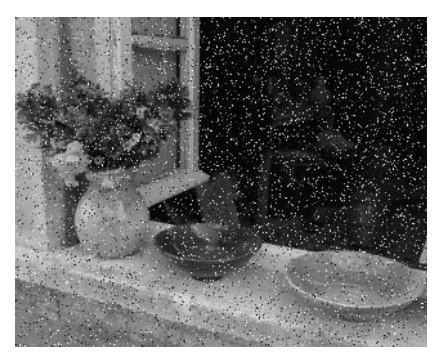
\includegraphics[width=.8\textwidth, height= 5cm, keepaspectratio]{images/filter-example-original-shot-noise.png}}
\caption{Original test image for filter comparison. Shot noise is added on top of the image. Credits \textit{Computer Vision: Algorithms and Applications}~\cite{Szeliski2011}}
\label{fig:filter-example-original}
	\end{center}
\end{figure}

\begin{figure}[t]
	\centering
	\subfigure[Gaussian filtered test image]{
 		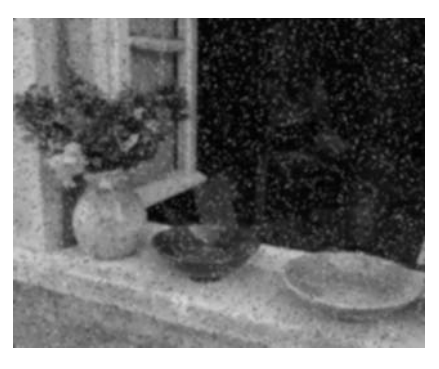
\includegraphics[width=0.4\textwidth, height= 5cm, keepaspectratio]{images/filter-example-gaussian.png}
 		\label{fig:gaussian-filt}
}
	\subfigure[Median filtered test image]{
 		 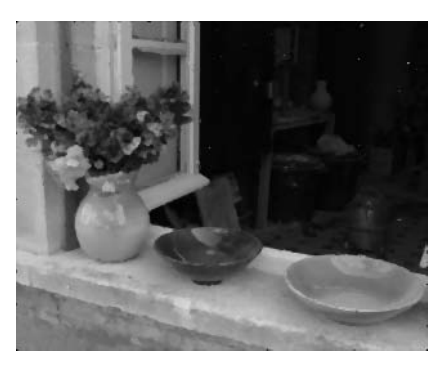
\includegraphics[width=0.4\textwidth, height= 5cm, keepaspectratio]{images/filter-example-median.png}
 		 \label{fig:median-filt}
}
\caption{Test images example taken from \textit{Computer Vision: Algorithms and Applications} \cite{Szeliski2011}}
\label{fig:filter-image-example}
\end{figure}

Figure \ref{fig:filter-example-original} shows a test image where shot noise is added.
Thus, as visible in Figure~\ref{fig:gaussian-filt}, the Gaussian filter, trying to cancel most of the noise, tends to flatten high-frequency details, which are localized close to strong edges.
Contrarily, the median filter, shown in Figure \ref{fig:median-filt}, is more edge preserving.\\
Hence, the median filter was chosen in the initial part of the pipeline of this project for the image pre-processing phase, especially for its capability of preserving the edges, without, then, smoothing away the discontinuities.\\
Bilateral filtering is another type of non-linear operator, which was tested during the development of the designed algorithm.
Basically, during the image pre-processing implementation this specific kernel was one of the analysed options.
As a matter of fact, it is an edge preserving filter as the median kernel.
For this reason, it is one of the most common option for noise cancelling in computer vision algorithm.
Technically speaking, in the bilateral filter, the value of each transformed pixel is a weighted combination of its neighboring pixel values, as defined by the following equality:

\begin{equation}
	\label{eqn:bilateral-filter}
	g(i, j) = \frac{\sum_{k,l} f(k,l)w(i,j,k,l)}{\sum_{k,l}w(i,j,k,l)}
\end{equation}

where the coefficient $w(i,j,k,l)$ is correlated to the multiplication between a \textit{domain kernel}, defined in equation~\ref{eqn:domain-kernel}, and a data-based \textit{range kernel}, illustrate by equation~\ref{eqn:range-kernel}.

\begin{equation}
	\label{eqn:domain-kernel}
	d(i,j,k,l) = \exp \Big( - \frac{(i - k)^2 + (j - l)^2}{2 \sigma^2_d} \Big)
\end{equation}

\begin{equation}
	\label{eqn:range-kernel}
	r(i,j,k,l) = \exp \Big( - \frac{\Vert f(i,j) - f(k,l) \Vert^2}{2 \sigma^2_r} \Big)
\end{equation}

Therefore, the \textit{bilateral weight function} can be finally expressed as:

\begin{equation}
	\label{eqn:bilateral-weight-fnct}
	w(i,j,k,l) = \exp \Big( - \frac{(i - k)^2 + (j - l)^2}{2 \sigma^2_d}  - \frac{\Vert f(i,j) - f(k,l) \Vert^2}{2 \sigma^2_r}\Big)
\end{equation}

However, an unavoidable drawback of the bilateral filter is closely correlated to its computational time, if compared to regular separable filter.
For this reason, as outlined in \cite{Szeliski2011}, multiple acceleration methods have been developed during the last decade.
Nonetheless, those algorithms are prone to a higher memory used w.r.t. the regular filtering, thus they should not be applied to full-color image filtering.\\
A last family of non-linear operators that should be introduce in this section consists of morphological filters.
Regarding the designed algorithm, morphological operators have been actually implemented in the post-processing phase in order to remove small estimation error in the 3D point cloud, enhancing the final dense depth 3D reconstruction of the scene.\\
From a theoretical point of view, \textit{morphological operations} are typically implemented over binary or thresholded images. 
This kind of filtering techniques are executed by first convolving the input image with a binary structuring element, which could have different shapes, and after that the result value is defined basing on the outcome of the convolution.\\
If a binary image $f$ is considered and $m$ is the morphological kernel, the convolution operation is defined as:

\begin{equation}
	\label{eqn:morph-convol}
	s = f \otimes m
\end{equation}

where $s$ is the number of 1s inside each structuring element when shifting through the image.
Therefore, designating $L$, the kernel size, the principal morphological operations, which has been tested in the post-processing phase of the algorithm pipeline, comprise:
\begin{itemize}
	\item \textbf{dilation: } $\mathit{dilate}(f,m) = \theta(s, 0)$
	\item \textbf{erosion: } $\mathit{erode}(f,m) = \theta(s, L)$
	\item \textbf{opening: } $\mathit{open}(f,m) = \mathit{dilate}(\mathit{erode}(f, m), m)$
	\item \textbf{closing: } $\mathit{close}(f,sm) = \mathit{erode}(\mathit{dilate}(f, m), m)$
\end{itemize}

\section{Edge detection and segmentation algorithms}
\label{section:edge-detect-and-segment}

Strictly correlated to the latter family of non-linear operation analysed and to the overall performance of the designed algorithm there is the concept of edge detection.\\
Techniques for finding object boundaries in an image are extremely relevant in computer vision and especially when dealing with stereo matching and disparity estimation. 
As a matter of fact, object borders coincide with occlusion points in 3D, where the majority of wrong matches takes place (in depth estimation). 
Moreover, segmentation methods are strongly related to this topic and remarkably useful in the preparatory phase of an accurate stereo matching algorithm.\\
Specifically to this work, segmentation techniques have not been completely developed.
This was due to the fact that the initial data provided by the laser points grid gives already a good amount of information for obtaining an accurate 3D dense disparity map.
Beside that, after the evaluation of the first reasonable results, further improvements of the algorithm has been considered for enhancing smoothness and continuity among the estimations.
Thus, edge detection and segmentation methods appear to be effective initial operations for multiple reasons, such as, reducing the computational time of the entire pipeline and increasing accuracy and density of the final estimations.\\
Therefore, it is worth to present a brief but exhaustive theoretical outline of the most common edge detection algorithms designed in the computer vision area, considering that they will be part of the future improvements, which will be applied to the work developed so far. \\
From a qualitative point of view edges are usually located in areas where there are changing in color or texture.
However, segmenting an image basing on this information is usually complicated and specific methods has been developed for that.\\
Therefore, for pure edge detection, regions of fast intensity variation are taken into account.
Specifically, edges are usually located in an image where there are steep slopes, in terms of intensity.
Mathematically, these surface's characteristics can be defined through its gradient, i.e.:

\begin{equation}
	\label{eqn:gradient}
	\mathbf{J}(\mathbf{x}) = \nabla I(\mathbf{x}) = \Big( \frac{\partial I}{\partial x} , \frac{\partial I}{\partial y} \Big) (\mathbf{x})
\end{equation} 

where the local gradient vector $\mathbf{J}$ symbolizes the direction of the steepest ascent in terms of intensity. 
Because the percentage of noise is higher at high frequencies, and considering that derivatives enhance those frequencies, a low-pass filter, e.g. Gaussian, is usually applied before the gradient.\\
Nevertheless, to make edge detection really efficient, it would be desired to refine that continuous gradient to the single pixel locations on the edge contours. 
This can be achieved by finding the \textit{local maxima} in the gradient magnitude along its direction.
Therefore, the maxima are calculated by taking the derivative of the gradient, that means apply a dot between a gradient operator and the previous result.
This will lead to the so called \textit{Laplacian}:

\begin{equation}
	\label{eqn:laplacian}
	L_{\sigma}(\mathbf{x}) = \nabla \cdot \mathbf{J}_{\sigma}(\mathbf{x}) = [\nabla^2 G_{\sigma}](\mathbf{x}) \ast I(\mathbf{x})
\end{equation}

where $\sigma$ symbolizes the Gaussian filter used for the initial image smoothing.
This final result is usually called \textit{Laplacian of Gaussian}(LoG) kernel, which is a separable filter.
However, commonly a slightly different kernel is employed, the \textit{Difference of Gaussian} (DoG), which gives a similar result.\\
Hence, once the function $L(\mathbf{x})$ has been defined, its \textit{zero crossing} is computed and so the edge elements can be estimated. \\
Obviously, if high accuracy is needed, higher-order steerable filters can be exploited.\\
Furthermore, taking into account the standard DoG kernel, the fundamental parameter is $\sigma$, i.e. the filter spatial scale parameters.
In fact, it influences the amount of noise on the image and thus the edges scale. \\
It has already been presented that defining confined edges is convenient for multiple applications, such as in the pre-processing image phase of a stereo matching algorithm.
Considering that, combining together these edges, designing a sort of continuous contour, would be even more useful.\\
For example, if the procedure explained above for defining the edges is taken into account, meaning that the edges were defined through zero crossing, link them together becomes quite simple. 
As a matter of fact, adjacent edges have the same endpoints. 
Then, multiple methods exist to encode the edges together forming the contours.\\
Strongly related to edge detections, there is the topic of segmentation, i.e. group together pixels that share the same characteristic.
In computer vision segmentation algorithms are among the first studied and designed topics (\cite{ohlander1978picture}, \cite{Brice1970}, \cite{haralick1985image}) and they are still nowadays a widely analysed problem (\cite{comaniciu2002mean}, \cite{cremers2007review}). 
Some basic segmentation techniques related to the morphological filters has already been presented in the Section~\ref{subsection:neighbor-operator}. 
In this section, the analysis of some commonly used algorithm is carried out.
Since in this field the researches have been numerous simple explanations of some of them, such as \textit{active contours}, \textit{region splitting and merging}, \textit{mean shift}, \textit{normalized cuts} and \textit{binary Markov random fields} are presented. \\
Since the merely theoretical purpose of this analysis and considering that these specific methods have not been widely tested in this project, it is not necessary to describe in detail all of these algorithms.
Therefore, if there would be interest in the mathematical background of the aforementioned techniques, we remind to the manual by Szeliski \cite{Szeliski2011}.\\

\paragraph*{Active Contours}

Active contours \cite{balke1998active} method groups together different techniques, such as \textit{snakes} \cite{kass1988snakes}, \textit{intelligent scissors} \cite{mortensen1995intelligent} and \textit{level set} algorithms.
These methods reach the final solution iteratively thanks to the combination of image and arbitrary user-guidance.

\paragraph*{Region splitting and merging}

Differently from algorithms entirely based on threshold selection and connected components computation, a useful segmentation technique is related to a recursive splitting of the entire image into subregions, which are then merged together hierarchically. 
Therefore, region splitting and merging is fundamentally focused on multiple stages of split and merge of image areas, at different level of density, mainly basing on region statistics. \\
An example of this approach is the \textit{watershed} algorithm \cite{vincent1991watersheds}.
The core of this algorithm stands on dividing the whole image into different \textit{catchment basins}, which are identified taking into account all the local minima present and labelling them. 
In order to make the algorithm suitable also for color images, it is usually applied to the gradient magnitude of the figure. \\
Moreover, an interesting algorithm, which appeared to be useful as a pre-processing phase of more complex algorithms such as stereo matching, optic flow and object recognition, is centred in region merging.
Actually, areas of the image close among each other are combined together considering their average color difference. 
Therefore, if it is below a certain threshold the adjacent portions of the image are merged into a so-called \textit{superpixel} \cite{mori2004recovering}.

\paragraph*{Mean shift}

Mean-shift algorithms, as well as mode finding, k-means and mixture of Gaussian, consider position, color or other features of image points and cluster them as they would be taken from a probability density function, finding the peaks of that distribution.\\

\paragraph*{Normalized Cuts}

The idea of the Shi and Maki algorithm~\cite{shi2000normalized} is to divide the image into groups distinguished by weak affinities, i.e. similarities. 
Therefore, in this methods pixels that show strong similarities will belong to the same group. 
The different groups are, then, separated taking into account the sum of the weights of all the cuts among pixels of different regions.
Because, this could lead to unreasonable clusters, the normalized cut measure is used.


\paragraph*{Markov Random Field}

Markov Random Field (MRF) optimization is an energy-based algorithm.
These energy minimization problems based on MRF are usually solved employing graph cuts techniques.



%\section{Data and estimations error types}
%\label{section:error-types}














%
\chapter{Environment}
\label{chapter:environment}

The developed thesis project is based on a major environment that comprises multiple structures.
First of all, the Middlebury 2014~\cite{Scharstein2014} dataset, which contains detailed stereo pairs, was exploited to perform multiple tests.
Moreover, real indoor rectified stereo images taken with the device designed by the company were employed.\\
In this chapter a brief explanation of the LaDiMo stereo device follows.
Furthermore, it is worth to describe the main characteristics of the dataset adopted.
As a matter of fact, it results extremely useful during the overall designing of the implementation, obtain visual outcomes of the improvements provided to the code.
The ground truth images available in the dataset were especially effective for simulating the behaviour of the company device during the first part of the code implementation.

\section{Middlebury Dataset}
\label{section:middle-dataset}

\begin{figure}[t]
	\centering
	\subfigure[Left Stereo Image Example]{
 		\includegraphics[width=0.4\textwidth, height= 5cm, keepaspectratio]{images/im0.png}
}
	\subfigure[Disparity Left Image Exaple]{
 		 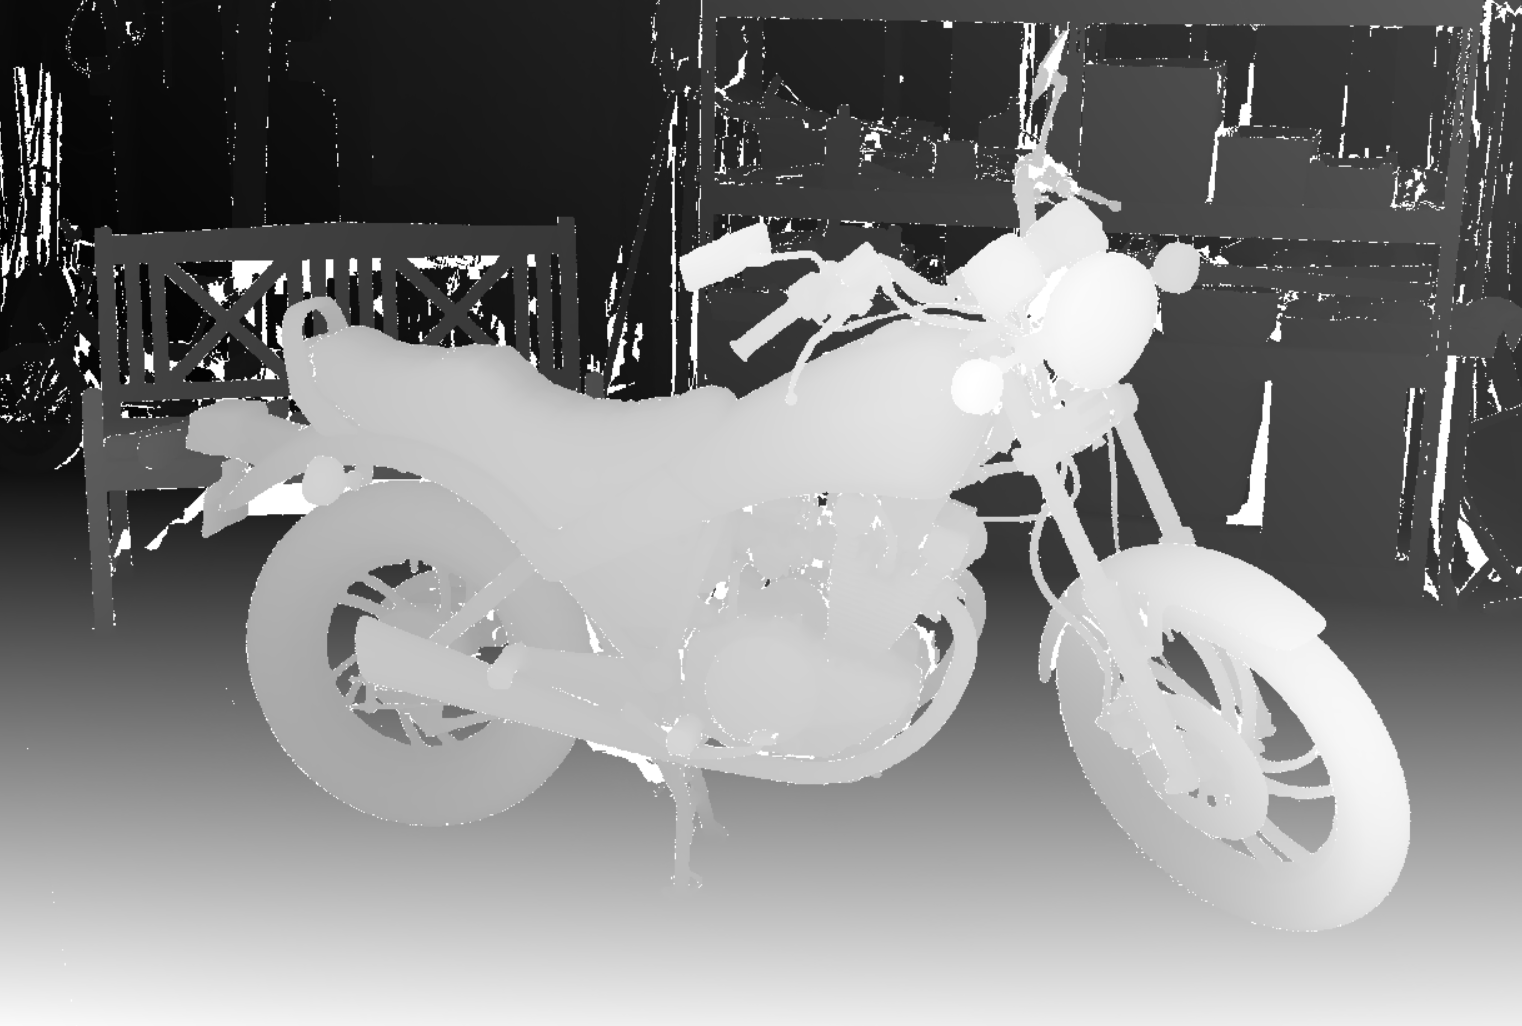
\includegraphics[width=0.4\textwidth, height= 5cm, keepaspectratio]{images/im-0-disp.png}
}
\caption{Middlebury 2014 dataset example}
\label{fig:dataset-example}
\end{figure}

The so called Middlebury 2014 dataset is a high-resolution stereo dataset comprising static indoor scenes and including highly detailed ground-truth disparities.
The images were acquired exploiting a novel structured light system.
This also consists of updated methods for accurate 2D subpixel correspondence search and self-calibration of cameras and projectors with modelling of lens distortion.\\
Generally speaking, Scharstein et al.~\cite{Scharstein2014} provide 33 new indoor 6-megapixel datasets using their system. 
Thus, achieving an accuracy in the disparity estimation of 0.2 pixels on most analysed surfaces, they produce demanding challenges for the stereo algorithms developed since that.\\
That was, in fact, one of their main objective, being the datasets available until their work insufficient in terms of ground truth accuracy, resolution, complexity and realism. 
Therefore, aiming at updating and improving the work of Scharstein and Szeliski~\cite{scharstein2003high}, they obtained Middlebury 2014 dataset, which brought major improvements in the level of calibration accuracy for stereo images.\\
Specifically, the system described in \cite{Scharstein2014} comprises the following novel features: 
\begin{itemize}
	\item a stereo equipment made of two digital single-lens reflex (DSLR) cameras and two point-and-shoot cameras;
	\item a method for robust interpolation of lighting codes and 2D subpixel correspondence search for obtaining accurate floating-point disparities;
	\item bundle adjustment for calibration and rectification procedures;
	\item a robust model selection for self-calibration of structured light projectors and lens distortion;
	\item a so called \textit{imperfect} version of the dataset showing realistic rectification errors.
\end{itemize}  
Figure~\ref{fig:dataset-example} shows an examples of the datasets provided, which comprise the input images, with different levels of exposure, and \textit{perfect} and \textit{imperfect} rectified images with accurate 1D and 2D floating-point disparities, respectively. \\
In order to obtain accurate high-resolution stereo datasets, the authors of the described work based their idea on establishing ground-truth disparities from the input views.
In this manner, calibration problem are prevented and the process can be performed via structured light.
However, the drawback of this is that correct disparities can be achieved only for scene points that are non-occluded in both images.
Therefore, extending the idea in~\cite{scharstein2003high}, that is based on a self-calibration of structured light sources from initial non-occluded disparities, they managed to register illumination disparities in half-occluded regions and model projector lens distortion as well. 
Moreover, imposing initial correspondences they enhance significantly the rectification accuracy.
Then, subpixel precision was obtained exploiting a high number of binary patterns under multiple exposures and applying a robust interpolation.\\

\begin{figure}[t]
	\begin{center}
		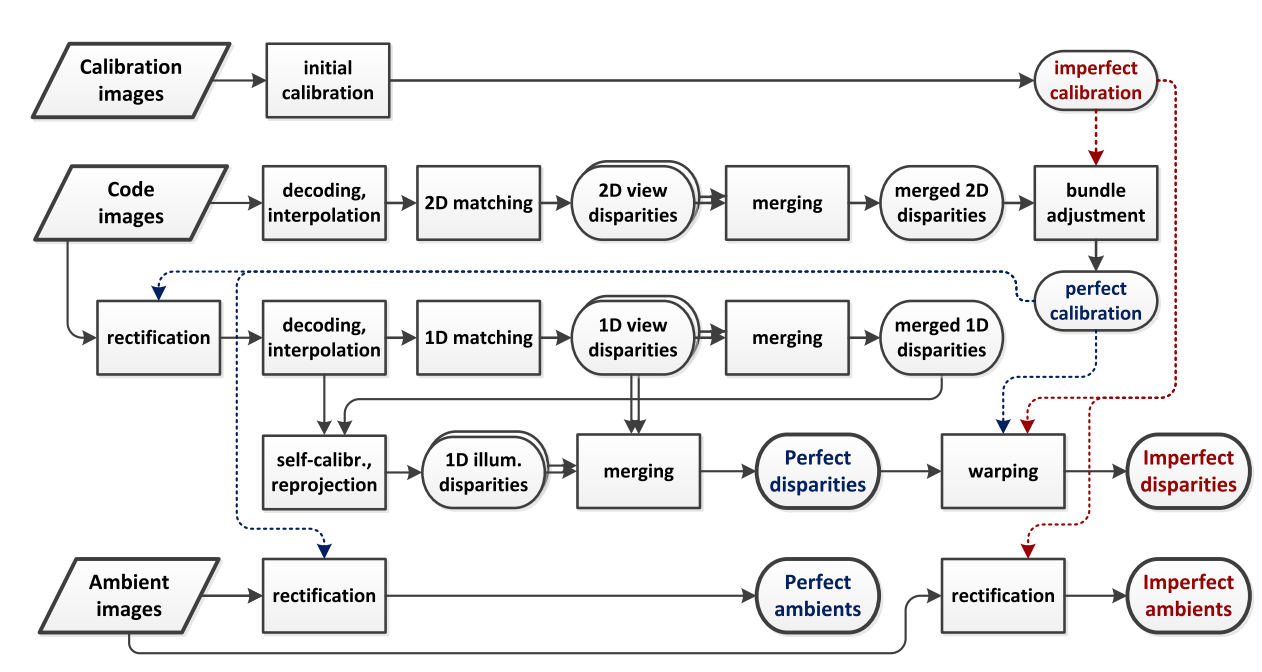
\includegraphics[width=.8\textwidth, height=5cm, keepaspectratio]{images/middlebury-2014-pipeline.png}
		\caption{Pipeline of the overall system for creating the Middlebury 2014 dataset \cite{Scharstein2014}}
		\label{fig:middlebury-pipeline}
	\end{center}
\end{figure}

A brief overview of the pipeline of the process, deeply illustrated in \cite{Scharstein2014}, is now presented.\\
Figure \ref{fig:middlebury-pipeline} depicts the overall pipeline of the system defined by Scharstein et al. \cite{Scharstein2014} for reconstruct the stereo datasets.\\
As simply described, the system's inputs are: calibration images of a standard checker-board calibration target; code images obtained with structured lighting projectors from different positions; \textit{ambient} images collected with multiple lighting conditions. 
First of all, re-factoring operations are applied to the unrectified code images, i.e. thresholding, decoding and interpolation.
This leads to floating-point coordinates of the projector pixel illuminating the scene. 
Thus, the achieved values are employed as unique identifiers to impose the correspondences between the two input images. 
So that, the resulting \textit{2D view disparities} are used to refine the \textit{imperfect} calibration in the bundle-adjustment phase.
The next step of the process is using the rectified input images to generate the \textit{1D view disparity}.
The self-calibration of the projector is, therefore, accessed using the merged disparities and thereby produce the \textit{1D illumination disparities}.
View and illumination disparities are, then, combined together into the \textit{perfect} disparities. 
Last row in Figure~\ref{fig:middlebury-pipeline} shows that rectifying with both calibration allows to achieve the corresponding sets of ambient images.\\
Further details of the single steps of the process are reminded to the original paper~\cite{Scharstein2014} so as not to make the discussion much convoluted.\\
Nevertheless, it is worth to disclose that considering the evaluation of the datasets showed in~\cite{Scharstein2014}, the choice of the Middlebury 2014 images for the initial tests can be assumed as a correct decision.
As a matter of fact, experimental results reported in the original paper demonstrate how that datasets can be considered highly challenging in terms of accuracy and scene complexity.
Therefore, they can be assumed as a useful starting point for recovering information from the ground truth images available and for the stereo algorithm evaluation.\\
As a matter of fact, in the area of dense stereo matching methods, in addition to the Mddlebury 2014, other datasets are available, such as the KITTI 2012~\cite{geiger2013vision} and the KITTI 2015~\cite{menze2015object}, which are among the most commonly employed.
However, as for the authors of~\cite{Keselman2017}, who developed a similar project, the Middlebury dataset was the preferred choice for the tests accomplished during the algorithm designing.
This choice was mainly driven by the high resolution of the dataset, which provides also a desirable subpixel accuracy for the disparity values in the ground truth images. 
In fact, the KITTI dataset, being generated through a LiDAR assisted device, shows less accurate disparity annotation compared to the Middlebury data, especially in occluded areas.

\section{Stereo Photogrammetry LaDiMo device}
\label{section:stereo-device}

\begin{figure}[t]
	\begin{center}
		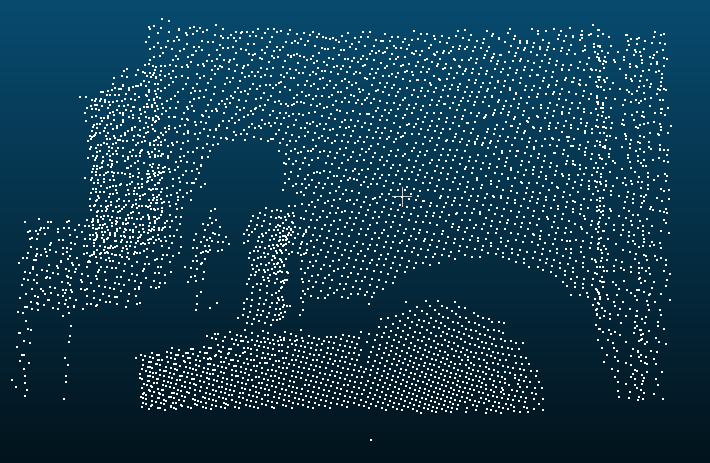
\includegraphics[width=.8\textwidth, height=5cm, keepaspectratio]{images/point-cloud-example.png}
		\caption{Point cloud generated from a test scene}
		\label{fig:point-cloud-input}
	\end{center}
\end{figure}

\begin{figure}[t]
	\begin{center}
		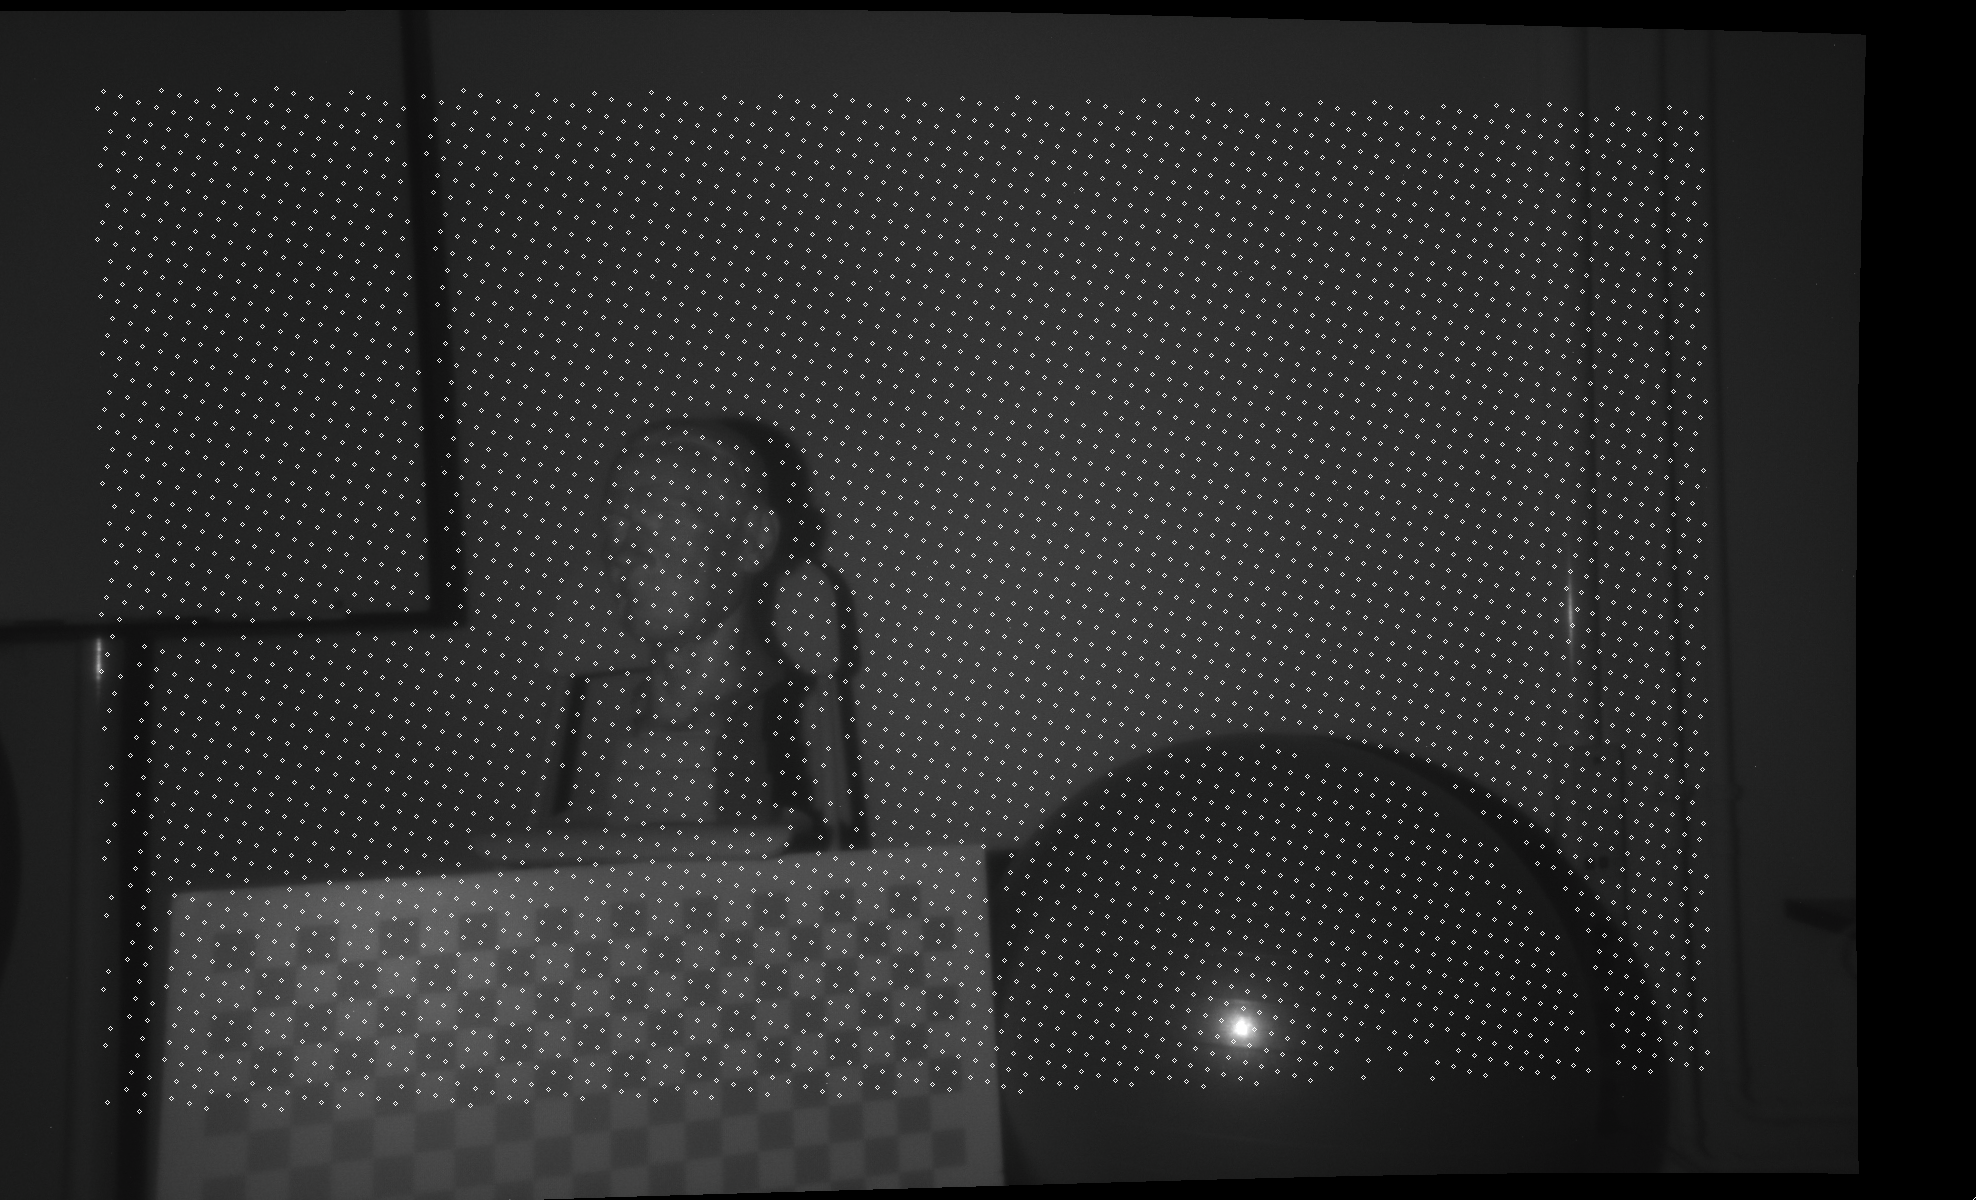
\includegraphics[width=.8\textwidth, height=5cm, keepaspectratio]{images/stereo-rectified-rgb.png}
		\caption{Primary stereo image with Ladimo grid point overlapped}
		\label{fig:primary-stereo-input}
	\end{center}
\end{figure}

\begin{figure}[t]
	\begin{center}
		
\includegraphics[width=.8\textwidth, height=5cm, keepaspectratio]{images/detail-missing-data.png}
		\caption{Detail of the right hand side of the image, close to the ball, where there is a high percentage of missing data}
		\label{fig:detail-missing-data}
	\end{center}
\end{figure}

One of the fundamental mainstay of this Master's Thesis project is the device developed by LaDiMo, the company at which this project has been realized.
Therefore, it is rather useful for a solid understanding of the work done for this thesis to describe, even briefly, the hardware designed by the company and its implementation in the developed work. \\
LaDiMo device comprises multiple structured light assisted cameras. 
Its core functionality is to output a 3D point cloud data of the analysed scene for the listening client. 
Technically speaking, the beams are generated by a laser projector, a collimator lens and a diffractive optical element (DOE), which splits the beams in multiple directions over the scene.
That set of laser points is then accurately measured by a pair of infra-red cameras sensitive to laser's wavelength, which is specifically of $808 nm$.
Moreover, two RGB cameras are additionally mounted on the device, so that sets of stereo images of the scene can be retrieved.
Therefore, this system allows the user to generate a sparse grid of regularly separated points, which contain information on their 3D location, as visualized in Figure~\ref{fig:point-cloud-input}. \\
So that, the described device can be exploited in order to improve in both accuracy and efficiency a stereo matching problem.
This is, indeed, the base of the study presented in this Master's thesis. 
In fact, as already deeply described in Chapter~\ref{chapter:background}, one of the main drawbacks of creating a 3D dense point cloud using stereo matching techniques stands in the aggregation cost part. 
That is, in fact, closely related to the overall range of disparities associated to each stereo pair. 
Moreover, other key factors are the definition of the image size, the amount of texture-less region contained in the analysed scene and the number of edges, which make the algorithms used in those processes even more complicated and computationally expensive. 
However, as visible in Figure~\ref{fig:point-cloud-input} and~\ref{fig:primary-stereo-input}, the laser grid generated with the LaDiMo system cannot be considered enough dense to constitute an accurate 3D representation of the space. 
As a matter of fact, the points hit only some areas of the object and their sparsification does not allow to determine a continuous and smooth change between the surfaces of different objects, or even between different regions in the same object.
Furthermore, as extremely visible in the lower right-hand side of Figure~\ref{fig:primary-stereo-input} and as highlighted in the detail of Figure~\ref{fig:detail-missing-data}, there are sections of the objects that almost completely lacks of points, usually in close proximity of occluded or shaded regions.\\
Therefore, an efficient strategy that can be applied to tackle the problem of creating a dense depth image from a pair of rectified stereo images is to exploit the initial piece of information contained in the grid points data, in order to make the whole process extremely faster, while keeping a high accuracy of the final data.
As a matter of fact, those data can be employed to make the overall pipeline of the algorithm more efficient. \\
First of all, the error rate regarding wrong matches can be highly reduced, then, the disparity range over which the corresponding points are matched can be recursively selected basing on the disparity values of the neighborhood of the analysed point. 
So that, these are only some of the improvement that can be applied to the process utilizing the information that comes from the LaDiMo device.
Thus, as can be therefore understood, the company's system was fundamental for the efficiency of the overall pipeline of the algorithm.
The different steps of the algorithm and the achieved results will be deeply and precisely presented in the following chapters. 
As regards the current analysis of the work, it would be sufficient to introduce the general strategy applied and the reasons that lead to the thought strategy.\\
Taking into account the output of the stereo device, it comprises the two stereo images of the scene, which have to be rectified in order to have the corresponding points along the same scanline for both images, and the grid of points generated from the laser projector and captured by the infra-red cameras, on whose lenses a filter sensible to the laser wavelength is mounted.
Regarding the laser grid, as can be understood from the brief system description, it can be correctly recovered for one of the images only. 
As a matter of fact, the grid points are thus overlapped with the primary image, usually the left one. 
This configuration is, thus, exploited to run the entire pipeline. 
Moreover, it would be also possible to define the corresponding grid for the right image, employing the camera matrix parameters. 
So that, a second reciprocal pipeline could be carried out in parallel. 
In this manner, two different dense depth map are obtained and then handled to apply specific post-processing procedures such as left-right consistency check, which allow to determine possible wrong matches and especially depth values for occluded pixels. 
As aforementioned, the corresponding coordinates of the points can be recovered exploiting the camera matrix parameters, which allow to build up a second grid over the support image. 
However, this phase is not completely necessary for the main purpose of the designed stereo matching algorithm.
It will allow to perform specific post-processing procedures. 
Nevertheless, this has to be evaluated in terms of desired accuracy and computational time, considering that, even simpler post-processing techniques, such as morphological, bilateral and median filters has shown to give an accurate 3D dense point cloud.

\section{Software Environment}
\label{section:software-env}

Considering the programming related part of the built environment, it comprises multiple software and platforms. 
Although, some computing environments and frameworks were not entirely employed during the overall designing of the project.
This was due to the way in which the work was conceived and the choices regarding the applicable strategy. \\
As a matter of fact, in the initial phase different methods and approaches have been tested using MATLAB\footnote{The software was used for academic purposes being available through the personal university account}. 
Despite the known fact that further working implementation of the algorithm would not be run using an academic version of the aforementioned software, only a first researching phase was initially planned.
Multiple reasons support that decision, such as a personal considerable knowledge of the software and its built-in libraries and functions, the possibility to check the results of the performed tests in an user-friendly manner and the side own need to get confidence with the company's hardware and software environment.\\
Taking those aspects into account, the initial part of the work was dedicated to research and tests necessary to evaluate the proper strategy for the algorithm development and to conduct comparisons between some initial ideas over different available methods.

\subsection{MATLAB computing environment}
\label{subsection:matlab-env}
As introduced above, primary tests have been handled using MATLAB\textsuperscript{\textregistered} and especially some built-in functions correlated to stereo matching and image manipulation.\\
MATLAB can be defined as a platform composed of a multi-paradigm\footnote{functional, imperative, procedural, object-oriented, array} numerical computing environment and a proprietary programming language created by MathWorks.
It is significantly used for matrix manipulation, algorithm implementation and plotting of data and functions.
Moreover, one of its most utilized packages is Simulink, which allows the user to develop even extremely complex algorithms, especially for dynamic and embedded systems, with a block-based interface. \\
Although its high versatility and possibility to design programs that can be run of different systems, it was decided not to make it the main environment of the project, in order to not be limited from both software and patent perspectives.\\
Consequently, after the initial preparatory phase of the project, the primary development of the algorithm has been realized through a C++ code, which has been built up using Microsoft Visual Studio and the OpenCV library. 

\subsection{Microsoft Visual Studio integrated development environment}
\label{subsection:visual-studio-env}

Microsoft Visual Studio is an integrated development environment (IDE) crated by Microsoft. 
It is used for several purposes, such as software development, websites, web services, mobile as well as web applications. 
Obviously, it is based on Microsoft software development platforms, e.g. Windows API, Windows Form and Windows Presentation Foundation. 
It is also advisable to mention some of its assets, which make it the most preferred IDE, in terms of popularity\footnote{According to data from Google Trends and available at \url{https://pypl.github.io/IDE.html}}. \\
First of all, it allows to create both native, or machine language, code and managed code.
Moreover, among its most powerful features there are IntelliSense, the intelligent code completion included in the editor, and the integrated debugger, which operates both as source-level debugger and a machine-level debugger. 
Furthermore, it contains lot of other built-in tools, designed for multiple applications and objectives, plug-ins that enhance coding capabilities and it supports almost any programming language.\\
Considering specifically its architecture, it actually does not support inherently any programming language, solution or tool.
Rather, it permits the integration of functionalities coded as VSPackage, i.e. Visual Studio Package, which are software modules that broaden the Visual Studio IDE by supplying UI elements, services, projects, editors and designers. 
Therefore, at its native behaviour, it works as a \textit{Service} solution. 
As an example, the support for programming language is added by using a specific VSPackage knows as \textit{Language Service}.
Exploiting that service various functionalities can be included in the IDE. 

\subsection{C++ programming language}
\label{subsection:c++-env}

Subsequently to the initial preparatory phase, in which the main employed environment was MATLAB, the actual design of the final algorithm has been developed basing on the C++ syntax.\\
The decision of exploiting MATLAB only for the initial planning of the work and for the first tests correlated to the feasibility of the various ideas was mainly due to multiple reasons, which cover different aspects of the entire design of the project.
First of all, since the beginning there was the intention of designing an algorithm that would be adaptable to different types of hardware and which would be further adjusted to other programming languages, e.g. CUDA, in order to obtain better final performances.
Moreover, considering plausible forthcoming commercial issues, there was the need to ensure a developing as free from copyright as possible. 
Flexibility and efficiency were other fundamental drivers of that choice. 
As widely know in the technological field, C++ programming language can ensure velocity and efficiency of the designed software as well as flexibility with different types of hardware.
In fact, it can be optimal for coding both at high levels of abstraction, and at low levels, e.g. at machine language level.
Then, in relation with this very project implementation, using C++ was possible to widely exploit the functions of the OpenCV library. \\
Therefore, adopting C++ as the fundamental programming language of this Master's Thesis project, it was possible to reach a sufficient level of computational speed, trying to minimize the memory requirements and simultaneously keep a high amount of abstraction, necessary for working effectively in the computer vision field. 

\subsection{OpenCV cross-platform library}
\label{subsection:opencv-env}

OpenCV, Open Source Computer Vision Library, is a library of programming algorithms primarily intended at real-time computer vision.\\
It was employed as a fundamental support structure of this project mainly because of the functions accessible in that library, the fact that it is open source and the remarkable documentation available. 
Moreover, thanks to those algorithms, the implementation of methods and functions inside the project pipeline became faster, more reliable and multiple pre-processing and post-processing techniques has been tested, following structural changing in the main algorithm structure.\\
Therefore, OpenCV library can be considered as an important resource of this work.
For that, and for more theoretical purposes, it is appropriate to introduce the main features of that computer vision based library.\\
First of all, OpenCV was initially developed by Intel, then later maintained by Willow Garage, a robotic research lab and technology incubator and subsequently by Itseez, currently acquired by Intel.
Precisely, the library is cross-platform and open-source, under BSD, Berkeley Software Distribution, license. 
The library was initially created to advance CPU-intensive applications, related to real-time tracing and 3D display walls project.
Considering that, it is therefore clear why it is widely exploited when dealing with computer vision correlated works.\\
As defined in~\cite{bradski2008learning}, the main targets of the initial project were:
\begin{itemize}
	\item Accelerate vision research providing open and optimized code for essential vision framework.
	\item Aim for a more readable and interchangeable code by providing a universal infrastructure to use.
	\item Enhance vision-based commercial projects by producing a portable and optimized code available with a free license.
\end{itemize}
Currently, OpenCV library is one of the most used platform by computer software companies.
As a matter of fact, it has been calculated that it counts more than 47 thousand people of user community and an evaluated number of downloads surpassing 18 million \footnote{Data from \url{https://opencv.org/about/}}.\\
Thus, it has been chosen as one of the main assets of the developed work, because of the aforementioned reasons, and in relation to the available applications, which can be used in multiple computer vision related areas, such as, 2D and 3D feature toolkits, facial recognition systems, mobile robotics, object detection, segmentation and recognition and diverse machine learning fields.


\subsection{CloudCompare 3D editing and processing software}
\label{subsection:cloud-compare-env}

CloudCompare is a software that was exploited during this project almost exclusively for the accurate 3D point cloud visualization, which it can easily provide.
Therefore, it can be considered as a side software used in this work, which helps to get coherent visualizations of the result, things that results difficult or overcomplicated employing OpenCV functions and C++. 
On the contrary, with this software was easy to visualize the computed results, and deeply understand if the modifications made in the code work correctly, improving the final result.\\
Therefore, to provide a brief presentation of this software, it is basically a 3D point cloud processing software.
Originally, it was developed to operate comparisons between two dense 3D points clouds, such as the ones collected with laser scanner, or between a point cloud and a triangular mesh.
On top of that, it has been further expanded to a more multi-purposes point cloud processing software, providing multiple advanced algorithms for data handling and processing. 

%
\chapter{Methods}
\label{chapter:methods}

A properly planned project requires the analysis of multiple methods and strategies that can be applied during its design. 
Therefore, this chapter displays, focusing on the multiple aspects of the entire project, the different techniques, encountered revising the broad literature accessible in this field, and the decisions that brought to the actual development of the algorithm, which will be thoroughly described in the chapter \ref{chapter:implementation}.\\
In this chapter, an extensive outline of the work made is not produced, though. 
Instead, the following sections focus on a concise, but anyway exhaustive, tracing of the methods available for a correct dense disparity estimation and for image data processing.
Concurrently, the choices made for the specific aspect of the algorithm are defined and explained.

\section{Standard disparity estimation methods}
\label{section:std-methods}

An extensive and broad analysis of the standard and the deep learning methods for dense disparity estimation has already been presented in chapter \ref{chapter:background}, where the review of the literature related to this Master's thesis project has been carried out.
Nevertheless, these sections focus on a different aspect of that analysis, which is correlated to the algorithms that turned out to be the most relevant for this work and to the features of some of the current machine learning based techniques, which appear to be applicable to this project.\\
Considering the standard algorithms for recovering a dense depth image from a stereo pair, the initial approach on which it was decided to focus on for the designing of the project refers to the Semi-Global Matching (SGM) stereo method developed by Hirschm\"{u}ller \cite{Hirschmuller2008}.
The decision of starting to concentrate on that evaluation of the stereo matching problem was mainly driven by the recent methods designed for dense disparity estimation.
As a matter of fact, most of the algorithms created in the last decade are based on the Hirschm\"{u}ller idea or, at least, they make reference to several aspects of the functions outlined in \cite{Hirschmuller2008}.
This fact is clearly comprehensible considering that the SGM method was classified as the best algorithm at the time of its publication and it is currently one of the top-ranked algorithm in terms of sub-pixel accuracy and computational time.
Hence, taking into account the benchmark data based on two of the most employed dataset, i.e. Middlebury \cite{Scharstein2014} and KITTI \cite{geiger2013vision} datasets, and after an initial general review of the literature publish in this field, it results that the top-performing algorithms use key features of SGM in their main pipeline. 
Moreover, it is worth to point out that the majority of the most accurate real time deep learning based algorithm tends to adopt the main functions of the SGM model, exploiting neural networks to ensure real time evaluations of the disparities.
Therefore, it was initially though that a reasonable option for the developing of an algorithm, which would work in real time providing accurate outcomes, would focus the attention of the Hirschm\"{u}ller method.\\
As already introduced in section \ref{sec:stereometh}, the SGM method combines the idea of the standard local based algorithms, where the main cost calculations are made over limited size windows, and global algorithm, for which the best pixel disparity estimation is based on a global energy function. 
Thus, mainly because its hierarchical cost calculation, SGM method outperformed the top-ranked algorithm over the dataset \cite{scharstein2003high}, proving real-time performance of that dataset images. 
However, with the current dataset, such as Middlebury 2014 \cite{Scharstein2014}, KITTI 2012 \cite{geiger2013vision} and KITTI 2015 \cite{menze2015object}, the standard Semi-Global Matching algorithm provide optimal results in terms of accuracy but it tends to slightly suffer if computational time is considered.
For this reason, the most recent real time methods for dense disparity estimation establish the cost computation part of their pipeline over the SGM idea, although, they exploit hardware efficiency or even neural network structures to reach extremely fast computations.\\
Thus, considering this project, it was decided to initially build up the main pipeline on the SGM method structure and employ the stereo device designed by the company to reach real time performances, without loosing in accuracy. 
Furthermore, as previously anticipated, an upstream choice was made. 
As a matter of fact, the current top-performing algorithms strongly depend on convolutional and deep neural network to achieve fast computations.
Contrarily to that, we decided to based the skeleton of our method on the data available through the stereo system to reach a real time implementation.
In this manner, all the problem related to the shifting between synthetic and real environment, faced by deep learning algorithms, would be avoided. \\
The first outline of the algorithm was, hence, partially based on the Semi-Global Matching method \cite{Hirschmuller2008}. 
In order to analyse the suitability of the implementation, absolute computational time performances were not initially taken into account. 
At first it was chosen to focus on the relative efficiency that would be estimated among the different methods used in the principal pipeline.\\
As aforementioned in chapter \ref{chapter:environment}, these preliminary evaluations has been developed in MATLAB. 
In that phase an implementation sufficiently similar to the standard SGM method was designed. 
Thus, the focus was centred on the different types of algorithms used for matching the corresponding pixels and, then, on the part of the pipeline related to the matching and the aggregation costs, as precisely defined by Scharstein and Szeliski in \cite{Scharstein2001}.
The adoption of this working strategy was due to the following motivations. 
First of all, the predominant research aim of this project, whose purpose would most likely further shifts in more market based one, then the need of test the effective performance in accuracy of pure SGM based method and the requirement of analyse the relative efficiency between that algorithm and our method, whose pipeline would be based on the information acquired exploiting the company device. \\
Considering that a fundamental part of this initial testing phase was focused on the matching cost evaluation, multiple matching algorithm has been tested in order to find the most efficient one mainly in terms of accuracy. 
Therefore, basing on the work done in \cite{Hirschmuller2007}, \cite{Patil2013} and \cite{Ko2017}, and making reference to the algorithm used for computing visual correspondence described in \cite{Zabih1994} and \cite{Demetz2013}, the performance of different matching cost algorithms has been analysed.\\

\subsection{Census transform}
\label{subsection:census-transform}

A crucial phase of the SGM algorithm stands in the matching cost computation.
As briefly explained in Chapter \ref{chapter:background}, this cost is evaluated by computing the difference in the value of intensity among corresponding pixels.
Therefore, especially when dealing with unexpected luminance variation inside the analysed scene, it comes out that non-parametric local transforms are optimal as the support for that correlation \cite{Zabih1994}.
As a matter of fact, these kind of measurements do not rely on the actual intensity values of the pixels, but on the relative local intensities instead.
Therefore, using this kind of models, a considerable number of outliers can be tolerated and improved results are visible especially along object boundaries.\\
Among the commonly used and best performing non-parametric local transform, census and rank transform are described.
Moreover, couple of different implementations of those two classes of transform are introduced.\\
It is widely known in computer vision field that correspondence problem is crucial in depth estimation from stereo pairs.
Correspondence can be, thus, defined by transforming the images with a specific method and then establishing correlations.
In that, the key factor is the transformation, which must tolerate unexpected variation in intensity, for example due to unwanted light source, and in general changes in image bias and gain.\\
Therefore, non-parametric area-based transform rely on local ordering of intensities and not on the actual intensity values.
If an image is considered, and defining as $p$ a random pixel, its intensity becomes $I(p)$. 
Then, let $N_d(p)$ be the set of pixel in a certain square neighbourhood of size $d$, where $p$ is the central pixel. 
Hence, the binary function $\xi(p, p')$ takes value 1 if $I(p') < I(p)$, 0 otherwise.
A non-parametric local transform only rely on the set of pixels in the specific neighbourhood.
Therefore, the \textit{Census transform}, $R_{\tau}(p)$ maps the image subregion surrounding $p$ to an array of bits representing the set of local pixels whose intensity is less or equal than that of $p$. 
Mathematically, the census transform can be formulated as:
\begin{equation}
	\label{eqn:census-transform}
	R_{\tau}(p) = \bigotimes_{[i, j] \in D} \xi(p, p +[i, j])
\end{equation}
where, $N(p) = p \oplus D$, with $\oplus$ is the Minkowski sum and $D$ the set of displacements, and denoting with $\otimes$ the concatenation. 
After the census transform has been applied, the actual comparison among corresponding pixels in done by computing their \textit{Hamming} distance.\\ 
Higher accuracy in corresponding pixel matching can be achieved using an extension of the Census transform, defined as center-symmetric Census transform \cite{Spangenberg2013}.
Therefore, if a square image subregion is taken into account, which has dimensions $n \times m$, we already know from equation \ref{eqn:census-transform} that $s(u, v) = 0, if u \leq v, 1$ otherwise, where now $s( )$ is the sign function.
Precisely, in this notation the census transform can be thus defined as:
\begin{equation}
	\label{eqn:census-transf-2}
	CT_{m,n}(x, y) = \bigotimes_{i = -n'}^{n'} \bigotimes_{j = -m'}^{m'} s(I(x, y), I(x + i), y + j)
\end{equation}
where $n' = [n/2]$, and $m' = [m/2]$.
Hence, as shown in Figure, the center-symmetric census transform can be mathematically defined as:
\begin{equation}
	\label{eqn:center-symmetric-census}
	CS-CT_{m,n}(x, y) = \bigotimes_{(i, j) \in L} s(I(x - i, y - j), I(x + i, y + j))
\end{equation}
where $L = L_1 \cup L_2$, $L_1 = R_{-n',0} \times R_{-m',0} \setminus {(0, 0)}$, $L_2 = R_{1,n'} \times R_{-m',1}$ and $R_{a, b} = {x \in \mathbb{Z} \vert a \leq x \leq b}$.
Because, only center-symmetric pairs of pixels are compared, the formulation in equation \ref{eqn:center-symmetric-census} needs less bit than the one in \ref{eqn:census-transf-2} to describe the same patch. 
As aforementioned, the actual matching cost is then computed using the Hamming distance between corresponding pixels. 

\subsection{Rank Transform}
\label{subsection:rank-transform}

\begin{figure}[t]
	\centering
	\subfigure[Grayscale pixel intensity values]{
 		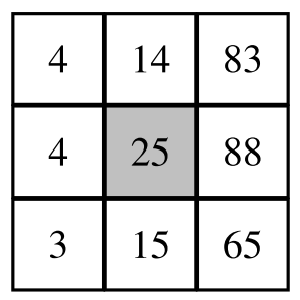
\includegraphics[width=0.3\textwidth, height= 5cm, keepaspectratio]{images/patch-rank-example.png}
}
	\subfigure[Rank transform ]{
 		 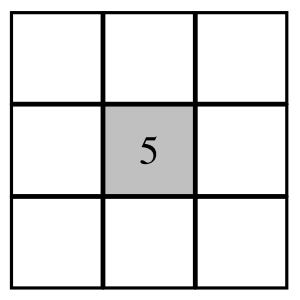
\includegraphics[width=0.3\textwidth, height= 5cm, keepaspectratio]{images/rank-signature.png}
}
\subfigure[Complete Rank transform]{
 		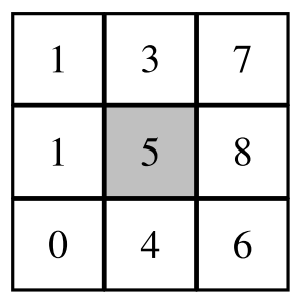
\includegraphics[width=0.3\textwidth, height= 5cm, keepaspectratio]{images/complete-rank-signature.png}
}
\caption{Example patch with grayscale pixel intensity values}
\label{fig:rank-example}
\end{figure}

Another patch-based pixel descriptor is the Rank transform.
As the Census, it is morphologically invariant.
Therefore, it is not sensitive to any monotonically increasing of the grayscale intensity values. \\
The definition of this measure is, actually, quite simple.
The pixels in the specific patch considered are ordered basing on the ranking of all grayscale values in that area. 
Then, the reference pixel \textit{rank encoding} is determined by counting the number of neighboring pixels with a gray value smaller than the considered pixel, that is, basically, its position in the intensity ranking of the patch.
Figure \ref{fig:rank-example} shows a $3 \times 3$ example patch where the central pixel, i.e. the reference one, is map to its scalar rank encode. 
This patch-based descriptor, as the Census transform, was introduced by Zabih and Woodfill \cite{Zabih1994} and, defining an image pixel with $P$ and its neighborhood with $N(P)$, it can be mathematically expressed by the following equality:

\begin{equation}
	\label{eqn:rank-transform}
	R(P) = \Vert {P' \in N(P) \vert I(P') < I(P)} \Vert	
\end{equation}

Looking at the mathematics of the Census and the Rank transforms, it is evident that the former encodes more information. \\
In addition to the two presented non-parametric local transforms, there is another area based descriptor that need to be mentioned.\\
The Complete Rank transform can be thought as an improvement of the Rank transform.
It was more recently presented by Demetz et al. \cite{Demetz2013}, with the goal of keep a higher amount of information with respect to its standard version.
Actually, it works in the following manner.
At first the normal Rank transform is applied to all the elements of the patch. 
Then, these ranks are concatenated, as it is done for the Census, so that the complete rank descriptor is generated.  
As visible in Figure~\ref{fig:rank-example}, pixels with the same intensity take the same rank value. 
Therefore, the encoding for the patch displayed in the image is:
\begin{equation}
	\label{eqn:complete-rank-encoding}
	\mathbf{enc}_{CRT} = (1, 3, 7, 1, 5, 8, 0, 4, 6)^\top
\end{equation}

\subsection{Conventional intensity based methods}
\label{subsection:conventional-methods}

\section{Deep-learning based methods}
\label{section:deep-learning-method}

As introduced in section~\ref{subsec:deeplearnmeth} the deep learning method approach for stereo matching was not chosen as the base method for the developing of this project for different reasons, which have already been explained in Chapter~\ref{chapter:background}.\\
However, the structure of a deep learning based project was extremely useful in the definition of the strategy used for the designing of our work.
Fundamental is the novel stereo matching method developed by Poggi et al.~\cite{Poggi2019}, who exploited a small quantity of sparse initial depth data to enhance the overall stereo matching problem.
In their paper, they presented \textit{Guided Stereo Matching}, an innovative stereo algorithm, which uses a sparse set of accurate depth measurement obtained from reliable hardware system, e.g. a LiDAR, with the aim of improving the general performance of a standard depth estimation algorithm.\\
Therefore, considering the structure of our system, the strategy used in \cite{Poggi2019} appears to have valuable insights, which would be exploited in the definition of our own work.
Actually, they proposed to use sparsify yet reliable depth measurements for the following tasks: improve the general accuracy of the neural network designed for achieving the depth estimations, reduce the domain shift, i.e. the drops in accuracy that deep learning based methods face when dealing with data from a new environment, and the potential improvement of result when training the network starting from that sparse set of inputs.\\
Similarly to that approach, in this project, we decide to base our overall estimations on the knowledge of the sparse group of 3D measurements coming from the company device.
However, differently from them, the algorithm described in this thesis uses as the standard methods in the  stereo matching pipeline, which appear to work better for multiple types of environments. \\
Thus, taking into account the results provided in~\cite{Poggi2019}, where the authors demonstrate how their strategy outperforms the current state-of-the-art stereo matching methods, we assumed that a reasonable approach to apply would exploit the initial cues coming from the laser grid of points in order to improve the performance of the main algorithm. 
As a matter of fact, in their paper, Poggi et al.~\cite{Poggi2019} assert that the initial set of estimations can be obtained with whatever device that can give sparse data.\\
Consequently, during the initial stages of the development some tests have been performed designing a simulated point grid, in order to have a clear outcome of the reliability of this strategy.
Hence, employing the Middlebury 2014 dataset, the initial set of clues was designed taking the sparse depth information from the ground truth images available. 
Obviously, the depth measurements coming from the dataset can be considered highly accurate, differently from the data from the LadiMo device, which would most likely be affected by some sort of noise, mainly Gaussian. 
Nevertheless, it is actually extremely useful to perform these tests in order to figure out since the first phases of the project, the qualitative performance of the adopted strategy.
The details of the conducted tests are widely described in Chapter~\ref{chapter:implementation}, where some of the temporary results obtained are proposed too.\\


\section{Pure derivative based data estimation algorithm}
\label{section:deriv-based-algorithm}

As previously introduced, two different algorithm structures have been implemented and compared in this project, in addition to the standard Semi-Global Block Matching (SGBM) algorithm, whose result was used as a baseline for carrying out an appropriate comparison with the novel implementation designed. 
Therefore, the first one of these methods is closely related to the standard SGM implementation, it exploits the initial knowledge of the sparse depth estimations, however, the core of the algorithm follows the Hirshm\"{u}ller algorithm \cite{Hirschmuller2008}. 
Differently, the other implementation designed is more strictly related to the initial sparse depth clues, and it is focused on those for the overall pipeline of the algorithm.
As it will be reported in Chapter~\ref{chapter:evaluation}, this latter approach will provide a faster yet, in general, equally accurate implementation.
Therefore, these two designed strategies will be deeply explained in Chapter~\ref{chapter:implementation}.
Beside that, it is worth to propose here a concise outline of both of them, in order to introduce their main features.\\
Regarding the last introduced method, it highly exploits the information coming from the input sparse clues.
Therefore, starting from that initial 3D point cloud and using a pair of stereo images of the considered scene, a dense point cloud is built by estimating the space positions of an high amount of scene points. 
The key of this algorithm actually stands on the way in which those estimations are carried out. 
Thus, considering the point grid given by the stereo device, the local derivatives among neighboring points are evaluated. 
These will be then used for two main scopes: identify if inside a specific subpatch of the point cloud there could be an edge, that is that points belonging to the same small cluster have indeed highly different values of depth, and for computing the denser point cloud by interpolating the 3D value of neighboring points and exploiting the values of the pre-calculated derivatives for making the interpolation faster.\\
It can be, hence, easily understood how core of this strategy stands on the local derivatives estimation. 
As a matter of fact, let us consider a square cluster of 4 neighboring points from the initial point cloud, it is possible to evaluate the \textit{internal} and the \textit{external} derivatives among these points.
Specifically, the former are referred to be identified by the vectors that points \textit{inside} the square patch. 
Instead, the external derivatives are said to be the ones evaluated using the other points, which are neighbors to the patch corners. 
Figure \textbf{PUT FIGURE HERE} shows the aforementioned point cloud patch. 
Summarizing, the denser 3D point cloud is estimated by filling up each one of the subpatches that can be identified from the initial grid. 
In order to perform this, the estimations are carried out exploiting the derivative vectors, which are weighted by the distance from the new estimated point and each one of the window corners.
This detail, in fact, shows that four temporary estimations are done for each new point. 
In this way, the best estimation is actually chosen by projecting the evaluated 3D point to the image plane and calculating the matching cost between the corresponding pixels for each temporary estimation.
For the matching cost, as it will be more widely explained in Chapter~\ref{chapter:implementation}, different methods have been investigated.
However, the plain absolute difference appeared to be the best in terms of performance for that algorithm.
In fact, at the end of the whole computation, similar results have been found with different matching cost algorithms.
Hence, in that case, it is worth nothing to use most expensive methods, which will make the computations heavier giving only slightly better results.
Besides that, specific penalties have been added on top of the pure matching cost to enhance the distance from the respective window corner in terms of x and y coordinates.\\
Summing up the general outcome gained from this approach, it results to be a lightweight yet effective method.
As it will be presented in the Chapter~\ref{chapter:evaluation}, this algorithm provides 3D dense point clouds that can be considered sufficiently accurate for a general use employing a relatively low amount of resources.
Despite that, internal parameters of that method can be adjusted, depending on the user needs, in order to obtain outcomes with a different grade of accuracy. 
Evidently, this will affect the performance in terms of computational time and used resources, however, this is always considered for every testing environment. \\

\section{SGM based data estimation algorithm}
\label{section:sgm-based-algorithm}

As aforementioned, the second method that has been designed is based on a more standard approach, closely related to the SGBM algorithm. 
Basically, it exploits the information coming from the input point grid to make the standard pipeline of the SGBM method faster, which could be extremely expensive when dealing with high density images.
Actually, the initial points information is employed to select the disparity levels on which the main algorithm is run. 
Simply speaking, the final implementation can be considered as a \textit{disparity-wise} Semi-Global Block Matching, where there are not usually continuous changing in the disparity levels, especially if edges are detected inside the specific image patch.\\
Taking into account the general performance of this approach, it runs slower than the previous strategy. 
Moreover, the final 3D point cloud shows an higher density, however, looking at the achieved results, the increase in accuracy obtained in this case seems not to be worth it the observed rise in computations. \\
Therefore, at the reached stage of the project, it appears that a slightly decrease in accuracy can be considered reasonable for a quite high increase in computation speed. 
However, every use case has to be widely analysed in order to choose the most profitable solution.
Additionally, it is necessary to point out that this project should be regarded as still in a researching phase. 
Multiple tests have been performed with both dataset, i.e. almost perfect, and real images. 
However, for a good analysis of the specific use case, it is necessary to run various tests on the specific working environment, and eventually, adjusting parameters or side sections of the main pipeline.\\
Beside that, a further discussion over those topics will be presented in Chapter~\ref{chapter:discussion}. 
Anyhow, it was considered helpful for a deeper understanding of the results that will be presented in the Chapter~\ref{chapter:evaluation}, to introduce also here some brief comments over the outlined algorithms.\\
Hereafter, a short overview on the pre and post-processing techniques employed in the whole project is presented. 
Further details will be described in the following chapter. 
Anyway, it is useful to introduce here the main techniques used and especially the differences in performance, which have been analysed, and also their scope in relation to the final accuracy of the algorithms.

\section{Pre-processing techniques}
\label{section:pre-process-tech}

In the first section of the algorithm pre-processing techniques have turned out to be, not indispensable, but useful for the accuracy of the final results.
The focus was especially centred on the noise removal. 
As a matter of fact, if a stereo pair is given, it is generally affected by Gaussian, i.e. random, noise, which can be due to multiple reasons, such as instability of environmental conditions, lightning, local temperature gradients that can affect the stereo system or errors in the setting of the stereo device. \\
Therefore, for those reasons and for the purpose of launching the algorithm having the input image as clearer as possible, especially in terms of pixels' intensity, blurring filters have been tested and analysed during the development of this first phase of the pipeline. 
Specifically, median and bilateral filters occur to be ideal for smoothing away noisy components in the frequency spectrum, keeping the performance of the whole algorithm reasonable. \\
The details of that analysis are left to Chapter~\ref{chapter:implementation}.
However, it is worth to indicate that, even if heavier from a computational side, the median filter came out as the preferred choice for image blurring when dealing with real stereo pairs.
As a matter of fact, when the images from the datasets have been tested, there was not any needs to apply some sort of pre-processing, being them already cleaned from noisy components. \\
Talking about the real dataset and especially about the initial grid of points obtained from the company stereo device, some pre-processing operations have been performed over those data too. 
The goal of this process was the requirement of starting the main computations basing on accurate and possibly complete data. 
Focusing on that, it actually happened that the input point cloud was, in general, not fully complete. 
Instead, some of the points had missing data.
This was probably due to occlusion, in fact most of the \textit{bad} points areas were located on edges or on regions affected by shadows. \\
Therefore, this problem was tackled in the following way.
First of all, all those input data have been analysed and, specifically, the percentage of completely missing values with respected to the total amount of points was calculated. 
This was performed to obtain an initial estimation of the percentage of errors present in the input data, thus to evaluate the degree of effort that it should be required to have a final accurate result.
Precisely, let us think about the case of having an extremely low amount of errors, e.g. the 1.5\% of the entire point cloud. 
Moreover, consider the condition in which these errors are sparsified and, additionally, that would be sufficiently complicated to fill in those missing data.
Thus, in this situation, it would be worth nothing to spend resources to improve the completeness of the input data, reaching an outcome that would be, most likely, only slightly more accurate and for which the whole algorithm would be way heavier and more complicated. 
On the contrary, a feasible option can be the one of running multiple time a very lightweight algorithm, exploiting the most accurate new estimated points to improve the density of the successive 3D clouds.\\
For the actual purposes of this Chapter it is unnecessary to present further details of this data processing, which would be more widely analysed in the following sections. \\
On the other hand, it is convenient to introduce here some features about the post-processing operations, which have been carried out in the last section of the algorithm.\\

\section{Post-processing techniques}
\label{section:post-process-tech}

Considering the results achieved with both the Middlebury 2014 dataset and the real environment images an additional blurring process has been run over the final data. 
Differently from the the smoothing operations employed in the first part of the depth estimation method, in this phase the morphological filters emerge to be the most appropriate trade-off between final result and computational resources. \\
Also during the designing of this area of the project several tests have been carried out in order to obtain an estimation of the most suitable post-processing technique to run over the final result.\\
Therefore, considering the disparity images achieved using the stereo pair from the \textit{perfect} dataset, the application of an additional median filter seemed more appropriate.
However, for the outcome accessed using images taken with the LadiMo device, the use of morphological filters appear more convenient. 
Additionally, several of those have been tested. 
Opening, closing, erosion and dilation have been run over both the raw disparity result and over the raw denser 3D point cloud.
Moreover, in order to have a clear idea of the performance of the different kernels, even mixture of those morphology operations have been generated. \\
At the end, the application of an opening filter gave the most accurate result on the 3D point cloud. 

% 
\chapter{Implementation}
\label{chapter:implementation}

The actual implementation of the designed algorithms introduced in Chapter~\ref{chapter:methods} is now extensively described. 
As anticipated in the previous Chapter, here all the details of the developed phases of the project are deeply analysed and explained. 
A path similar to the one followed during the actual designing of the algorithms is used for outlining the whole project.\\
First of all, the preparatory tests performed for evaluating the feasibility of the conceived idea are reported and explained. 
Subsequently, the focus moves on the two main methods designed, the derivative based one and the strategy based on the standard SGM pipeline.
After that, the side phases of the work are presented. 
The pre and post-processing operations are accurately defined and the comparison among the different filtering operations are carried out.

\section{Preparatory and testing phase on MATLAB}
\label{section:prep-pahse-matlab}

\begin{figure}[t]
	\centering
	\subfigure[Left ground truth stereo test image overlapped by a simulated point grid]{
 		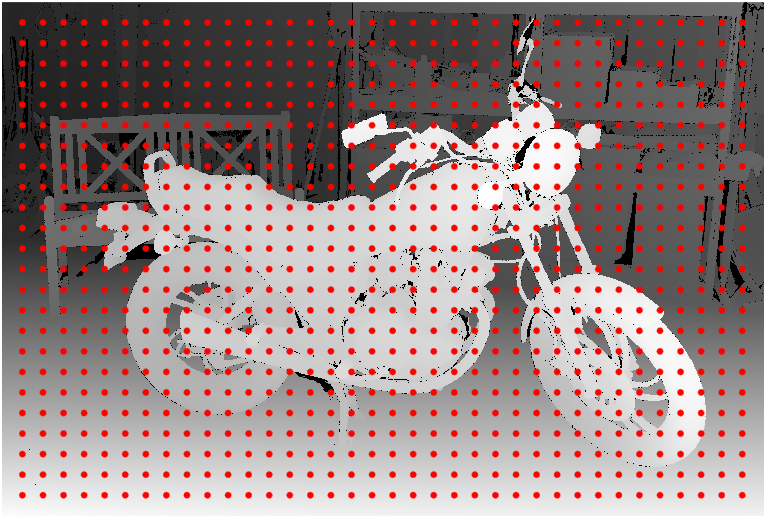
\includegraphics[width=0.4\textwidth, height= 5cm, keepaspectratio]{images/disparity-plus-grid-test-left-01.png}
 		\label{fig:test-matlab-left-01}
}
	\subfigure[Right ground truth stereo test image overlapped by a simulated point grid]{
 		 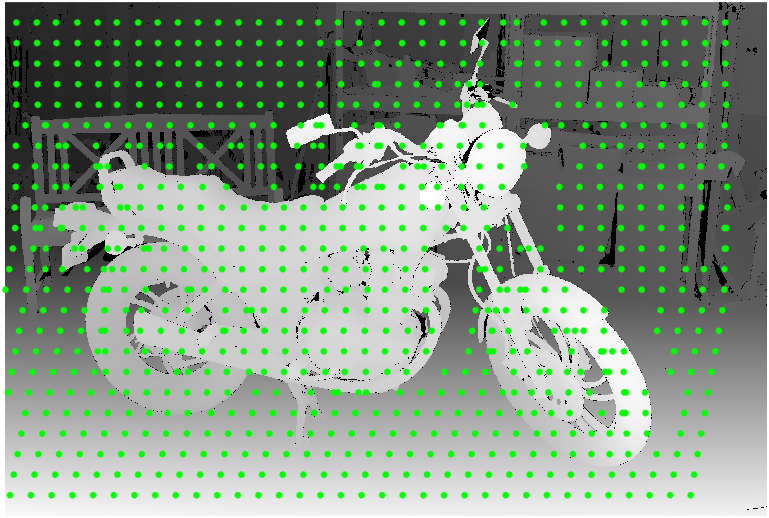
\includegraphics[width=0.4\textwidth, height= 5cm, keepaspectratio]{images/disparity-plus-grid-test-right-01.png}
 		 \label{fig:test-matlab-right-01}
}
\caption{Ground truth images from the Middlebury dataset used for the initial testing phase}
\label{fig:test-matlab-01}
\end{figure}

As anticipated in Chapter~\ref{chapter:methods}, the first phase of the project can be mainly considered as a researching stage.
As a matter of fact, exploiting the stereo images from the Middlebury 2014 dataset, some tests have been performed to obtain an estimation of the feasibility of the conceived idea.\\
Therefore, as Figure~\ref{fig:test-matlab-01} displays, ground truth images have been initially used.
Thus, a point grid, similar to the one generated with the LadiMo device, has been simulated and overlapped to the input images.
In particular, as the difference between Figure~\ref{fig:test-matlab-left-01} and Figure~\ref{fig:test-matlab-right-01} illustrates, to have a reliable simulation of the 3D point cloud generated by the device, the only grid that was actually defined was the one over the principal image, i.e. the left one.
As a matter of fact, as defined in section~\ref{section:stereo-device}, the hardware exploited in the project is provided with only one laser projector.
Therefore, this allows to utilize the produce point cloud only over one image\footnote{Technically speaking the initial cloud of point created through the device can be independently related to both of the image, depending on which is used as the reference one, just applying the correct transformation between the laser system of reference and the reference one}.
After that, those input data, together with the grayscale stereo pair, have been employed in a stereo matching pipeline to recover a disparity map of the analysed scene.\\
In order to acquire useful baseline data regarding the practicability of the thought strategy, tests and analysis over the different areas of the main loop of the algorithm have been investigated.
Actually, this research has been performed with a precise method. \\
First of all the stages of a standard stereo matching method, as defined by Scharstein and Szeliski in \cite{Scharstein2001}, have been separately examined. 
Thus, in order to do this in a reasonable way, the literature regarding both standard and novel stereo matching algorithm has been studied and the main features of the designed algorithm checked out. 
As an example, if the matching cost phase is taken into account, different approaches are presented in the literature for evaluating the similarity among the image pixel values for the respective disparity levels. 
As a matter of fact, as introduced in Chapter~\ref{chapter:background}, the Hamming distance between corresponding pixels can be exploited to determine that measure. 
In relation to that, different algorithms exist to apply a transformation to the input images, making them available for an appropriate implementation of the aforementioned matching cost calculation.
For the actual tests carried out, local methods have been mainly analysed, being more appropriate for the type of data available and for the purposes of the designed strategy.\\
Therefore, as matching cost measures, simple operations have been initially taken into account, such as the sum of absolute differences and the sum of squared differences. 
Moreover, more accurate methods have been later evaluated, i.e. the Rank transform, and its improved version, the Complete Rank transform, broadly discussed in \cite{Demetz2013}.
Then, the Census transform and the Center-Symmetric Census transform proposed by Spangenberg et al. in~\cite{Spangenberg2013} have been investigated.
Considering all of those algorithm, it resulted that the most suitable methods are equivalently the rank and the census transform.
In fact, being these non-parametric transformations, they are not sensitive to changing in lightning inside the environment, thing that usually happen when managing real industrial areas. 
Considering that, at the end the Center-Symmetric Census transform has been chosen because of its reliability, which is comparable to the aforementioned methods, and for the fact that it uses a lower amount of bits to describe the single pixel value compared to the standard Census transform.\\
During this phase of testing, the decision was to run a single pipeline of an \textit{SGM-based} algorithm, whose aggregation cost phase would be based on the four orthogonal directions. 
Moreover, another operative choice was to use the whole image for the complete execution of the designed method.
Therefore, it was thought that, at least for this researching phase, it would be meaningless to define a hierarchical implementation of the code, where the image is initially downscaled and subsequently scaled up again in order to make the execution faster, as made by Hermann and Klette in their application of the Semi-Global Matching algorithm \cite{Hermann2013}.\\
At the end of this \textit{research} section of the project, the results did not show an exact path to follow. 
Specifically, the disparity image obtained was actually lower in accuracy compared to the method implemented in MATLAB by Eric Psota and available at the website of the Middlebury stereo dataset \footnote{\href{http://vision.middlebury.edu/stereo/submit3}{links Middlebury College Stereo}} and to the MATLAB built-in method \textit{disparitySGM}. 
Moreover, the developed implementation was quite slow, if correlated to the benchmark of most of the standard SGM-based methods. \\
However, some considerations should be proposed regarding that outcome. 
First of all, the algorithm designed runs iteratively, that is no parallel loop is coded to make the execution faster.  
This is, in fact, explained by the decision of being interested in the relative performance among the own designed methods. 
Furthermore, any sort of GPU enforcing was used. 
Hence, it was quite expected to not obtain good performance.
On the contrary, the thought strategy was evaluated as feasible and, additionally, the exploiting of proper initial data provided by the stereo camera would likely be an enhancement to the overall performance of the algorithm. \\

\section{Derivative based method implementation}
\label{section:derivative-based}

Verified the feasibility of the considered strategy, the project design shifted to the actual algorithm development. 
Therefore, exploiting the OpenCV libraries and using the images from the Middlebury 2014 dataset, the derivative based method started to be implemented in a C++ code. \\
In this initial phase of its designing, the simulated grid based on the ground truth images was still used as the method to obtain the input point cloud data.
As a matter of fact, the only practical advantage of employing such simulated data stands on the amount of noise that they contain.
As a matter of fact, an appropriate comment to that strategy would be that, once the real data from the device would be used, the result would be probably be worse in terms of overall accuracy. 
Anyway, at that initial stage of the algorithm development, the interest was focused on comparing the performance of the pure SGM-based and the derivative-based implementations. \\

\subsection{General features of the method and simulated grid specifications}
\label{subsection:general-feature-der-method}

\begin{figure}[t]
	\begin{center}
		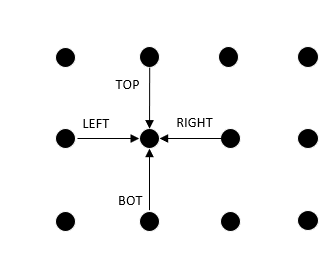
\includegraphics[width=.8\textwidth, height=5cm, keepaspectratio]{images/grid-subwindow-detail}
\caption{Detail of a point grid patch where a set of neighbouring points is highlighted}
\label{fig:grid-subpatch}
	\end{center}
\end{figure}

\begin{figure}[t]
	\begin{center}
		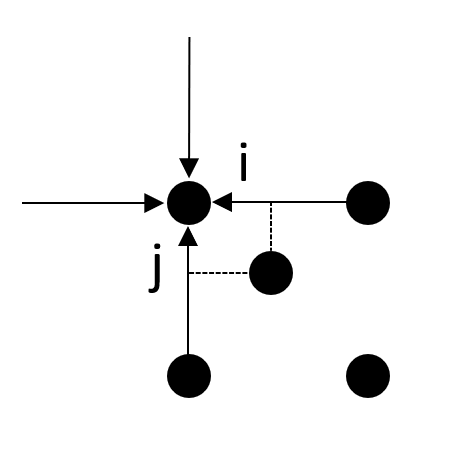
\includegraphics[width=.8\textwidth, height=5cm, keepaspectratio]{images/point-estimation-detail}
\caption{Detail of a point grid patch where the estimation of a new point at relative coordinates $i$ and $j$ is performed}
\label{fig:subpatch-estimation}
	\end{center}
\end{figure}

The so called derivative-based method, which arises to be both efficient and generally accurate, based its strength on the sparse point cloud gained through the structured light stereo camera.\\
The main features of that algorithm are now precisely described.
Moreover, attention is focused on the conventions utilized to define the main parts of the method and on the functions created for obtaining the 3D point estimations over the initial laser grid. 
Subsequently, some fundamental sections of the designed implementation are more broadly described, thus to provide to the reader a complete understanding of the work done. \\
For this reason, the analysis starts by considering a simulated grid of points, which was defined in the C++ code in order to initially mimic the real laser grid generated by the LadiMo device. 
This approach, as aforementioned, does not invalidate the outcome obtained through all the designing process of the method.
Instead, it is a reasonable strategy for achieving some initial temporary results, which can then provide a guidance to the following phases of the whole process.\\
Therefore, let us consider the entire point cloud as a regular grid where each point is defined by its coordinate in the space.
Additionally, it can be also thought that the corresponding 2D coordinates in the reference image plane can be easily retrieved using the camera matrices.
Hence, if a neighboring set of four points is taken into account, as highlighted by Figure~\ref{fig:grid-subpatch}, the local derivative vectors for all the considered coordinates can be easily calculated.
This estimation of the derivative is extremely useful for the following reasons.
First of all, they are, actually, exploited to generate the estimations inside each grid sub-region.
Moreover, they can be employed to evaluate if, inside the specific patch of points, there could be an edge of some shape. 
In this latter case, the magnitude of the Z component of the derivative vector will, in fact, be higher than a set threshold, which can be defined looking at the average values of the Z coordinate of the grid points.\\
Therefore, explaining the project design procedure implemented, it can be summarized as follows.
Initially, for each one of the points in the grid the derivatives have been calculated with respect to its four neighbors, as the rows in Figure~\ref{fig:grid-subpatch} underline. 
This means that each point will have, then, four distinct set of local derivatives, conventionally defined as follows:
\begin{itemize}
	\item \textbf{from top:} derivative between the specific point and its top neighbor;
	\item \textbf{from boottom:} derivative between the specific point and its bottom neighbor;
	\item \textbf{from left:} derivative between the specific point and its left neighbor;
	\item \textbf{from right:} derivative between the specific point and its right neighbor.
\end{itemize}
In these definition a neighbor to a point is defined with the subsequent rule. 
Let us consider a point, which is classified through the grid coordinates $r$, along the row grid direction, and  $c$, along the column direction. 
Its neighboring points are, hence, identified by:
\begin{itemize}
	\item \textbf{top} neighbor: with coordinates $r - 1$ and $c$;
	\item \textbf{bottom} neighbor: with coordinates $r + 1$ and $c$;
	\item \textbf{left} neighbor: with coordinates $r$ and $c - 1$;
	\item \textbf{right} neighbor: with coordinates $r$ and $c + 1$;
\end{itemize}
Using that scheme the four derivatives estimated for each point will contain the difference between the actual point  \textbf{\textit{full location components}} and the ones of the relative neighbor regarding.
In the implemented code, the introduced \textbf{\textit{full location components}} are in the order: the $x$ and $y$ components of the point projected in the principal image plane, therefore they are measured in pixels, the $X$, $Y$ and $Z$ space coordinates of the point, in meters, and finally, $d$ is the disparity value, in pixel, related to the depth of the point, which can be evaluated through equation~\ref{eqn:disparity-depth}.\\
Therefore, let us now consider to estimate an unknown point inside a subregion of the whole grid, that was decided to be identified by 4 points, as Figure~\ref{fig:subpatch-estimation} displays.
The final 3D coordinates of the new point will be, at first, defined by four different estimations, each one related to the four corners of the grid subwindow, as follows.

\begin{subequations}
\label{eqn:point-patch-estimation}
	\begin{align}
		est_{TL} = TL + i \cdot der_{from-left} + j \cdot der_{from-top} \\
		est_{TR} = TR + (i-1) \cdot der_{from-right} + j \cdot der_{from-top} \\
		est_{BL} = BL + i \cdot der_{from-left} + (j-1) \cdot der_{from-bottom} \\
		est_{BR} = BR + (i-1) \cdot der_{from-right} + (j-1) \cdot der_{from-bottom}
	\end{align}
\end{subequations}

where $TL$, $TR$, $BL$ and $BR$ respectively point to the estimation done with respect to the top-left corner of the grid sub-window, the top-right corner, bottom-left and bottom-right corner. 
Then, $i$ and $j$ are the relative $x$ and $y$ coordinates of the estimated point, whose values range between 0 and 1.
Finally, in the notation employed, $der_{dir}$ stands for the different derivative vectors related to each corner point and visualized by the arrows in Figure~\ref{fig:subpatch-estimation}. \\
Once, these estimations are achieved exploiting the derivatives, as equations in~\ref{eqn:point-patch-estimation} define, the best evaluation is obtained by calculating each matching cost between the corresponding pixels between the stereo images. 
The matching cost is determined following the subsequent routine.\\
In relation do this, it should be reported that, due to the researching aspect of this project, lots of changing have been made to the code.
Therefore, to provide a clear explanation of the decisions made and the procedure followed, which, otherwise, could appear sometimes winding, all the relevant changing to the functions used are disclosed. 
Beside this brief comment about the created code, the best, among four, estimation of the new grid point is such evaluated.\\
The estimation provides the values of the 3D coordinates of the calculated point and its disparity.
The point location is, then, projected through the camera matrix to the reference image (usually the left image) pixel coordinates and the corresponding position in the support image is determined using the estimated disparity value. 
At this point the matching cost is computed as the absolute difference between the intensity values of the analysed pixels in the left and in the right image planes. 
However, this kind of measure appears to give weak results. 
As a matter of fact, the main problem was that, in some situations, the estimation labelled as the best one actually contained a value of disparity doubtful, if compared to the one of the point's closest neighbours.  
Moreover, this generally happened in textureless regions, where it is obviously more difficult to make accurate estimations.\\
To overcome this problem, a penalty value was added to each partial estimation. 
Moreover, that value was weighted linearly basing on the distance between the estimated point and the corresponding corner. 
In this manner, the estimation, related to the disparity and to the coordinate values of the closest corner, is most likely to be addressed as the best one.
Once the best estimation for each new point is calculated, the evaluated values of the 3D point coordinate are processed, applying a morphological filter, in order to remove undesired noise and smooth out the overall data. \\
The estimation procedure just described is not actually able to handle all kind of situations, concerning the provided input objects.
In fact, incorrect values used to be estimated in sub-regions affected by edge features, and thus occlusions. \\
Therefore, to correctly manage these situations, multiple cases have been defined, regarding the edge cases. 

\subsection{Edge cases and penalty values discussion}
\label{subsection:edge-cases-and-penalties}

At first, four main conditions have been distinguished. 
These comprise the possibility to do not have any type of edge inside a grid subregions, the existence of a vertical edge in the patch, an horizontal edge case and finally a so called \textit{undefined} case has been defined.\\
Therefore, in each one of these situations, the point estimation procedure differs slightly, so that the aforementioned linear penalty can be more wisely set.
Regarding this two distinct values of the penalty have been employed, a lower and a higher value.
In fact, because it is not efficiently possible to correctly estimate the position of the potential edge, the choice of the correct estimation has to be somehow driven by exploiting the linear penalties. \\
Moreover, to identify the correct type of edge, the derivatives have been exploited and, specifically, the magnitude of the $Z$ component of the vector. 
Basically, a general edge case, which is equivalent to the \textit{undefined} condition, is initially determined by computing the absolute difference between the $Z$ components of all the possible couples of corners, i.e. the $Z$ value of the local derivatives, and comparing that with a pre-determined threshold, which is related to the average depth value of the initial points of the grid. \\
Therefore, during the algorithm pipeline, the possibility of having an edge feature inside the specific patch is initially checked.
Then, if the depth values of the four corner are almost equivalent, this means that the area is actually planar.
Thus, in this situation, a fast interpolation method is run, so that the overall computation can be even faster.\\
On the contrary, if a vertical or an horizontal edge is found, the small and big penalties are used accordingly.
For example, if the edge is vertical, the small penalty will be multiplied to the relative $y$-coordinate of the estimated point, instead the big penalty will weight the $x$-coordinate.\\
Finally, for the undefined case, the penalty weight is equivalent in both directions, $x$ and $y$, and its magnitude ranges between the two previously defined penalties. \\
Those three different edge cases are the one initially tested. 
However, later appeared that a more meaningful strategy should be based on the definition of two grater categories, which would comprise the cases described above.
These two bigger classes describe, thus, \textbf{soft} and \textbf{strong} edges. 
In fact, results of tests done with dataset images show that employing a single threshold for the depth difference and focusing only over the edge direction was not entirely correct. 
As a matter of fact, in a generic scene different types of objects exists. 
Therefore, adapting the edge analysis to the object distances, for example between the whole foreground and the background and between multiple objects of the foreground, that would give a smoother and more accurate dense 3D point cloud.

\subsection{Derivative computation and sanity check}
\label{subsection:derivative-computation}

The core of the estimations are, actually, the local derivatives computed for each point of the grid. 
Basically, each grid point contains four vectors, which are the local derivatives between the reference point and its four orthogonal neighbors. \\
Initially the mere derivatives have been calculated as pointing towards the reference point, like Figure~\ref{fig:grid-subpatch} shows. \\
However, it came out that this procedure was not enough accurate, to generate a proper dense 3D point cloud.
Therefore, a \textit{sanity check} has been later defined inside the derivative calculation pipeline to achieve preciser computation of the local derivatives, especially for the grid sub-patches where edges are likely to be found.\\
Moreover, a higher accuracy of the final result has been achieved when evaluating, for each grid point, two slightly different types of derivative vectors.
Specifically, \textit{internal} and \textit{external} derivatives. 
This distinction allowed to achieve faster and more accurate results, especially when dealing with edges in the grid sub-region. 
Precisely, if the presence of an edge is verified for the considered patch, the external (with respect to the sub-window) derivatives were used.
Otherwise, exploiting the internal derivatives the computation could be made faster, being them equal in couple among the corners of the patch. \\
Referring to what introduced at the end of Section~\ref{subsection:edge-cases-and-penalties}, in the latest implementation designed, the estimation process is driven by the edges analysis. 
As aforementioned, the test results demonstrate that a distinction based only upon the edge shape is not enough to reach a good degree of accuracy.
Therefore, the analysis cases have later been defined basing on the strength of the edges between the objects in the scene.\\
Hence two different thresholds have been so determined. 
The first is used to identify occlusions that basically occur between foreground objects and the background. 
These have been designated as \textbf{\textit{strong}} edges. 
Differently, the other case is specified as the \textbf{\textit{soft}} edges case.
This is related to occlusions happen between parts of the same object at different values of depth, as could be between the chin and the neck of a person.\\
Moreover, on top of this first level of edge selection, the following cases have been then defined, which are correlated to the specific value of the penalty.
Precisely, they are \textit{pure vertical} and \textit{pure horizontal} edges, for which it should happen that the depth values of the corners are equals in couple.
Then, there are some particular cases, which have the scope of leading the disparity estimation of the new point in a more accurate way.
They are: \textit{diagonal top left}, \textit{diagonal top right}, \textit{diagonal bottom left}, \textit{diagonal bottom right}.
Furthermore, there is the undefined case, which is triggered when the potential edge found in the subregion has a strange shape.\\
Taking now into account the actual estimation functions, these are slightly different for the aforementioned edge cases identified.
Summing up the overall procedure, it can be said that, the main distinction, which guides the whole process is the first one, that is the one that distinguish among, strong, soft and no edges.
Then, for all the subcases, the main difference stands on the values and order of the penalties. \\
Hence, in the \textit{no edges} case, four temporary estimations are performed for each new grid point by carrying out a linear interpolation, which exploit the \textit{internal} derivative vectors.
Then, for the other two main cases, the procedure is generally the same. 
In fact, the fundamental function of distinguish between those types of occlusions is to make the final outcome smoother. \\
Thus, when dealing with edges, at first the algorithm checks for each temporary estimation, that is for each subregion corner, if there could also be edges in the neighborhood outside of the region. 
If this is false, a linear interpolation is computed employing the \textit{external} derivatives.
Otherwise, the interpolation is done with the \textit{internal} derivatives and only for the $x$ and $y$ pixel positions. 
Therefore, the depth value is matched with the one of the corresponding corner, thus to enhance the smoothness of the final result.

\section{Semi-Global Matching based method implementation}
\label{section:sgm-based}

The other implemented method based on the initial grid of points follows more closely the standard stereo-matching structure.
Moreover, it does not distinguish between \textbf{\textit{strong}} and \textbf{\textit{soft}} edges, but the different cases are identified only considering the shape of the potential edge present inside the subwindow. \\
Therefore, this algorithm initially computes the \textit{matching cube cost} for the specific grid patch. 
The difference between the standard SGM method stands on that cube, whose third direction does not generally contains continuous values of the disparity.
On the contrary, those values are defined by the sub-window corners, whose disparity define the levels of the cost cube.\\
Therefore, if no edge is found, only the matching cost part of the stereo matching algorithm is carried out.
Otherwise, the aggregation cost phase is implemented.
In this latter case, the cost is actually aggregated only on the direction orthogonal to the shape of identified edge.\\
At the end of the pipeline simple post-processing operations are performed over the obtained data, as done for the other algorithm.
Considering the overall method, it result to be give a denser point cloud compared to the previous method. 
However, it computational time is extremely higher.
This is clearly due to the fact that this algorithm estimates each single pixel inside the specific subregions.
Contrarily, in the \textit{lightweight} strategy the number of samples that the user wants to estimate can be adjusted. 
In this way the trade-off between accuracy and resources utilization can be externally defined. 

\section{OpenCV built-in Semi-Global Box Matching algorithm}
\label{section:opencv-sgm-method}

\section{Pre-processing testing and analysis}
\label{section:pre-processing-impl}

The pre-processing phase can be ideally divided in multiple parts.
First of all, general operations have been applied for both estimation methods in order to remove noisy components from the stereo pair and from the ground truth images, when exploiting the simulated grid for the estimations.
Then, a section of the pre-processing phase can be considered the importing of all the necessary calibration data and the creation of a sort of look-up table, which was used together with the grid of points.\\
On the contrary, when working with the real data coming from the LadiMo stereo device, some initial operations have been necessary to clean up \textit{bad} point values and for estimating some of the missing data, which would be determined without losing in accuracy. \\
Regarding the image pre-processing, different noise removal filters have been tested over database images, in order to understand which would provide the best trade-off in most of the cases. 
Median and bilateral filters appear to be, almost equivalently, the best choice for smoothing away the noise while loosing the smallest amount of information from the input images. \\
Considering the others pre-processing operations implemented in the algorithm, they depend on the condition of working or not with the simulated grid.

\subsection{Look-up table and point grid pre-processing}
\label{subsection:grid-preprocessing}

Therefore, for the initial testing phase of the algorithm designing, when multiple tests have been carried out using the images from the Middlebury dataset, a look-up table has been defined in order to ensure a fast data finding. 
This structure has been easily built by progressively numbering the simulated gridpoints, so that their values correspond to the row index of the data matrix. \\
Considering the real data, instead, the two main initial operations that have been defined in the pipeline regard data analysis. 
As a matter of fact the laser grid data are not entirely perfect.
Contrarily, for the of the points the 3D data are completely missing.
This generally happen close to the edges and it is most likely due to occlusions and shadows.
Moreover, the used device has some lack of performance when dealing with relatively small objects. 

\subsection{Image undistortion and rectification}
\label{subsection:img-undist-and-rectific}

\section{Post-processing testing and analysis}
\label{section:post-processing-impl}

\section{Preparation to future improvements}
\label{section:intro-future-improv}

%
%\chapter{Evaluation and Results comparison}
\label{chapter:evaluation}

In the previous chapters the description of the methods and of the key sections of the designed algorithms has been carried out.
In Chapter~\ref{chapter:methods} a general outline of the implemented idea has been presented.
Instead, Chapter~\ref{chapter:implementation} illustrates the key functions and the computations that build up the entire algorithm.\\
Therefore, the functions exploited in the pre and post-processing phases have been previously outlined. 
Moreover, the two novel strategies designed have been reported, underlining the procedure implemented for obtaining the estimations of the grid points, the matching cost methods tested and their efficiency throughout the algorithm and the correlation with previously created stereo matching algorithms. 
Chapter~\ref{chapter:methods} contains also a brief presentation of similar ideas developed in standard and in deep learning based methods, which were exploited to obtain an initial proof of the potential performance of the algorithm.\\
Thus, this chapter delineates the results obtained supporting the discussion with images of the point cloud and the disparity maps obtained.
Moreover, some general comments related to the different result are going to be presented.
In fact, a discussion focused on the considerations that can be carried out from the outcomes obtained will cover Chapter~\ref{chapter:discussion}.\\
Here the interest is centred on the results achieved and in the comparison between the OpenCV method, defined as the baseline, and the algorithms designed.
Moreover, in the first part of the following analysis the outcomes collected during the initial phase of the whole work are proposed.
As previously introduced, their main function was to provide, at the beginning of the developed project, a proof of the feasibility of the thought strategy. 
That was, in fact, extremely useful for having, from the very beginning, a qualitative guidance on the project development. 

\section{Researching phase results}
\label{section:research-phase-results}

\begin{figure}[t]
	\centering
	\subfigure[Left RGB test image]{
 		\includegraphics[width=0.4\textwidth, height= 5cm, keepaspectratio]{images/left-playtable-test.png}
 		\label{fig:test-matlab-left-02}
}
	\subfigure[Right RGB test image]{
 		 \includegraphics[width=0.4\textwidth, height= 5cm, keepaspectratio]{images/right-playtable-test.png}
 		 \label{fig:test-matlab-right-02}
}
	\subfigure[Disparity test image]{
	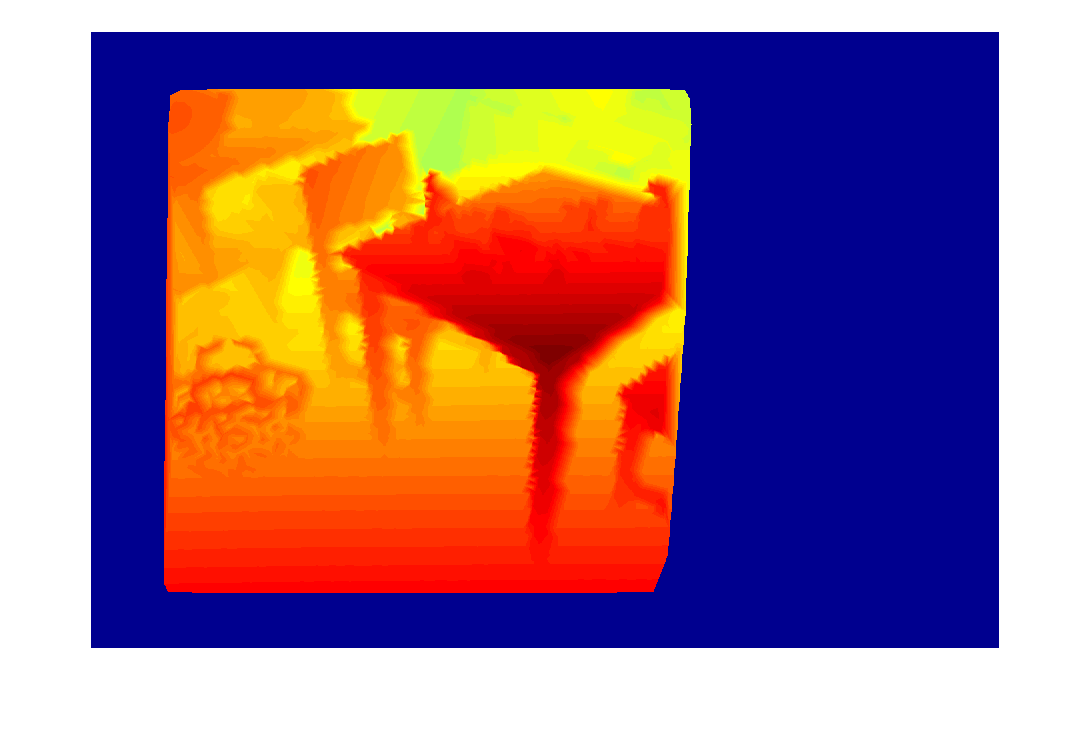
\includegraphics[width=0.8\textwidth, height=5cm, keepaspectratio]{images/disparity-map-playtable-test.png}
	\label{fig:disparity-test-02}
}
\caption{Test images from the Middlebury 2014 dataset with disparity image estimated with linear simple semi-global matching based method to test feasibility of thought strategy}
\label{fig:test-matlab-02}
\end{figure}

Figure~\ref{fig:test-matlab-02} displays the result of the estimation of a disparity image exploiting a stereo pair from the Middlebury 2014 dataset.
The disparity map shown in Figure~\ref{fig:disparity-test-02} has been achieved applying a rather simple and linear implementation of a semi-global based method, where information from an initial simulated sparse grid of point is employed.
As a matter of fact, in that initial stage of the project designing, the overall performance was not taken into account.
The main focus was the feasibility of the procedure compared to standard SGM-based algorithms. 
In fact, the core of the algorithm computations stand in the matching cost phase, which is based on the Center-Symmetric Census transform and on the Hamming distance computation.
Then, the aggregation cost step is carried out only over the four main orthogonal directions.
Finally, a basic left-right consistency check procedure is applied, which generate the lost of information of the two image sides.
Clearly, this behaviour is related to the disparity range employed in the algorithm.

\section{Derivative method results}
\label{section:der-method-results}

\begin{figure}[t]
	\centering
	\subfigure[Derivative-based method]{
 		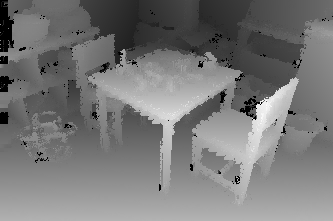
\includegraphics[width=0.4\textwidth, height= 5cm, keepaspectratio]{images/raw-disparity-playtable-test.png}
 		\label{fig:derivative-based-test-table}
}
	\subfigure[SGM-based method]{
 		 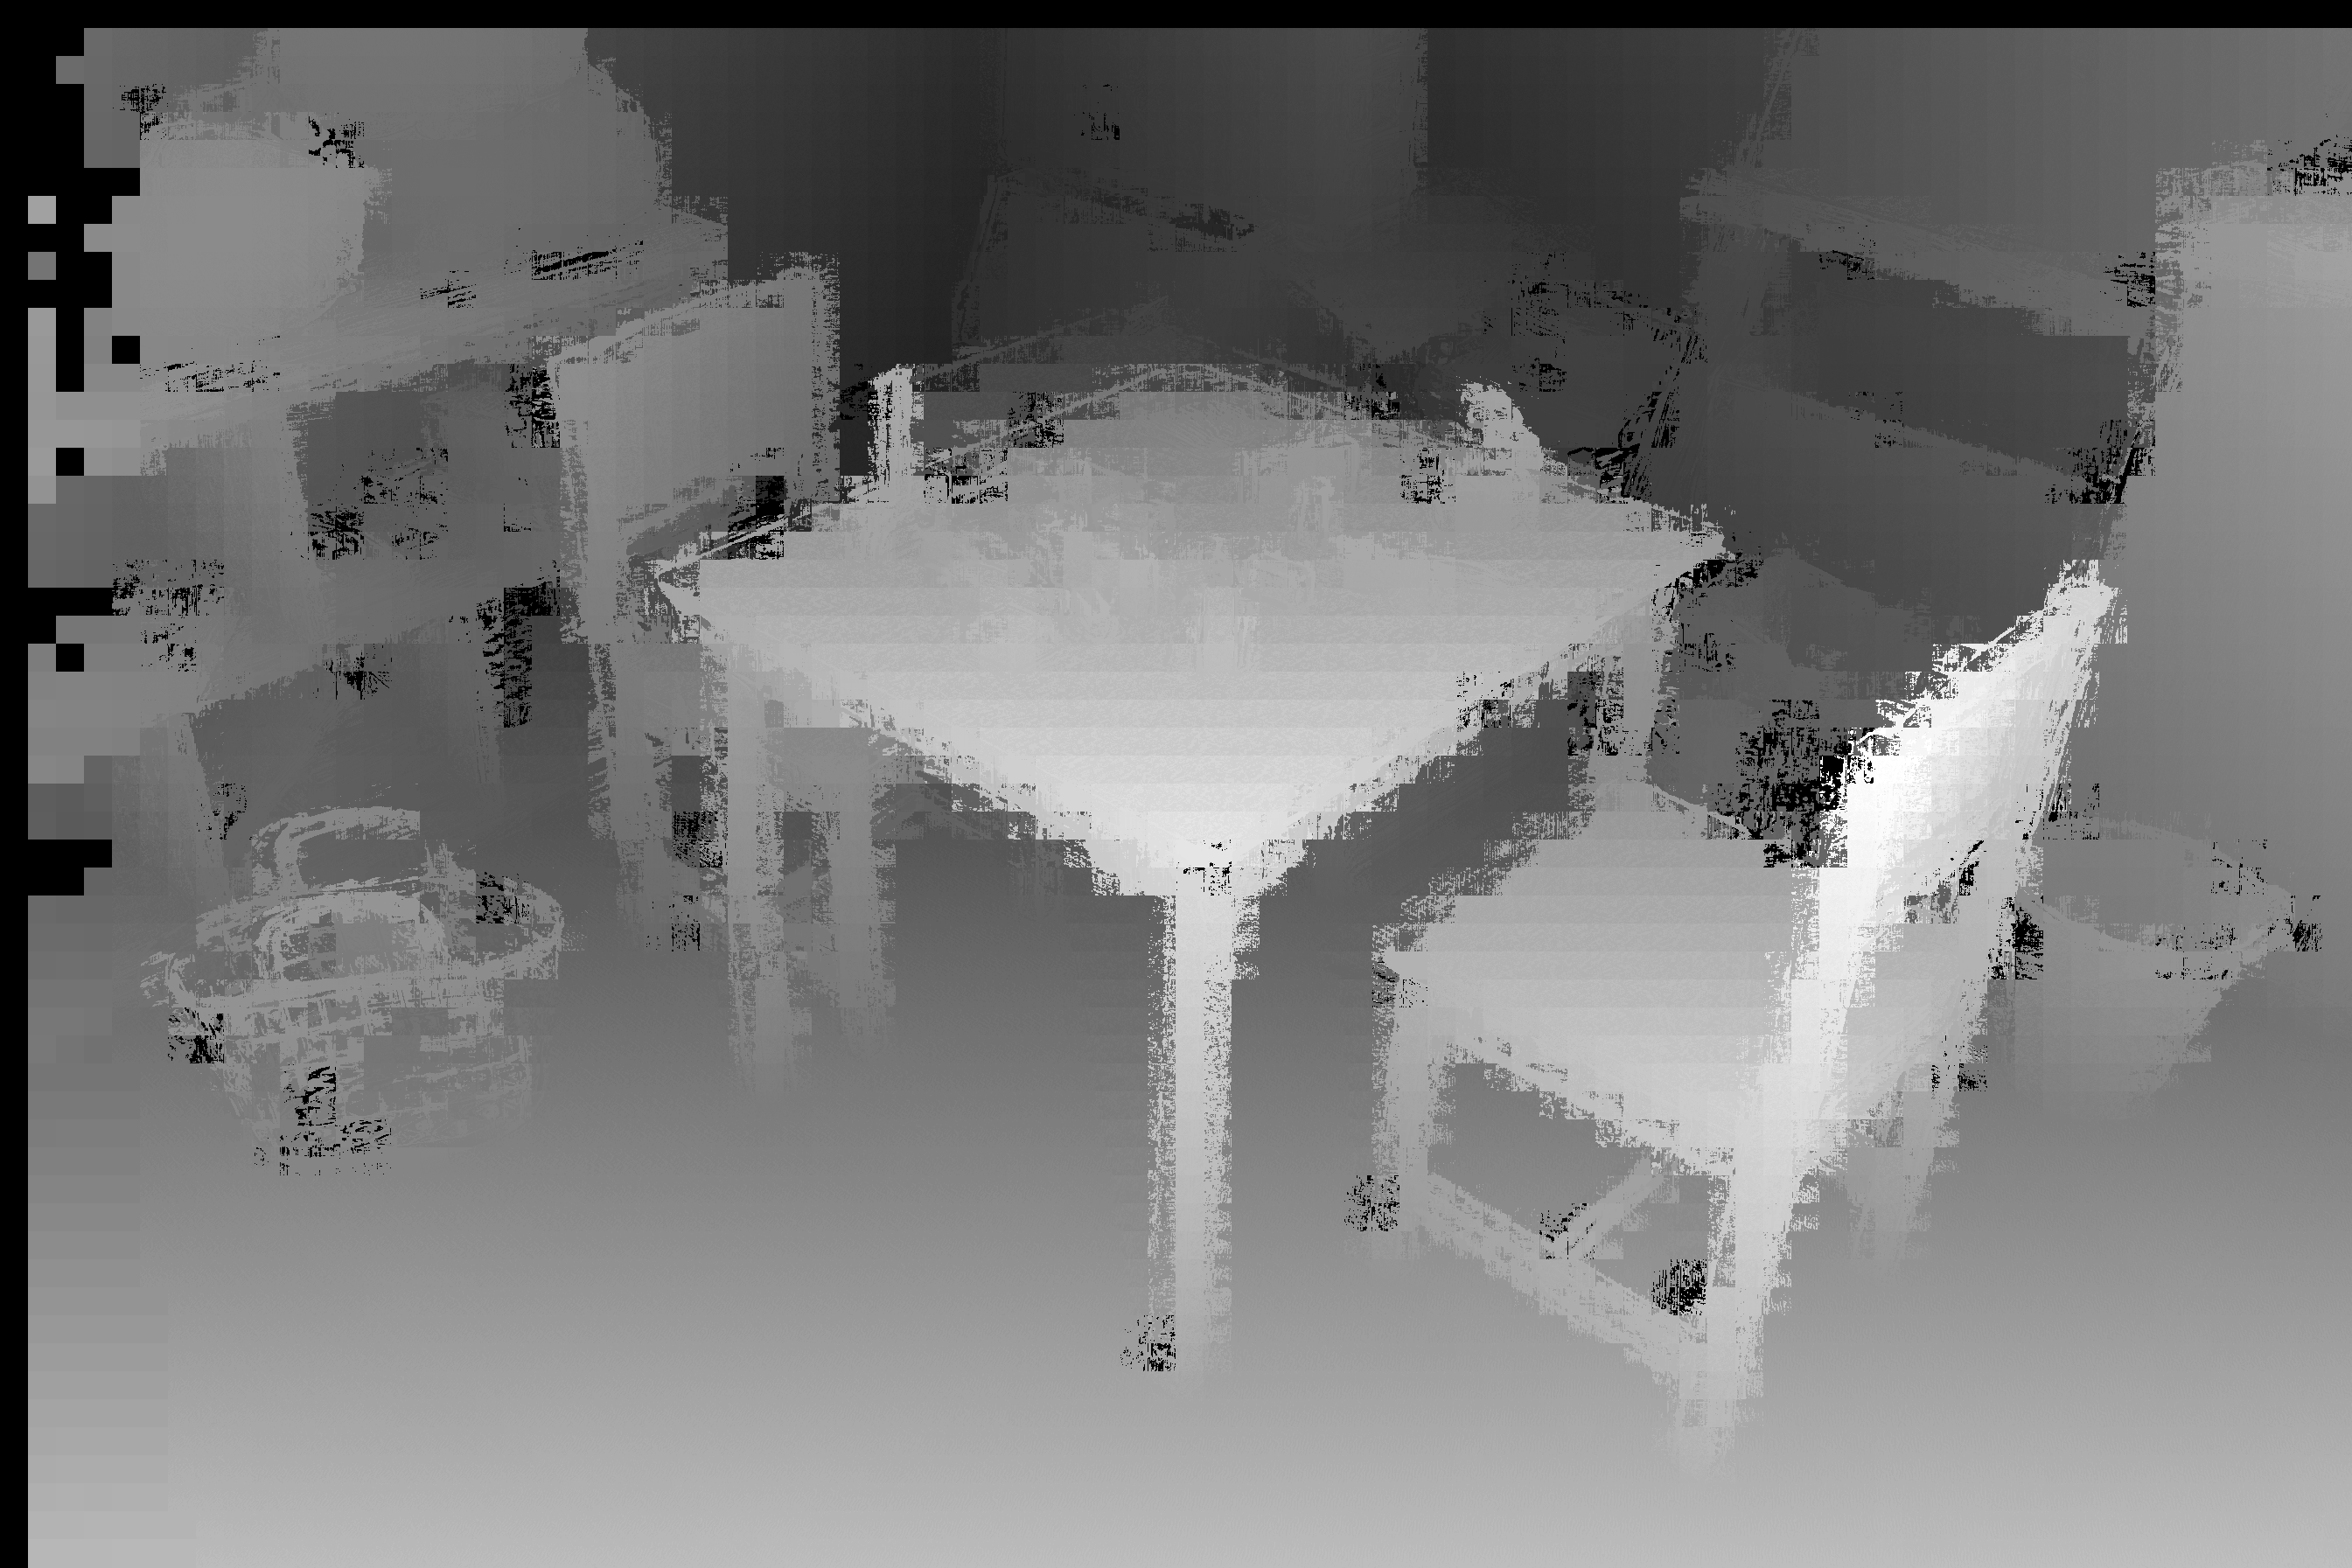
\includegraphics[width=0.4\textwidth, height= 5cm, keepaspectratio]{images/sgm-based-playtable-test.png}
 		 \label{fig:sgm-based-test-table}
}
	\subfigure[OpenCV stereoSGBM method]{
	 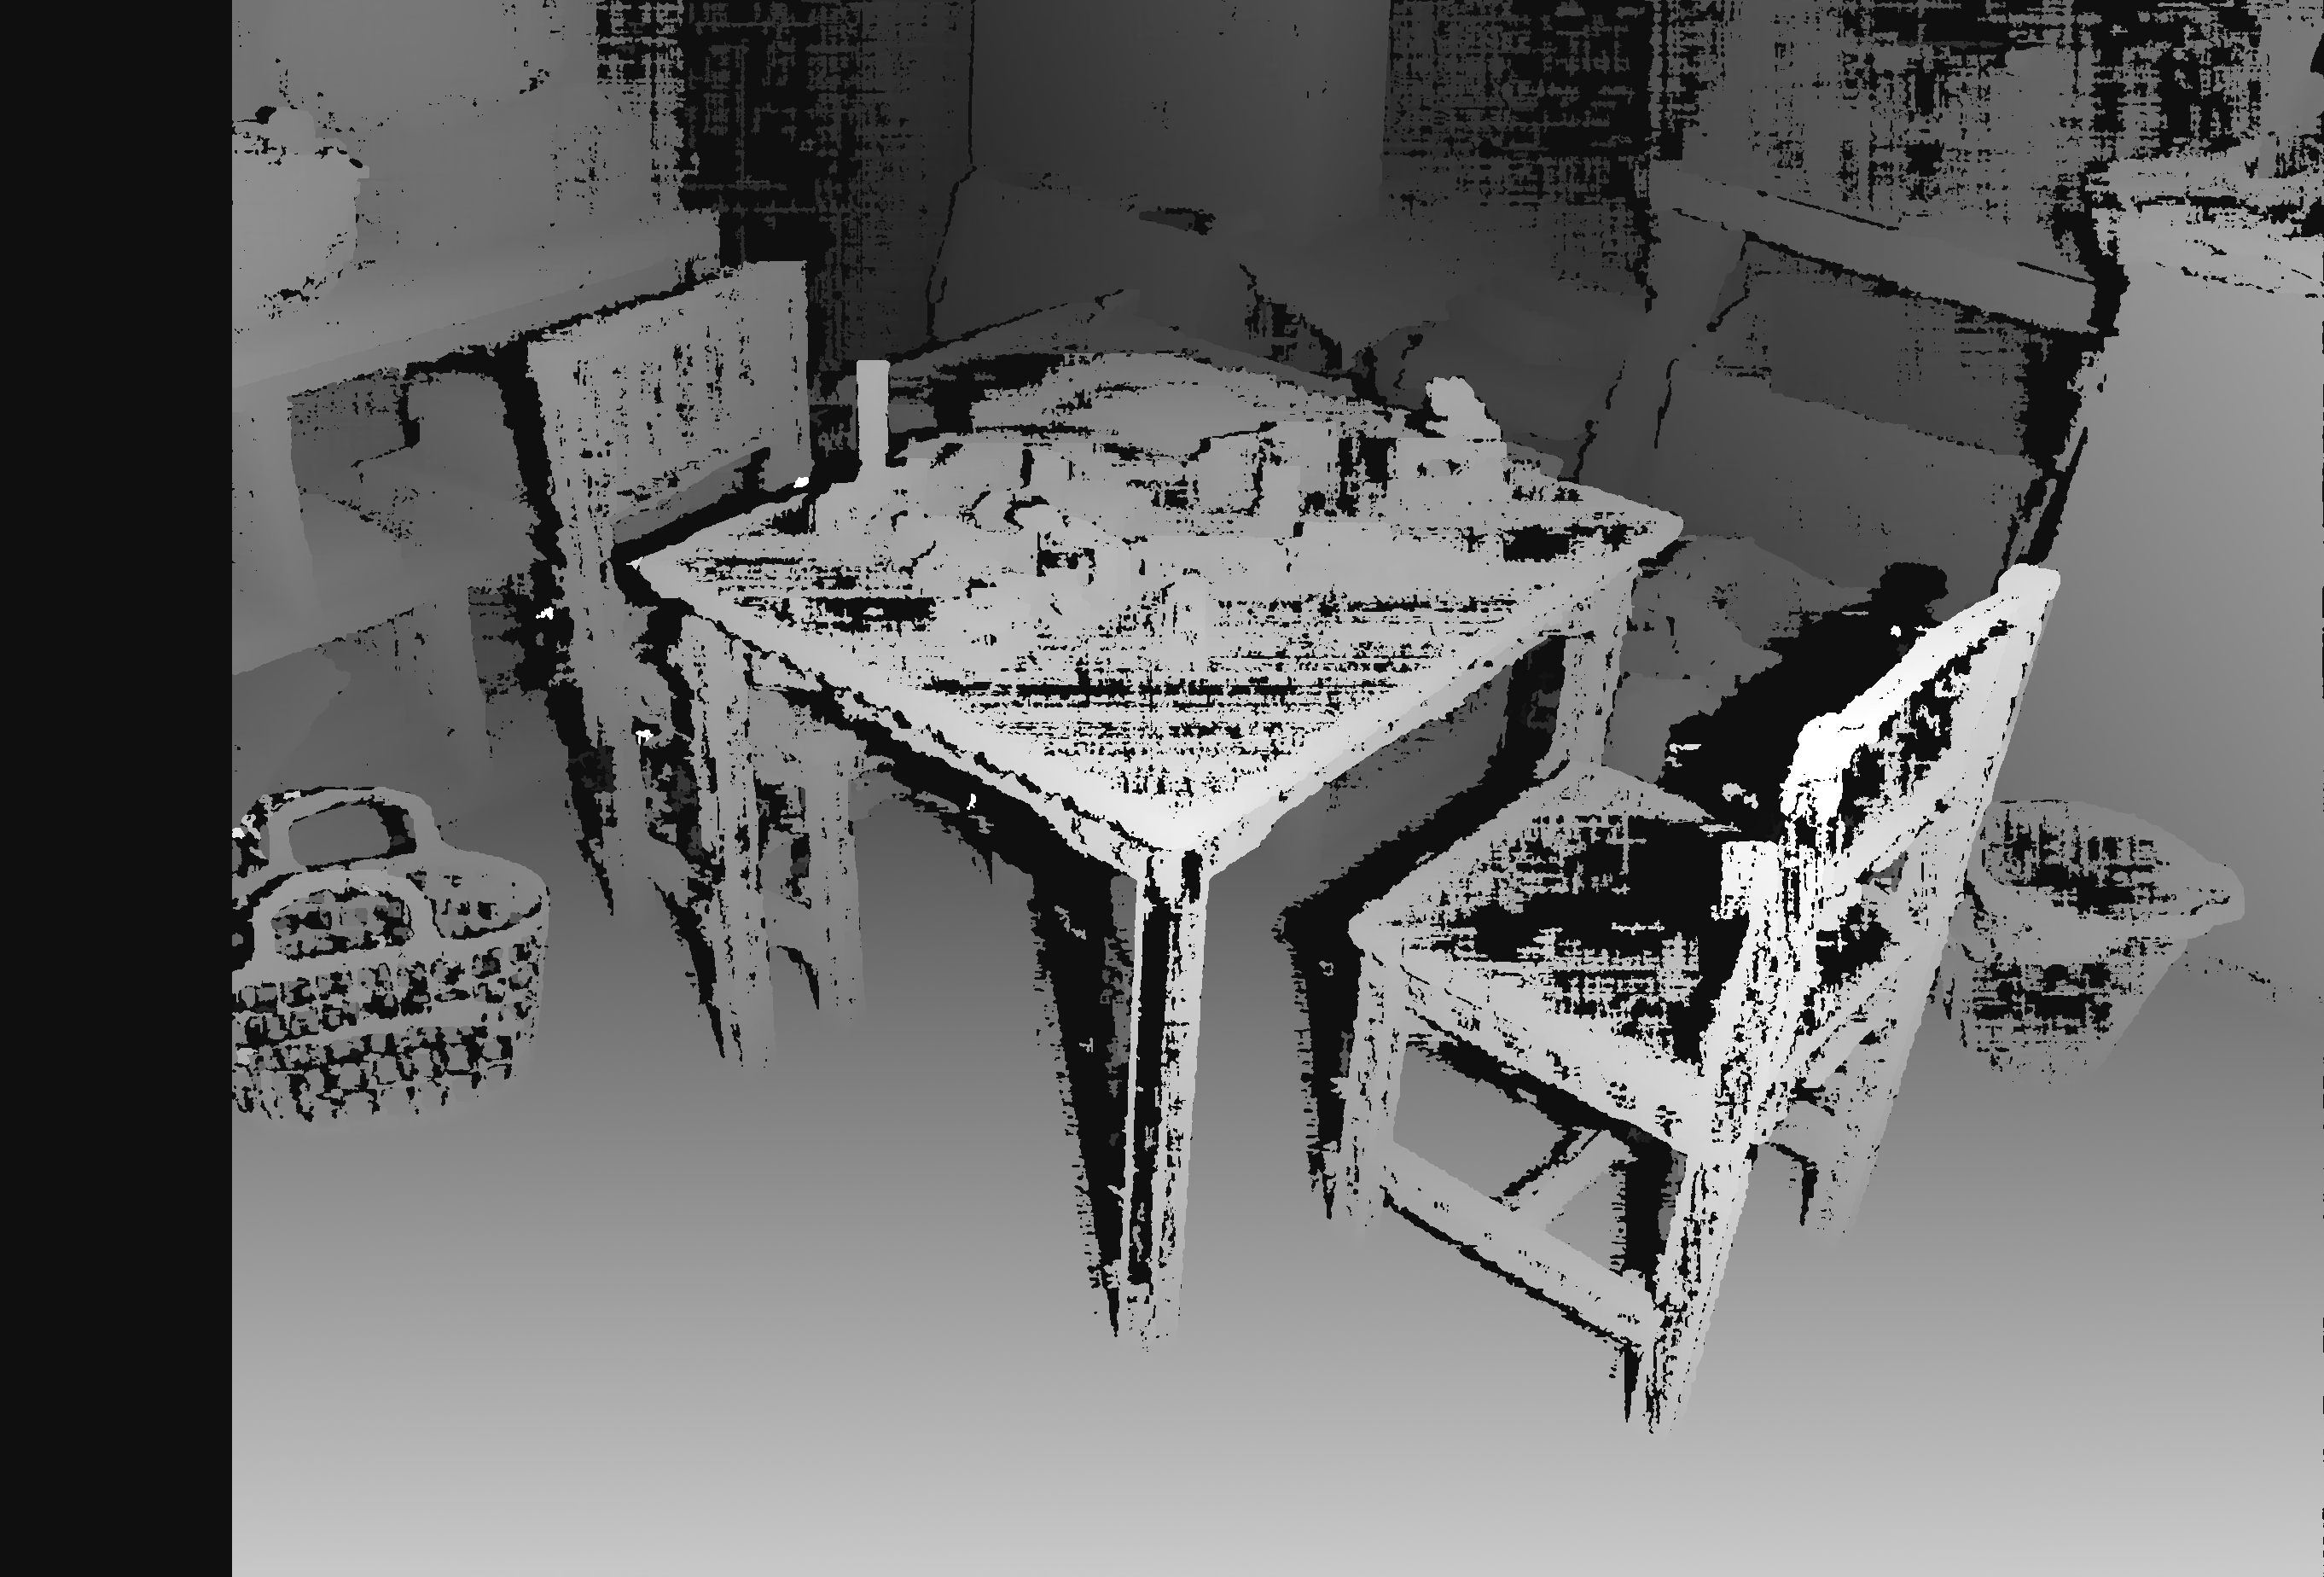
\includegraphics[width=0.8\textwidth, height= 5cm, keepaspectratio]{images/opencv-baseline-test-playtable.png}
 		 \label{fig:opencv-baseline-test-table}
}
\caption{Results of disparity images obtained with the disparity-based lightweight method, the SGM-based method and the baseline result from the OpenCV built-in method}
\label{fig:test-novel-methods-table-01}
\end{figure}

\begin{figure}[t]
	\centering
	\subfigure[Input left raw image ]{
 		\includegraphics[width=0.4\textwidth, height= 5cm, keepaspectratio]{images/stereo-rectified-left-16bit.png}
 		\label{fig:raw-image-4eye-der-method-left}
}
	\subfigure[Input right raw image]{
 		 \includegraphics[width=0.4\textwidth, height= 5cm, keepaspectratio]{images/stereo-rectified-right-16bit.png}
 		 \label{fig:raw-image-4eye-der-method-right}
}
	\subfigure[Input point cloud]{
	 	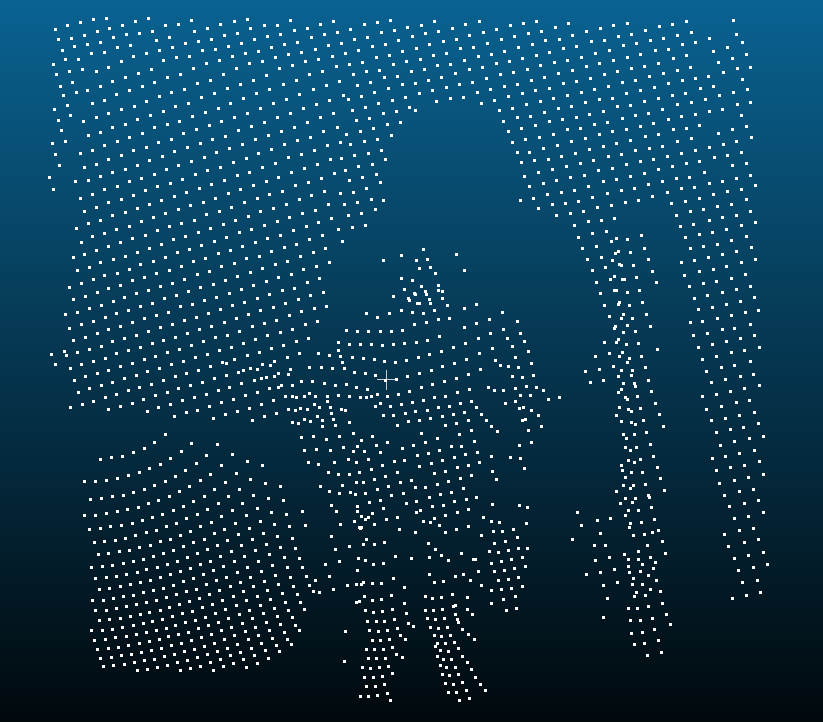
\includegraphics[width=0.4\textwidth, height= 5cm, keepaspectratio]{images/point-cloud-4eye-input.png}
 		\label{fig:input-point-cloud-4eye-der-method}
}
	\subfigure[Output dense point cloud]{
	 	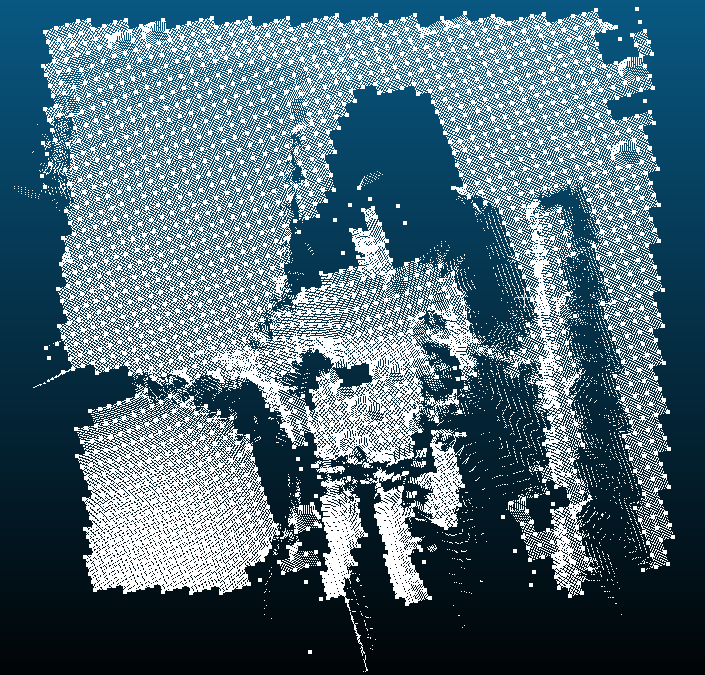
\includegraphics[width=0.4\textwidth, height= 5cm, keepaspectratio]{images/estimated-and-initial-points.png}
 		\label{fig:output-point-cloud-4eye-der-method}
}
\caption{Pair of raw images from the LaDiMo device, initial grid of point and final point cloud estimated with derivative-based method}
\label{fig:result-4eye-derivative-method}
\end{figure}

As Figure~\ref{fig:disparity-test-02} proved, it is possible to achieve reasonable results with the designed method.
However, the interesting thing is that, the initial tests performed show that, exploiting a sparse enough grid of points, which carry information on their 3D positions, the overall implementation can be made faster.\\
Therefore, after the initial researching phase, the algorithm started to be implemented in C++, in order to have a faster execution with respect to MATLAB, employing functions from the OpenCV library.
In this regard, Figure~\ref{fig:test-novel-methods-table-01} presents the grayscale disparity image achieved by applying the two designed methods, the derivative-based one and the SGM-based one, and then the outcome of the OpenCV built-in method is proposed as baseline for a visual comparison.\\
Therefore, considering the results of the disparity image of the \textit{Playtable} dataset, some thoughts can be formulated.
First of all, as expected, in the baseline result in Figure~\ref{fig:opencv-baseline-test-table} the object are more detailed.
This is, thus, highly visible where the object present small or thin features, as for the bag in the middle-left area of the image.
Moreover, with the OpenCV \texttt{stereoSGBM()} algorithm there is an higher accuracy for the regions close to edges. \\
However, it has to be pointed out that, even if the OpenCV method has a lower amount of \textit{local} noise, e.g. along the object edges, which are visibly clear, it is affected by higher amount of \textit{general} noise, especially in occluded or texture-less areas.
Regarding this detail, both of the results obtained with the designed algorithms present a lower accuracy along edges, highlighted by the \textit{hairy} contours, however the surfaces are in general smoother.
Let us consider the top of the table or of the chairs, or even the wall in the background, as an example.
In the results of Figures~\ref{fig:derivative-based-test-table} and \ref{fig:sgm-based-test-table} the black spots are not generated.
They are, most likely, due to the occlusions presents in the two stereo images, considering the table and the chairs, or they are generated in texture-less regions, as for the wall, for which it is known that the SGBM algorithm tends to fail.\\
More interesting results can be then visualized when taking into account the outcomes of the different algorithms obtained using images acquired by the company device.
As a matter of fact, in this case, contrarily to the images from widely-used datasets, such as the Middlebury 2014, the KITTI 2012 and KITTI 2015, there could likely be calibration errors in the stereo pair.
This leads to a mismatch between the epipolar lines of the two images, which should be overlapped to the image scanlines, when using a rectified stereo pair. 
Therefore, this problem causes a complete failure of the normal SGBM procedure, as Figure \textbf{reference bad sgm images} demonstrates.\\
On the other hand, the designed method, thanks to the information coming from the points grid, is able to recover from small mismatching errors.
This condition proves the suitability of such a method in various situations, making it appropriate for those situations in which errors, even if minimal, cannot be avoided. 
It is, in fact, well known that in most of the real environment conditions it is generally difficult to have stable and controlled conditions, especially for lighting and for the physical stability of the hardware. 
The latter requirement is then extremely important for the accuracy of the final result. 
For this reason, in every industrial and commercial device employed in 3D estimation, as could be LiDAR or standard camera based hardware, a strong attention is provided to the system setup. 
However, errors related to unpredictable events or to little software bugs can affect the further computations, which would exploit the device outcome. 

\subsection{Consistency check over derivative computation}
\label{subsection:result-consistency-check}

\begin{figure}[t]
	\centering
	\subfigure[Consistency check for derivative calculation]{
 		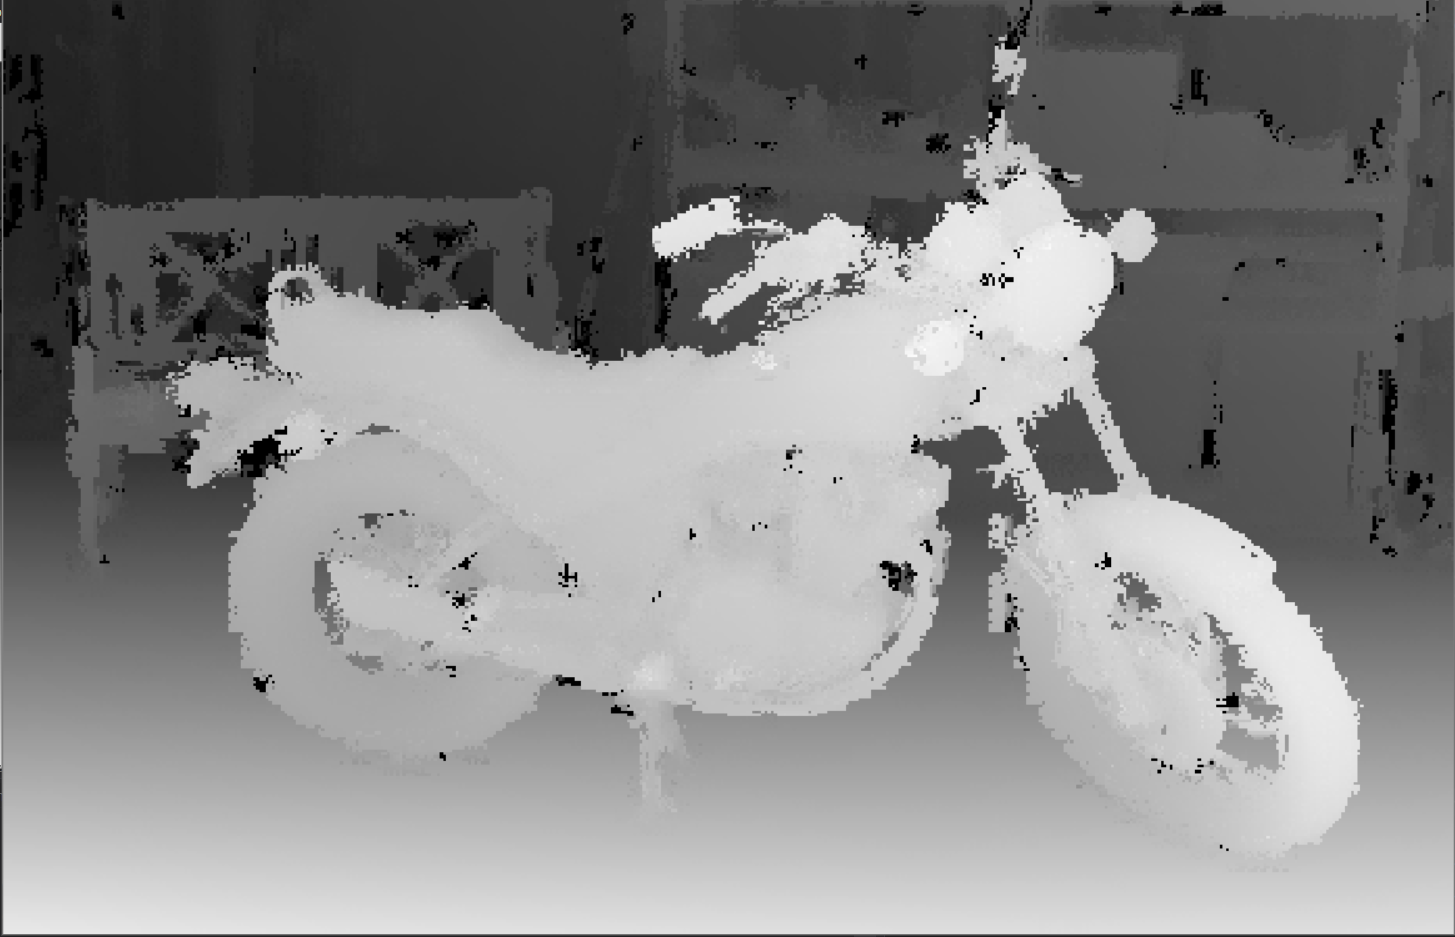
\includegraphics[width=0.4\textwidth, height= 5cm, keepaspectratio]{images/consistency-check-for-deriv-moto.png}
 		\label{fig:consistency-check-moto-01}
}
	\subfigure[No consistency check for derivative calculation]{
 		 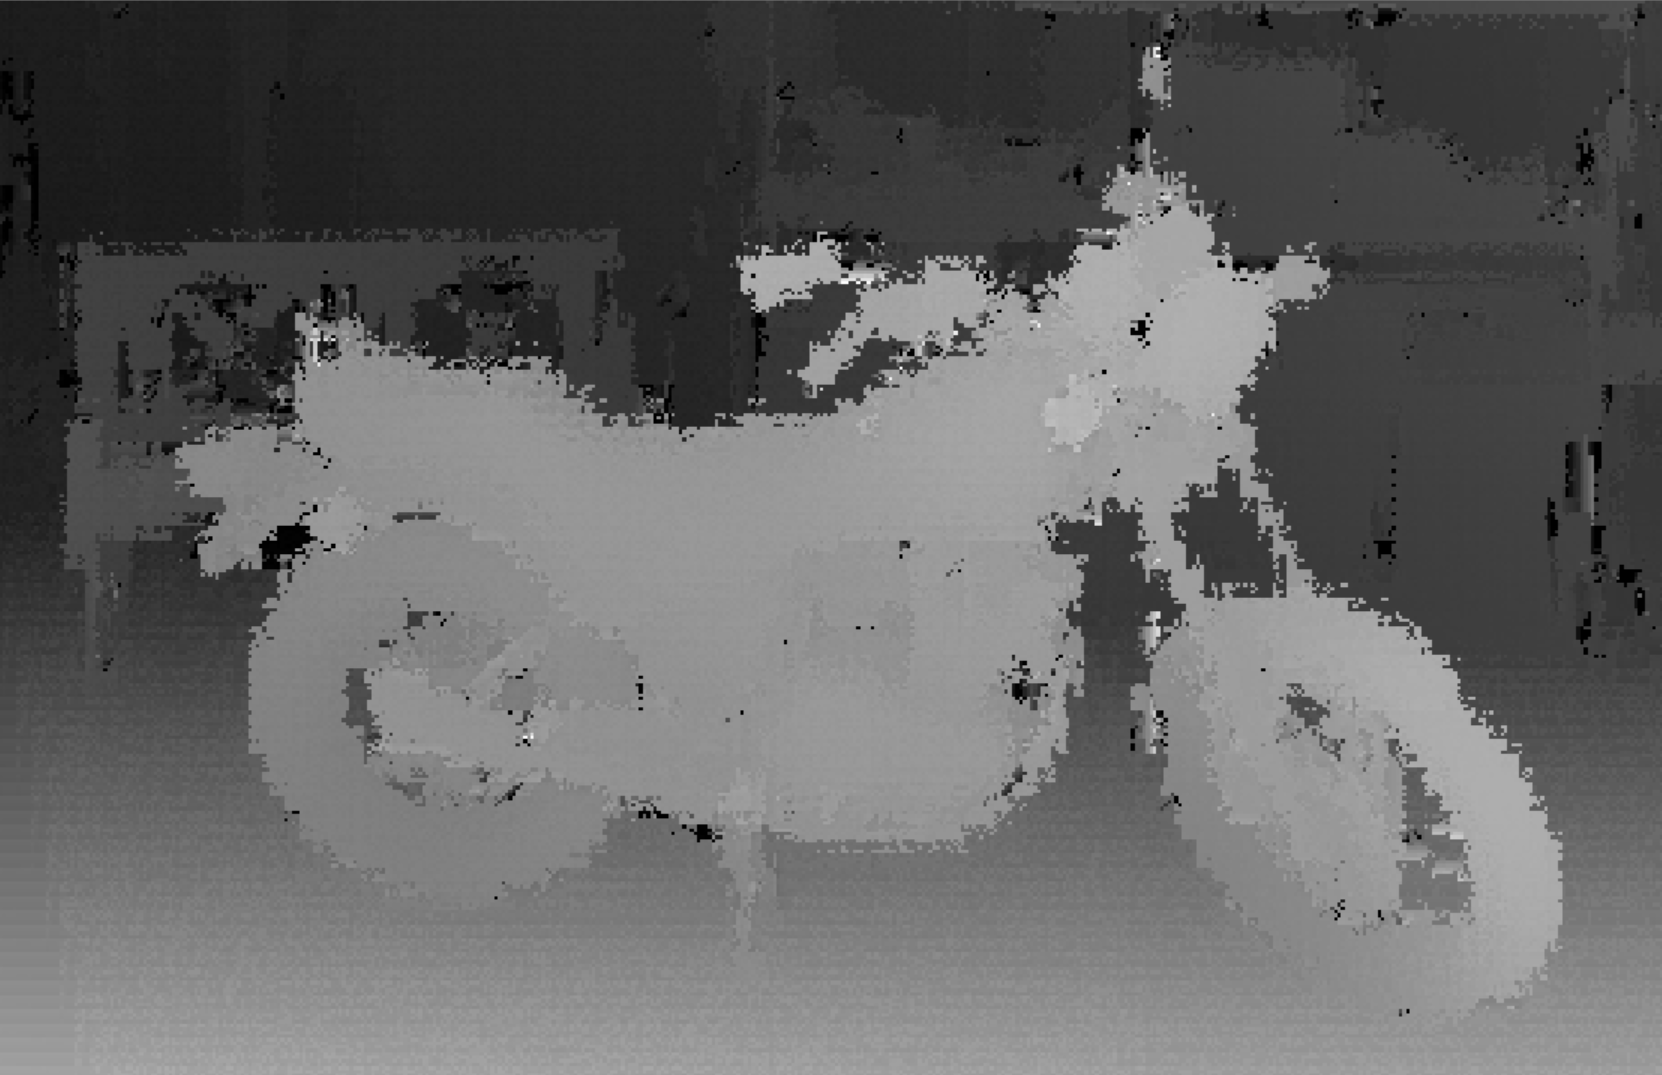
\includegraphics[width=0.4\textwidth, height= 5cm, keepaspectratio]{images/no-consistency-check-for-deriv-moto.png}
 		 \label{fig:no-consistency-check-moto-01}
}
\caption{Comparison between applying and not a consistency check procedure over the same image}
\label{fig:consistency-check-comparison-moto-01}
\end{figure}

During the algorithm designing a specific phase of the pipeline demonstrates to be extremely important. 
Specifically, it consists on the \textit{consistency check} performed during the derivative computation when running the algorithm exploiting the simulated grid of points.
Actually, this consistency check becomes relevant in proximity of the edges, where the magnitude of the $Z$ component of a derivative calculated between two points that belong to far objects, and thus cut by an occlusion, tends to explode.
Therefore, this will affect the estimation procedure, which will most likely carry out wrong values for the computations performed in those areas. \\
Figure~\ref{fig:consistency-check-comparison-moto-01} clearly demonstrate the difference on the final result when the consistency check over the derivatives calculations is applied or not.
When the magnitudes of the derivatives evaluated for a specific points are not correctly adjusted, if a set threshold on the $Z$ components of the derivative vector is exceeded, the final disparity image will show a huge amount of noise, which is obviously related to incorrect estimations.
Figure~\ref{fig:no-consistency-check-moto-01} is the proof of that.
Contrarily, in Figure~\ref{fig:consistency-check-moto-01} a better disparity map is visualized, which comes out when the consistency check operations are carried out.\\
Therefore, since the tests performed over the dataset images and using a simulated point grid, the necessity of the derivative correction was proven to be a valuable, and yet fundamental, step to reach an accurate result.

\subsection{Different thresholds for edge intensity result comparison}
\label{subsection:soft-strong-edge-threshold}

\begin{figure}[t]
	\centering
	\subfigure[Utilization of unique threshold over the whole input grid]{
 		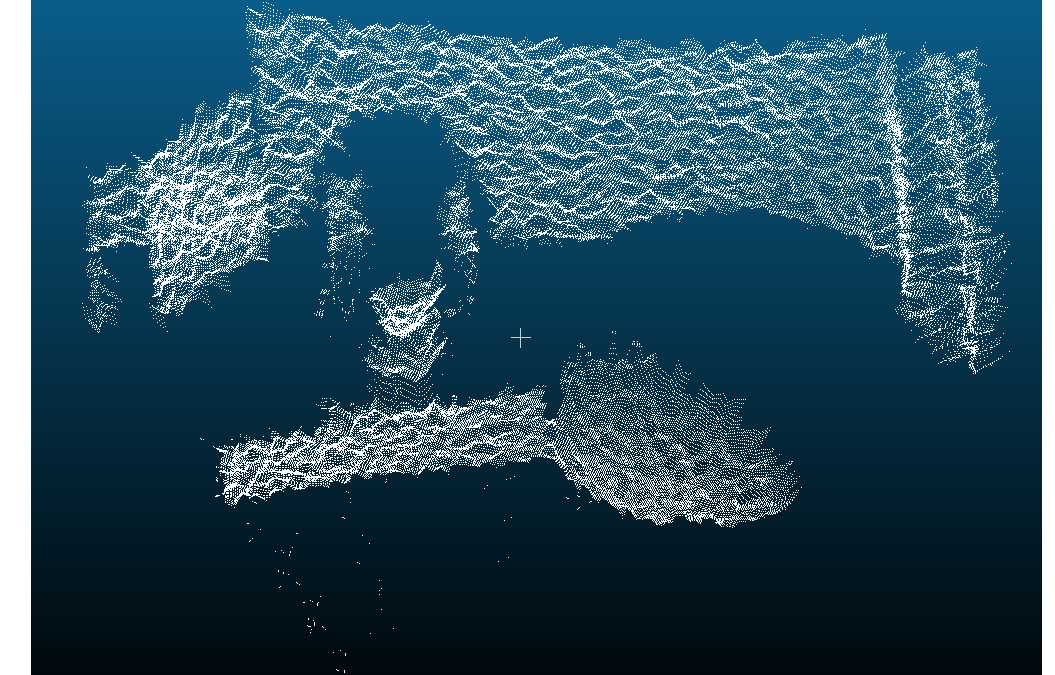
\includegraphics[width=0.4\textwidth, height= 5cm, keepaspectratio]{images/micro-device-result-no-double-threshold-edges.png}
 		\label{fig:single-threshold-micro-01}
}
	\subfigure[Utilization of multiple threshold for distinguish edge strength]{
 		 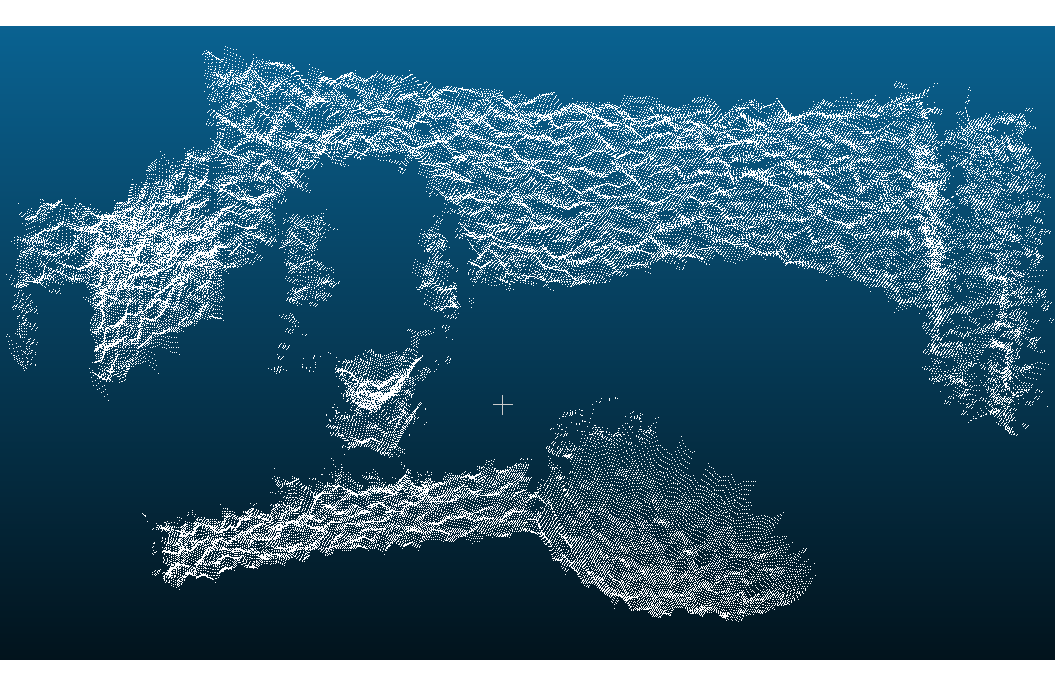
\includegraphics[width=0.4\textwidth, height= 5cm, keepaspectratio]{images/micro-device-result-yes-double-threshold-edges.png}
 		 \label{fig:multiple-threshold-micro-01}
}
\caption{Comparison between utilization of different thresholds distinguish edge strength}
\label{fig:threshold-soft-strong-edges-micro-01}
\end{figure}

Taking into account the results obtained employing the company device, some considerations can be performed in relation to useful improvements that have been implemented to the algorithm during its development. \\
A modification to the initial pipeline of the algorithm, which shows to give interesting improvement in the accuracy of the final 3D point cloud estimated, stands in the utilization of multiple threshold for the edge analysis.
Specifically, as visible in Figure~\ref{fig:single-threshold-micro-01}, utilizing a unique threshold for edge checking over the whole input cloud wrong estimations are generated.
These are depicted in Figure~\ref{fig:single-threshold-micro-01} by the outlier points and are particularly visible where there is not a strong difference in depth among neighbouring point, as it happens between the face of the statue and calibration board on the foreground.\\
On the contrary, when different cases have been implemented in relation to different types of edges, strong and soft, those outliers have gone away, as Figure~\ref{fig:multiple-threshold-micro-01} depicts.


\section{Stereo-matching based method results}
\label{section:stereo-match-results}

Taking into account the results obtained from this method it has to be said that they does not reflect the optimal trade-off compared to the derivative-based algorithm.
As a matter of fact, the computational time of this algorithm is actually relatively long. 
Despite that, the point cloud obtained in output is really dense, as expected, being the algorithm based on pixel-wise computations. 
However, if the results among all the analysed approaches are compared, this increase in density is not worth the rise in computational time, thing that would probably make this method intractable for real time applications.
A real time execution of this approach could be, after all, reached with a proper GPU implementation and setting up a wise construction of the pipeline.
Besides that, its best application could be most likely implied for use cases that need a high level of accuracy by sacrificing proper real time performance.\\
Therefore, the principal comparison could be done between the derivative-based approach, which can be described as a lightweight method, and the standard SGBM method built in OpenCV.


\section{OpenCV method baseline results}
\label{section:opencv-baseline-results}

Comparing the designed lightweight method and the built-in OpenCV SGM-based \texttt{stereoSGBM()} algorithm the following considerations can be provided.\\
First of all, with database images that are taken under optimal conditions and properly adjusted the OpenCV function results to be more accurate and it outputs a more correct disparity map.
The downside is that, it is relatively computationally expensive, at least when executed on a normal laptop exploiting only the CPU.\\
On the other hand, the developed algorithm comes out to be sensibly faster, if run on the same machine and in the same conditions. 
At the same time, it is less accurate, though. 
Regarding that, it has to be underlined that its computation is not optimized.
Moreover, only basic pre and post-processing operations have been applied to its pipeline.
Therefore, it could provide most likely better and more accurate results and probably even in a faster time. \\
Furthermore, an important achievement stands on the use of the initial grid of sparse points.
As a matter of fact, it allows to recover from calibration errors and noise, which are almost unavoidable when images are taken in a real environment under normal conditions.  
Additionally, the input grid helps to deal with texture-less regions of the specific scene, which tend to make the normal SGM method fail. \\
Therefore, at this stage of the work the result obtained with the derivative based method cannot be considered as optimal and the algorithm itself need some further work in order to be considered as competitive in the market, guaranteeing the level of accuracy necessary for providing safety in a real world application.
Nevertheless, the implementation done until this point and the tests accomplished showed that improvements can be provided to reach a high level of accuracy in the estimation, while keeping the computational time in a range suitable for real-time applications. \\
Now, a final overall comparison among the results obtained with all the methods will follow in the next section. 
Some last comments about the achieved outcomes and their suitability are going to be outlined. \\
In conclusion, a final discussion over the overall work is going to be proposed in Chapter~\ref{chapter:discussion}, where considerations about further improvements will be delineated. 
 
\section{Overall comparison of the outcomes}
\label{section:method-comparison}

Summing up the outcomes obtained and the theoretical capabilities of all the different methods studied, the results of the derivative-based method can be considered as accurate result for the purposes of a researching project.
Obviously, when compared over perfect dataset images with properly optimized methods, as the \texttt{stereoSGBM()} available in the OpenCV libraries, a certain lack in accuracy is visible.\\
However, some important features of the designed method, which highlight its potential suitability for real-time computer vision based applications, can be pointed out by analysing the outcomes achieved.
Firstly, a key component of that method is the input grid of sparsified points, which allows to make accurate estimations over all the scene and recover from small calibration errors.
Moreover, that feature supports the possibility of getting accurate results even in texture-less areas of the scene, which are extremely challenging for pure stereo matching based methods.
As a matter of fact, in the literature studied, that was a problem that many researchers tried to overcome in multiple ways, such as designing deep learning based algorithm in the latest years.
In those publications, impressive results have been obtained by improving a standard SGM-based routine with convolutional neural networks.
However, even if they outperforms almost all the previous algorithms, that performance is reached over standard dataset images, such as the Middlebury 2014, KITTI 2012, KITTI 2015 and over synthetic datasets.
Those datasets obviously cover a massive number of real world situations, yet, it would be always possible to deal with environments for which the network has not been properly trained. \\  
Therefore, another core feature of the designed algorithm stands exactly on that.
It can be employed in every kind of scene and it does not need any type of pre-training.
Thus, once it has been embedded in a stereo device, and adjusting the parameters relatively to the hardware specifications, it can provide a dense and accurate 3D point cloud of the scanned scene with a potential real-time performance.

% 
%\chapter{Discussion}
\label{chapter:discussion}

The predetermined main objective of this project was to estimate a 3D dense point cloud starting from an initial sparse set of points and a pair of stereo undistorted images.
Moreover, this overall algorithm should have been executed in real-time, in order to be following embedded in a stereo device, thus to be suitable for autonomous driving, automotive and object detection related purposes.
Therefore, tests for guaranteeing a potentiality for this type of usability have to be carried out. \\
Overall, this can be evaluated as a challenging work, also considering the different algorithms developed since the early nineties in this field, which is considered as one of the most researched areas in computer vision, especially nowadays.\\
Moreover, since the initial stages of the project, there was the need of studying and understanding the company device and, thus, find the optimal way to embed it in the algorithm pipeline.
Additionally a novel strategy has to be thought, making it suitable for the requirements of the uses cases identified and competitive with the current methods.
Furthermore, since the beginning there was the decision to focus on a standard approach, differently from most of the latest algorithms, which are based on deep learning techniques.  
This decision was made in order to do not encounter the problem of the domain shifting, that is the drop in accuracy that most of the CNN-based algorithms face when dealing with new type of environment, especially real ones, on which the network has not been properly trained~\cite{Poggi2019}.
Moreover, another factor that pushed for basing the algorithm on a more standard stereo matching strategy stands on the requirement of being able to embed the algorithm on a relatively small device.
As a matter of fact, one of the company goals is to join the market of single-user devices, designing a product that should be extremely compact.
Therefore, there would be quite infeasible to execute in the stereo system algorithms that requires a high computational cost, such as ones based on neural network structures.
As a matter of fact, in this latter case, pre-training should be developed over an expensive machine, facing again the problem of the environment shifting. \\
Thereby, in order to guarantee a generally accurate result in every possible situation, and for the task of embedding the algorithm on compact devices, the decision was to design a standard based and lightweight method, which would be able to ensure, at least theoretically, a real-time execution.
Considering the whole work done, those tasks were overall achieved.
Surely, further improvements are needed for guaranteeing an extremely fast execution, while keeping a high level of accuracy.
Besides that, if the initial requirements and the different challenges faced during the project development are taken into account, the final result achieved can be considered as a reliable proof of the accomplishment of the initial objective defined.

\section{Overall discussion over the project developed}
\label{section:overall-discussion}

Considering the overall project designed and especially comparing the outcomes achieved with the results of the OpenCV based Semi-Global Block Matching (SGBM) algorithm, which has been used as the baseline, the work done certainly showed that the strategy adopted is actually feasible for the predetermined goals.\\
However, a certain lack in accuracy is visible.
Moreover, the initial pre-processing section of the algorithm should be slightly improved, first of all the calibration of the stereo device, which is still not perfect. \\
Furthermore, more specific post-processing operations should be tested.
As a matter of fact, if multiple pipelines of the algorithm are run in parallel, such as exploiting the left stereo image as the principal one in one case and employing the right one as the primary one in the other case, and implementing at the end a sort of left-right consistency check, a final improved result could be probably achieved. \\
Therefore, defining an overall consideration of the project developed, the main objectives set at the beginning of the work have been generally reached and, as aforementioned, a potential real-time execution of the algorithm has been proved.\\
Hence, successful outcome have been acquired.
Regarding this, the need of further improvements, which would most likely bring the overall project to compete with most of the state-of-the-art methods, can be thought as a valuable target. 

\section{Drawbacks of the designed algorithm}
\label{section:algorithm-drawbacks}

The main advantage of the algorithm developed is that it is sensibly fast.
However, it also hold some side drawbacks, which do not affect its main execution, although they limit the possibility of getting perfect results.\\
As a matter of fact, the algorithm relies a lot on the initial set of points provided through the device, which is surely highly accurate, however it has a certain lack of performance in the detection of small objects.
As specified since the initial chapters, the input points cloud is sparse, thus to ensure the maximum coverage of the scene. 
However, this cannot simultaneously guarantee high performance in terms of accuracy for all the objects in the scene.
Therefore, a more related stereo matching strategy could be employed for those areas, thus to reduce the amount of errors and enhance the overall smoothness and continuity of the final dense cloud.\\
Taking that into account, some approaches have been thought in order to improve the algorithm on that side.
An example would stand on an initial segmentation of the scene.
This will identify the different areas of the analysed environment, and for those regions on which the number of points is below a specific threshold, a more pure SGM based strategy would be applied. 
In fact, the fundamental downside of the classical SGM method is that it is highly expensive, computationally speaking, especially when the disparity range and the image density increase.
Therefore, if the number of disparity levels cannot be reduced drastically, the other feature that can be tackled is the dimension of the analysed area.
Moreover, exploiting the depth information coming from the few points located in the area of interest, the disparity range can be reduced as well.
Hence, if it is applied to small regions, i.e. the segmented areas of small objects, a final potentially real-time execution could be ensured.\\
Another imperfection present in the current version developed is related to the overall smoothness of the estimated 3D cloud.
As a matter of fact, at this stage the estimated point cloud does not present smooth edges and some contours of the objects appears to be a bit rough.
This problem can be effortlessly overcome by running multiple times (most likely two or three times should be enough) the algorithm and using the most accurate points from the previous stage, thus to enhance the density of the final cloud. 
Clearly this hierarchical method will slightly reduce the whole performance, considering that the multiple runs cannot be launched in parallel because the first estimation is needed for the following improvements.
However, in the stages after the first one, not all the computations are produced again, therefore they can be considered as post-processing steps, from a computational point of view, meaning that they will not affect strongly the chance of produce an accurate results in real-time.

\section{Further improvements and future work}
\label{section:further-improvements}

Therefore, some further work will be needed in this project in order to make it reach a level of accuracy that can compete, in terms of accuracy and computational time, with most of the current algorithm designed for depth estimation.
The developed work and the analysis done show a strong potential for the though technique.
Moreover, they prove that the implemented strategy is reasonable for the predetermined scope and the employment of the initial cloud taken from the company device helps in keeping the computation fast and it ensures, at the same time, accurate results.\\
Summing up the development produced, the analysis carried out and the results achieved the following considerations can be outlined.
First of all, the outcomes produced highlight that the strategy thought is reasonable and it allows to obtain generally accurate results in a reasonable time, which could be brought to a real-time performance by implementing the code in the GPU. \\
Secondly, considering the possible further improvements that could be implemented in the code, they mainly concern the smoothness of the final outcome and the point cloud density, which could be highly enhanced by carrying out the algorithm pipeline in a hierarchical manner, exploiting at each stage the increasing number of certainly accurate points. \\
Moreover, the idea of including some segmentation on the input rectified images, in the pre-processing stage, in order to identify the regions that contain a low amount of initial point, would be analysed.
The main scope of that would be improving the densification, i.e. the object reconstruction, in those areas where the laser points are limited, so that the estimation errors could easily decrease. 
Additionally, in the real environment images taken with the company device, areas with clusters of missing date have been observed close to edges, i.e. occluded regions. 
In the current implementation a initial pre-estimation of the 3D position of those points is realized by exploiting the data from the neighboring points. \\
However, in some region, because of the relatively high amount of missing data, an accurate generation of data was not possible, therefore, in those cases, it has been preferred to discard those points, thus to not affect the following estimations with wrong initial data.
Anyway, the amount of those missing data do not influence strongly the whole procedure, considering that those points are only among 2.5 and the 5\% with respect to the entire initial cloud. 
Therefore, that amount of initial can be accepted, being a reasonable percentage when dealing with real world data. 

% 
%\chapter{Conclusions}
\label{chapter:conclusions}

Time to wrap it up!  Write down the most important findings from your
work.  Like the introduction, this chapter is not very long.  One to
two (never over three) pages might be a good limit. Still, the chapter
gives the background, goals, content, and the findings. However, all that
should already be in the previous chapters. This is just a summary (as
are the abstract and the introduction).

For making PDF/A version requested by the Aalto Library, open the end result pdf file in Acrobat and store it as PDF/A. Then verify the result (everything should be fine, at least as PDF/A-2b version works).

Congratulations, your thesis is ready and it looks beautiful!



% Load the bibliographic references
% ------------------------------------------------------------------
% You can use several .bib files:
% \bibliography{thesis_sources,ietf_sources}
\bibliography{sources}


% Appendices go here
% ------------------------------------------------------------------
% If you do not have appendices, comment out the following lines
\appendix
\chapter{First appendix}
\label{chapter:first-appendix}

This is the first appendix. You could put some test images or verbose data in an
appendix, if there is too much data to fit in the actual text nicely.

For now, the Aalto logo variants are shown in Figure~\ref{fig:aaltologo}.

\begin{figure}
\begin{center}
\subfigure[In English]{
\includegraphics[width=.8\textwidth]{images/aalto-logo-en}}
\caption{Aalto logo variants}
\label{fig:aaltologo}
\end{center}
\end{figure}


% End of document!
% ------------------------------------------------------------------
% The LastPage package automatically places a label on the last page.
% That works better than placing a label here manually, because the
% label might not go to the actual last page, if LaTeX needs to place
% floats (that is, figures, tables, and such) to the end of the 
% document.
\end{document}
















